% Options for packages loaded elsewhere
\PassOptionsToPackage{unicode}{hyperref}
\PassOptionsToPackage{hyphens}{url}
%
\documentclass[
]{book}
\usepackage{amsmath,amssymb}
\usepackage{lmodern}
\usepackage{ifxetex,ifluatex}
\ifnum 0\ifxetex 1\fi\ifluatex 1\fi=0 % if pdftex
  \usepackage[T1]{fontenc}
  \usepackage[utf8]{inputenc}
  \usepackage{textcomp} % provide euro and other symbols
\else % if luatex or xetex
  \usepackage{unicode-math}
  \defaultfontfeatures{Scale=MatchLowercase}
  \defaultfontfeatures[\rmfamily]{Ligatures=TeX,Scale=1}
\fi
% Use upquote if available, for straight quotes in verbatim environments
\IfFileExists{upquote.sty}{\usepackage{upquote}}{}
\IfFileExists{microtype.sty}{% use microtype if available
  \usepackage[]{microtype}
  \UseMicrotypeSet[protrusion]{basicmath} % disable protrusion for tt fonts
}{}
\makeatletter
\@ifundefined{KOMAClassName}{% if non-KOMA class
  \IfFileExists{parskip.sty}{%
    \usepackage{parskip}
  }{% else
    \setlength{\parindent}{0pt}
    \setlength{\parskip}{6pt plus 2pt minus 1pt}}
}{% if KOMA class
  \KOMAoptions{parskip=half}}
\makeatother
\usepackage{xcolor}
\IfFileExists{xurl.sty}{\usepackage{xurl}}{} % add URL line breaks if available
\IfFileExists{bookmark.sty}{\usepackage{bookmark}}{\usepackage{hyperref}}
\hypersetup{
  pdftitle={An Introduction to Experimental Design and Linear Models},
  pdfauthor={Andrew P Beckerman (based on text and slides from Mark Rees and Gareth Phoenix)},
  hidelinks,
  pdfcreator={LaTeX via pandoc}}
\urlstyle{same} % disable monospaced font for URLs
\usepackage{color}
\usepackage{fancyvrb}
\newcommand{\VerbBar}{|}
\newcommand{\VERB}{\Verb[commandchars=\\\{\}]}
\DefineVerbatimEnvironment{Highlighting}{Verbatim}{commandchars=\\\{\}}
% Add ',fontsize=\small' for more characters per line
\usepackage{framed}
\definecolor{shadecolor}{RGB}{248,248,248}
\newenvironment{Shaded}{\begin{snugshade}}{\end{snugshade}}
\newcommand{\AlertTok}[1]{\textcolor[rgb]{0.94,0.16,0.16}{#1}}
\newcommand{\AnnotationTok}[1]{\textcolor[rgb]{0.56,0.35,0.01}{\textbf{\textit{#1}}}}
\newcommand{\AttributeTok}[1]{\textcolor[rgb]{0.77,0.63,0.00}{#1}}
\newcommand{\BaseNTok}[1]{\textcolor[rgb]{0.00,0.00,0.81}{#1}}
\newcommand{\BuiltInTok}[1]{#1}
\newcommand{\CharTok}[1]{\textcolor[rgb]{0.31,0.60,0.02}{#1}}
\newcommand{\CommentTok}[1]{\textcolor[rgb]{0.56,0.35,0.01}{\textit{#1}}}
\newcommand{\CommentVarTok}[1]{\textcolor[rgb]{0.56,0.35,0.01}{\textbf{\textit{#1}}}}
\newcommand{\ConstantTok}[1]{\textcolor[rgb]{0.00,0.00,0.00}{#1}}
\newcommand{\ControlFlowTok}[1]{\textcolor[rgb]{0.13,0.29,0.53}{\textbf{#1}}}
\newcommand{\DataTypeTok}[1]{\textcolor[rgb]{0.13,0.29,0.53}{#1}}
\newcommand{\DecValTok}[1]{\textcolor[rgb]{0.00,0.00,0.81}{#1}}
\newcommand{\DocumentationTok}[1]{\textcolor[rgb]{0.56,0.35,0.01}{\textbf{\textit{#1}}}}
\newcommand{\ErrorTok}[1]{\textcolor[rgb]{0.64,0.00,0.00}{\textbf{#1}}}
\newcommand{\ExtensionTok}[1]{#1}
\newcommand{\FloatTok}[1]{\textcolor[rgb]{0.00,0.00,0.81}{#1}}
\newcommand{\FunctionTok}[1]{\textcolor[rgb]{0.00,0.00,0.00}{#1}}
\newcommand{\ImportTok}[1]{#1}
\newcommand{\InformationTok}[1]{\textcolor[rgb]{0.56,0.35,0.01}{\textbf{\textit{#1}}}}
\newcommand{\KeywordTok}[1]{\textcolor[rgb]{0.13,0.29,0.53}{\textbf{#1}}}
\newcommand{\NormalTok}[1]{#1}
\newcommand{\OperatorTok}[1]{\textcolor[rgb]{0.81,0.36,0.00}{\textbf{#1}}}
\newcommand{\OtherTok}[1]{\textcolor[rgb]{0.56,0.35,0.01}{#1}}
\newcommand{\PreprocessorTok}[1]{\textcolor[rgb]{0.56,0.35,0.01}{\textit{#1}}}
\newcommand{\RegionMarkerTok}[1]{#1}
\newcommand{\SpecialCharTok}[1]{\textcolor[rgb]{0.00,0.00,0.00}{#1}}
\newcommand{\SpecialStringTok}[1]{\textcolor[rgb]{0.31,0.60,0.02}{#1}}
\newcommand{\StringTok}[1]{\textcolor[rgb]{0.31,0.60,0.02}{#1}}
\newcommand{\VariableTok}[1]{\textcolor[rgb]{0.00,0.00,0.00}{#1}}
\newcommand{\VerbatimStringTok}[1]{\textcolor[rgb]{0.31,0.60,0.02}{#1}}
\newcommand{\WarningTok}[1]{\textcolor[rgb]{0.56,0.35,0.01}{\textbf{\textit{#1}}}}
\usepackage{longtable,booktabs,array}
\usepackage{calc} % for calculating minipage widths
% Correct order of tables after \paragraph or \subparagraph
\usepackage{etoolbox}
\makeatletter
\patchcmd\longtable{\par}{\if@noskipsec\mbox{}\fi\par}{}{}
\makeatother
% Allow footnotes in longtable head/foot
\IfFileExists{footnotehyper.sty}{\usepackage{footnotehyper}}{\usepackage{footnote}}
\makesavenoteenv{longtable}
\usepackage{graphicx}
\makeatletter
\def\maxwidth{\ifdim\Gin@nat@width>\linewidth\linewidth\else\Gin@nat@width\fi}
\def\maxheight{\ifdim\Gin@nat@height>\textheight\textheight\else\Gin@nat@height\fi}
\makeatother
% Scale images if necessary, so that they will not overflow the page
% margins by default, and it is still possible to overwrite the defaults
% using explicit options in \includegraphics[width, height, ...]{}
\setkeys{Gin}{width=\maxwidth,height=\maxheight,keepaspectratio}
% Set default figure placement to htbp
\makeatletter
\def\fps@figure{htbp}
\makeatother
\setlength{\emergencystretch}{3em} % prevent overfull lines
\providecommand{\tightlist}{%
  \setlength{\itemsep}{0pt}\setlength{\parskip}{0pt}}
\setcounter{secnumdepth}{5}
\usepackage{booktabs}
\usepackage{amsthm}
\makeatletter
\def\thm@space@setup{%
  \thm@preskip=8pt plus 2pt minus 4pt
  \thm@postskip=\thm@preskip
}
\makeatother
\ifluatex
  \usepackage{selnolig}  % disable illegal ligatures
\fi
\usepackage[]{natbib}
\bibliographystyle{apalike}

\title{An Introduction to Experimental Design and Linear Models}
\author{Andrew P Beckerman (based on text and slides from Mark Rees and Gareth Phoenix)}
\date{2021-02-09}

\begin{document}
\maketitle

{
\setcounter{tocdepth}{1}
\tableofcontents
}
\hypertarget{introduction}{%
\chapter{Introduction}\label{introduction}}

Welcome to An Introduction to Experimental Design and Linear Models

In this mini-module, you'll be learning about the design and analysis of ANOVA and ANCOVA experiments.

This module is compulsory for all, because it forms the foundation for most of the more complex experiments you will do as a researcher. And it is the major step beyond the t-test, 1-way ANOVA, simple regression and chi-square contingency table analyses we covered in semester 1.

If you found Semester 1 ideas hard, please return to the sections on the 1-way ANOVA and the Regression model. Chapter 5 in Getting Started with R (available as an online Resource via STARPlus) covers the material you should know.

You will also need to feel comfortable with dplyr and ggplot - well be reinforcing the old stuff and introducing a few new tricks.

There are 12 Chapters to the book, some only a page or two and some quite a but longer. The majority contain R code that you should recreated in your own scripts as you work along. You should use your scripts to add annotation and notes about the core ideas.

The learning outcome for this mini-module are that you will understand the basic ideas about

\begin{itemize}
\tightlist
\item
  Replication, Randomisation and Reducing Noise
\item
  Experimental Design and Analysis - The Completely Randomised Design
\item
  Experimental Design and Analysis - The Randomised Block Design
\item
  Experimental Design and Analysis - The Latin Square Design
\item
  Experimental Design and Analysis - The ANCOVA Design
\item
  Multiple Regression and Non-linearity.
\end{itemize}

A note on time allocation: In a `normal semester', you'd be in the computer room working on these topics for \textasciitilde12 hours over the course of 3 days in a week.

You should plan on allocating 9-12 hours of your week to this section. You should expect to do the same for the other mini-modules.

\hypertarget{the-three-rs}{%
\subsection{The Three Rs}\label{the-three-rs}}

Before we get started, it's vital that you understand that there are some very basic principles needed to ensure that your experiments can provide robust and reliable inference (answers to your questions). The ``3 R's''.

\begin{itemize}
\tightlist
\item
  \textbf{Randomisation}: the random allocation of treatments to the experimental units, to avoid confounding between treatment effects and other unknown effects.
\item
  \textbf{Replication}: the repetition of a treatment within an experiment, to quantify the natural variation between experimental units and increase accuracy of estimated effects.
\item
  \textbf{Reduce noise:} by controlling as much as possible the conditions in the experiment, e.g.~by grouping of similar experimental units in blocks.
\end{itemize}

As we develop ideas, you should come back to these definitions and see if your understanding of them has improved.

\hypertarget{the-general-linear-model}{%
\subsection{The General Linear Model}\label{the-general-linear-model}}

This module is focused on a class of model called the General Linear Model. It is not a \textbf{GLM}. The \textbf{GLM} is a generalised linear model. I know, right?

The general linear model is, as we learned last semester, a model fit in R with the \texttt{lm()} function. It includes regression, ANOVA, ANCOVA and variations of these. There are a few key characterstics to remember about these models

The general linear model has the following form

\(y = \beta_{0}+\beta_{1}*X_{1}+\beta_{2}*X_{2}+\epsilon\)

Where the \(y\) is the response variable, the \(\beta\)'s are estimated parameters, the \(X\)'s are the predictor variables and the \(\epsilon\) comes from a Gaussian distribution with zero mean and constant variance.

Let's decompose that a bit more

There are two types of predictor variable

Metric predictor variables are measurements of some quantity that may help to predict the value of the response. For example, if the response is the blood pressure of patients in a clinical trial, then age, fat mass and height are potential metric predictor variables. You may know these as \textbf{continuous explanatory variables}

Factor variables are labels that serve to categorize the response measurements into groups, which may have different expected values. Continuing the blood pressure example, factor variables might be sex and drug treatment received (drug A, drug B or placebo, for example). You may also know these as \textbf{categorical explanatory variables}.

So, you hopefully can see how this \emph{general} linear model is capable of representing

\begin{enumerate}
\def\labelenumi{\arabic{enumi}.}
\tightlist
\item
  ANOVA -- Analysis of variance. Predictors are factors.
\item
  Regression. Predictor is a metric variable (continuous variable).\\
\item
  Multiple regression. Predictors are a metric variables (continuous variables).
\item
  ANCOVA - Analysis of co-variance. Predictors are a mixture of metric variables (continuous variables) and factors.
\end{enumerate}

Finally, it is important to understand that these data can be modelled with a linear model:

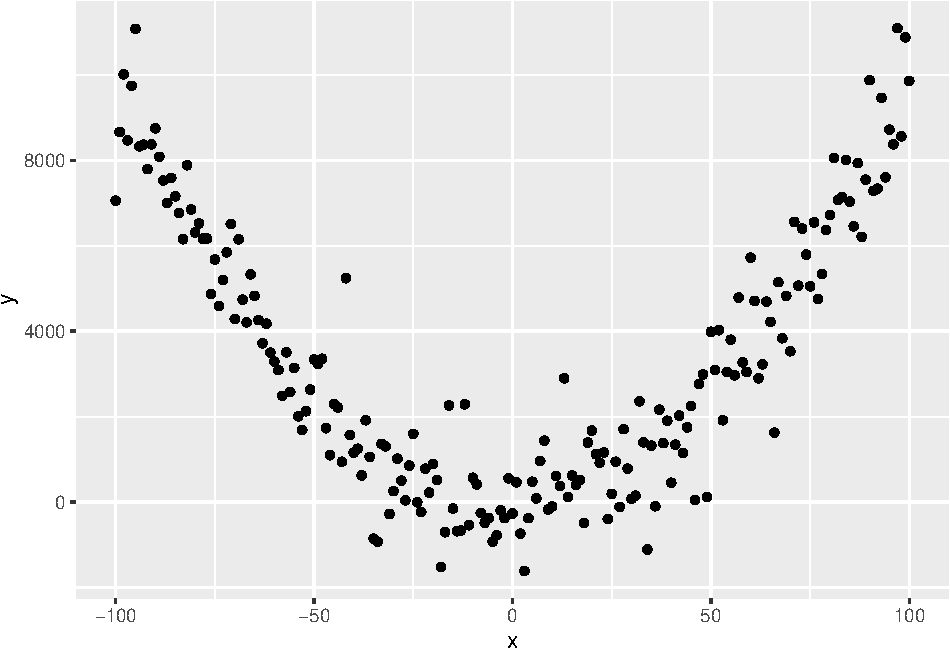
\includegraphics{Introduction-to-Experimental-Design-and-Analysis_files/figure-latex/unnamed-chunk-2-1.pdf}

How, you ask!? Well\ldots. consider this equation

\(y = 0.01 + x + x^{2} + \epsilon\)

Referring to our generic model structure above,

\(y = \beta_{0}+\beta_{1}*X_{1}+\beta_{2}*X_{2}+\epsilon\)

we hopefully can see that \(\beta_{0} = 0.01\), \(\beta_{1} = 0\) and \(\beta_{2} = 1\), where \(X_{2} = X^{2}\)!

Linear models are perfectly capable of being used to estimate non-linear relationships.

Here is the code to make that figure.

\begin{Shaded}
\begin{Highlighting}[]
\CommentTok{\# set x range}
\NormalTok{x }\OtherTok{\textless{}{-}} \SpecialCharTok{{-}}\DecValTok{100}\SpecialCharTok{:}\DecValTok{100}
\CommentTok{\# define y without error}
\NormalTok{y\_det }\OtherTok{\textless{}{-}} \FloatTok{0.01}\SpecialCharTok{+}\NormalTok{x}\SpecialCharTok{\^{}}\DecValTok{2}
\CommentTok{\# add some random variation}
\NormalTok{y }\OtherTok{\textless{}{-}}\NormalTok{ y\_det}\SpecialCharTok{+}\FunctionTok{rnorm}\NormalTok{(}\FunctionTok{length}\NormalTok{(x),}\DecValTok{0}\NormalTok{,}\DecValTok{1000}\NormalTok{)}

\CommentTok{\# create dataframe and plot}
\NormalTok{df }\OtherTok{\textless{}{-}} \FunctionTok{data.frame}\NormalTok{(x, y)}
\FunctionTok{ggplot}\NormalTok{(df, }\FunctionTok{aes}\NormalTok{(}\AttributeTok{x =}\NormalTok{ x, }\AttributeTok{y =}\NormalTok{ y))}\SpecialCharTok{+}
  \FunctionTok{geom\_point}\NormalTok{()}
\end{Highlighting}
\end{Shaded}

\hypertarget{section-readings--}{%
\subsection{Section Readings ----}\label{section-readings--}}

There are several resources that will help with this section of the stats course, and onwards

\begin{itemize}
\tightlist
\item
  Getting Started with R - An Introducton for Biologists, Second Edition (available as an electronic online resource via StarPlus)
\item
  Experimental Design for the Life Sciences - Nick Colegrave and Graham Ruxton (seen on eBay for £2.50!)
\item
  Of course, the venerable coursebook for APS 240: \url{https://dzchilds.github.io/stats-for-bio/index.html}
\end{itemize}

\hypertarget{install-some-extra-packages--}{%
\subsection{Install some extra packages ----}\label{install-some-extra-packages--}}

In order to make this module more effective, we are going to use some additional resources from CRAN.

Please install these packages, if you have not already, using the install packages tab in RStudio:

\begin{itemize}
\tightlist
\item
  \texttt{tidyverse}
\item
  \texttt{ggfortify}
\item
  \texttt{agricolae}
\item
  \texttt{car}
\item
  \texttt{gmodels}
\item
  \texttt{visreg}
\item
  \texttt{patchwork}
\end{itemize}

\hypertarget{intro}{%
\chapter{Introduction To Experiments (Some Philosophy)}\label{intro}}

Experiments help us answer questions, but there are also non-experimental techniques. What is so special about experiments?

\begin{enumerate}
\def\labelenumi{\arabic{enumi}.}
\tightlist
\item
  Experiments allow us to set up a direct comparison between the treatments of interest.
\item
  We can design experiments to minimize any bias in the comparison.
\item
  We can design experiments so that the error in the comparison is small.
\item
  Most important, we are in control of experiments, and having that control
  allows us to make stronger inferences about the nature of differences
  that we see in the experiment. Specifically, we may make inferences
  about causation.
\end{enumerate}

This last point distinguishes an experiment from an observational study. In an observational study we merely observe which units are in which treatment groups; we don't get to control that assignment. This underpins the classic issue with assigning \emph{causation to correlation} - in the following two examples, there is a strong association between the variables, but there has been no control/manipulation.

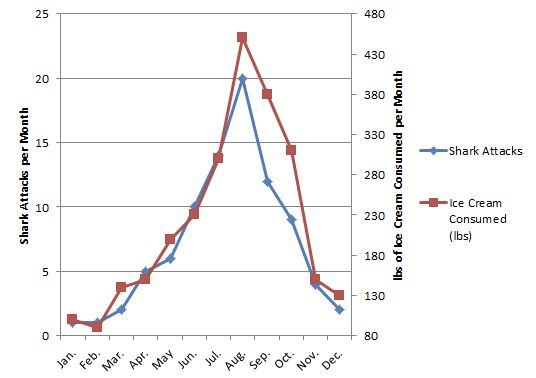
\includegraphics[width=7.44in]{images/IceCream_Shark}
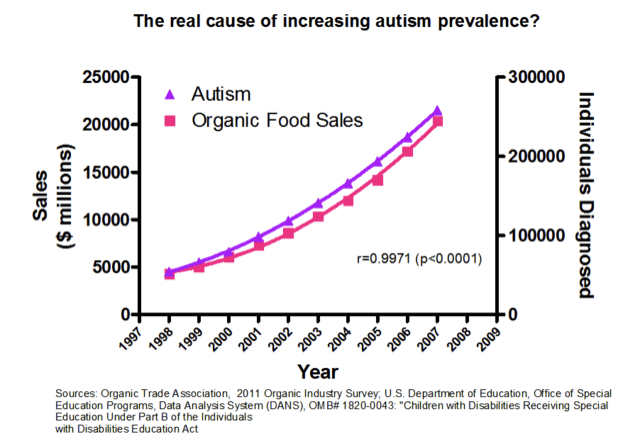
\includegraphics[width=8.89in]{images/Autism_Organic}

Mosteller and Tukey (1977) list three concepts associated with causation and state that two or three are needed to support a causal relationship:

\begin{itemize}
\tightlist
\item
  Consistency -- make a change and the response is in the same direction or the amount of response is \emph{consistent} across populations
\item
  Responsiveness -- make a change and the response changes according to theory
\item
  Mechanism -- make a change and we can monitor/identify a mechanism leading from cause to effect
\end{itemize}

Let's look at a classic example. Smoking and lung cancer -- from 1922 to 1947 annual deaths for lung cancer went from 612 to 9287 (Observation).This was thought in the 1950s to be either an effect of smoking tobacco or atmospheric pollution (Hypothesis). Numerous studies showed that lung cancer was more prevalent in smokers (Observation: consistency). Chemical analyses of tobacco showed it contained carcinogens (Association: mechanism). Public health programs resulted in a reduction in smoking and lung cancer rates decreased (Intervention: responsiveness).

Note the initial study was an observational study and in this case it was not ethical to do the experiment per se!

\hypertarget{how-to-think-about-experiments-components-of-an-experiment}{%
\section{How to think about experiments: Components of an Experiment}\label{how-to-think-about-experiments-components-of-an-experiment}}

An experiment has treatments, experimental units, responses, and a method to assign treatments to units. These specify the experimental design.

Not all experimental designs are created equal. A good experimental design must adhere to the 3Rs. It should reveal consistency, responsiveness and mechanism. The way this happens is by avoiding systematic error in measuring things, and allow estimation of error in measurments with precision. In short, a good experimental design must

\begin{itemize}
\tightlist
\item
  Avoid systematic error
\item
  Allow estimation of error
\item
  Be precise
\item
  Have broad validity.
\end{itemize}

Lets walk through some definitions.

If our experiment has \emph{systematic error}, then our comparisons will be biased, no matter how precise our measurements are or how many experimental units we use. \textbf{Randomisation} is our tool to combat \emph{systematic error}.

Even without \emph{systematic error}, there will be random error in the responses - this is what we call variation in what we are measuring or more formally variance. Such variation in responses invariably leads to random error in the treatment comparisons. When we compared two means in the t-test, we had to deal with the variation in both groups!

Experiments are precise when this random error in the treatment comparisons is small. Precision depends on the size of the random errors in the responses, the number of units used (\textbf{replication}), and the experimental design used.

Experiments must be designed so that we have an estimate of the size of random error. This permits statistical inference: for example, confidence intervals or tests of significance based on t- or F-statistics.

We cannot do inference without an estimate of this variation. We would like our conclusions to be valid for a wide population, so we need to randomise our subjects or objects we are measuring - for example, we may need to be aware of both sexes and of young and old individuals. But there are always compromises - for example, broadening the scope of validity by using a variety of experimental units may decrease the precision of the responses.

\hypertarget{how-do-we-increase-precision-and-reduce-bias}{%
\subsection{How do we increase precision and reduce bias?}\label{how-do-we-increase-precision-and-reduce-bias}}

There are several key concepts

\hypertarget{blinding}{%
\subsubsection{Blinding}\label{blinding}}

\emph{Blinding} occurs when the evaluators of a response do not know which treatment was given to which unit. Blinding helps prevent bias in the evaluation, even unconscious bias from well-intentioned evaluators. Double blinding occurs when both the evaluators of the response and the (human subject) experimental units do not know the assignment of treatments to units. Blinding the subjects can also prevent bias, because subject responses can change when subjects have expectations for certain treatments.

\hypertarget{placebos}{%
\subsubsection{Placebos}\label{placebos}}

\emph{Placebo} is a null treatment that is used when the \emph{act} of applying a treatment--- any treatment --- has an effect. Placebos are often used with human subjects, because people often respond to the process of receiving any treatment: for example,
reduction in headache pain when given a sugar pill. Blinding is important when placebos are used with human subjects. Placebos are also useful for nonhuman subjects. The apparatus for spraying a field with a pesticide may compact the soil. Thus we drive the apparatus over the field, without actually spraying, as a placebo treatment.

\hypertarget{confounders}{%
\subsubsection{Confounders}\label{confounders}}

\emph{Confounding} occurs when the effect of one factor or treatment cannot be distinguished from that of another factor or treatment. The two factors or treatments are said to be confounded. Except in very special circumstances, confounding should be avoided. Consider the following example. We plant corn variety A in Yorkshire and corn variety B in Lancashire. In this experiment, we cannot distinguish location effects (Yorkshire vs.~Lancashire) from variety effects (cornA vs.~cornB) --- the variety factor and the location factor are confounded.

This is despite the fact that we know that Yorkshire will be better\ldots. (that's a joke)

\hypertarget{experimental-vs-measurement-units}{%
\section{Experimental vs Measurement units}\label{experimental-vs-measurement-units}}

A common source of difficulty in designing experiments is the distinction between experimental units and measurement units. We need to know the experimental units, as this is the key value used to generate our inference.

Consider an educational study, with six classrooms of 25 pupils. Each classroom of students is then assigned, at random, to one of two different reading programmes.

At the end of a 6 week term, all the students are evaluated via a common reading exam.

So, are there six experimental units (the classrooms) or 150 (25*6; the students)? We measured the reading ability of the students\ldots{} but they were in classroom sets of 25\ldots.

\hypertarget{identifying-the-experimental-unit---an-example-of-pseudo-replication}{%
\subsubsection{\texorpdfstring{Identifying the experimental unit - an example of \textbf{pseudo-replication}}{Identifying the experimental unit - an example of pseudo-replication}}\label{identifying-the-experimental-unit---an-example-of-pseudo-replication}}

To identify the experimental units the key question is: What did we randomly allocate treatments to?

If we randomly allocated reading programmes to students, then students would be the experimental units. But we don't so the classroom is the experimental unit -- it is the classroom to which we randomly allocated treatments. The classroom is the experimental unit. But we don't measure how a classroom reads; we measure how students read. Thus students are the measurement units for this experiment.

Confusing these two things can lead to \textbf{pseudo-replication}. Treating measurement units as experimental usually leads to overoptimistic analysis --- we will reject null hypotheses more often than we should, and our confidence intervals will be too narrow. The usual way around this is to determine a single response for each experimental unit.

\hypertarget{this-really-matters.}{%
\subsubsection{This really matters.}\label{this-really-matters.}}

Consider an experiment with 2 growth chambers each containing 100 plants. One of the chambers received enhanced C02. One night after collecting data you leave the door open on the C02 chamber and the temperature drops and so the plants grow more slowly. When you come to analyze the data you get a highly significant effect but C02 results in reduced plant growth not what you expect.

This is entirely plausible.

Consider a second experiment where you really do have 200 growth chambers and randomly allocate plants to each. If you forget to close one door it really has no effect as just one plant is affected.

To get the same effect as in the first experiment you would have to accidentally leave the doors open on all the C02 chambers. This is very unlikely indeed!!!

There are 9x1058 ways selecting 100 chambers from 200 chambers so the chance of accidentally picking all the C02 chambers is 1/ 9x10580 (stars in universe 7 x 1022).

Proper \textbf{randomization} and \textbf{replication} is very different from \textbf{pseudo-replication}.

\hypertarget{take-home-message-randomization-properly-with-replication-protects-against-confounding}{%
\subsection{Take Home Message: Randomization properly with Replication protects against Confounding}\label{take-home-message-randomization-properly-with-replication-protects-against-confounding}}

\begin{quote}
An experiment is randomized if the method for assigning treatments to units involves a known, well-understood probabilistic scheme. The probabilistic scheme is called a randomization.
\end{quote}

\begin{quote}
In general, more experimental units with fewer measurement units per experimental unit works better. However, smaller experimental units are inclined to have greater edge effect problems than are larger units, so this recommendation needs to be moderated by consideration of the actual units.
\end{quote}

No matter which features of the population of experimental units are associated with our response, our randomizations put approximately \emph{half the individuals with these features} into \emph{each treatment group}.

Recall our example above of considering sex and age of subjects and imagine a treatment with two levels (hot and cold). Done well, proper randomisation will put approximately half the males, half the females, half the older, half the youger etc into each of the treatment levels.

The beauty of randomization is that it helps prevent confounding, even for factors that we do not know are important.

\hypertarget{a-non-randomized-experiment-haphazard-is-not-randomized}{%
\subsection{\texorpdfstring{A non-randomized experiment -- \textbf{haphazard} is NOT randomized}{A non-randomized experiment -- haphazard is NOT randomized}}\label{a-non-randomized-experiment-haphazard-is-not-randomized}}

A company is evaluating two different word processing packages for use by its clerical staff. Part of the evaluation is how quickly a test document can be entered correctly using the two programs. We have 20 test secretaries, and each secretary will enter the document twice, using each program once.

Suppose that all secretaries did the evaluation in the order A first and B second. Does the second program have an advantage because the secretary will be familiar with the document and thus enter it faster? Or maybe the second program will be at a disadvantage because the secretary will be tired and thus slower.

Randomization generally costs little in time and trouble, but it can save us from \texttt{disaster}.

Anything that might affect your responses should be randomized! For example

\begin{itemize}
\tightlist
\item
  If the experimental units are not used simultaneously, you can randomize the order in which they are used.
\item
  If the experimental units are not used at the same location, you can randomize the locations at which they are used.
\item
  If you use more than one measuring instrument for determining response, you can randomize which units are measured on which instruments.
\end{itemize}

\hypertarget{mini-quiz}{%
\section{Mini-Quiz}\label{mini-quiz}}

\begin{quote}
A PhD student want to determine the effects of protein on beetle fecundity so they design an experiment with a control and protein enhanced diet. To assign beetles to each of the treatments they pour a culture onto the table and catch the first 30 beetles that run to the edge of the table, these receive the protein enhanced diet. The next 30 beetles go in the control. \textbf{Is this randomized?}
\end{quote}

\hypertarget{replication-how-many}{%
\section{Replication: How many?}\label{replication-how-many}}

No simple rules\ldots{} it depends\ldots{} on\ldots.

\begin{itemize}
\tightlist
\item
  Resources available
\item
  Variability of experimental units
\item
  Treatment structure -- more later
\item
  Size of effect that's important
\item
  Relative importance of different comparisons
\end{itemize}

There is, however, a set of tools that can help with estimating sample sizes. It's called power analysis and requires that you have some a priori estimate of the expected variation in your response variable.

\hypertarget{standard-errors-precision-and-sampling}{%
\chapter{Standard Errors, Precision and Sampling}\label{standard-errors-precision-and-sampling}}

\hypertarget{standard-errors-and-precision}{%
\section{Standard Errors and precision}\label{standard-errors-and-precision}}

One of the most important statistical metrics to wrap your heads around is the standard error of the mean.

We introduced this in the first semester and there is a good discussion of it in the APS 240 reading. You should re-read this section:

\url{https://dzchilds.github.io/stats-for-bio/sampling-error.html}

The take home message is that the standard error is a quantitative measure of sampling error variation. It is also very sensitive to the sample size, because the equation is \texttt{sd(variable)/sqrt(sample\_size)}. As the sample size increases, the standard error, an estimate of the sampling error, goes down.

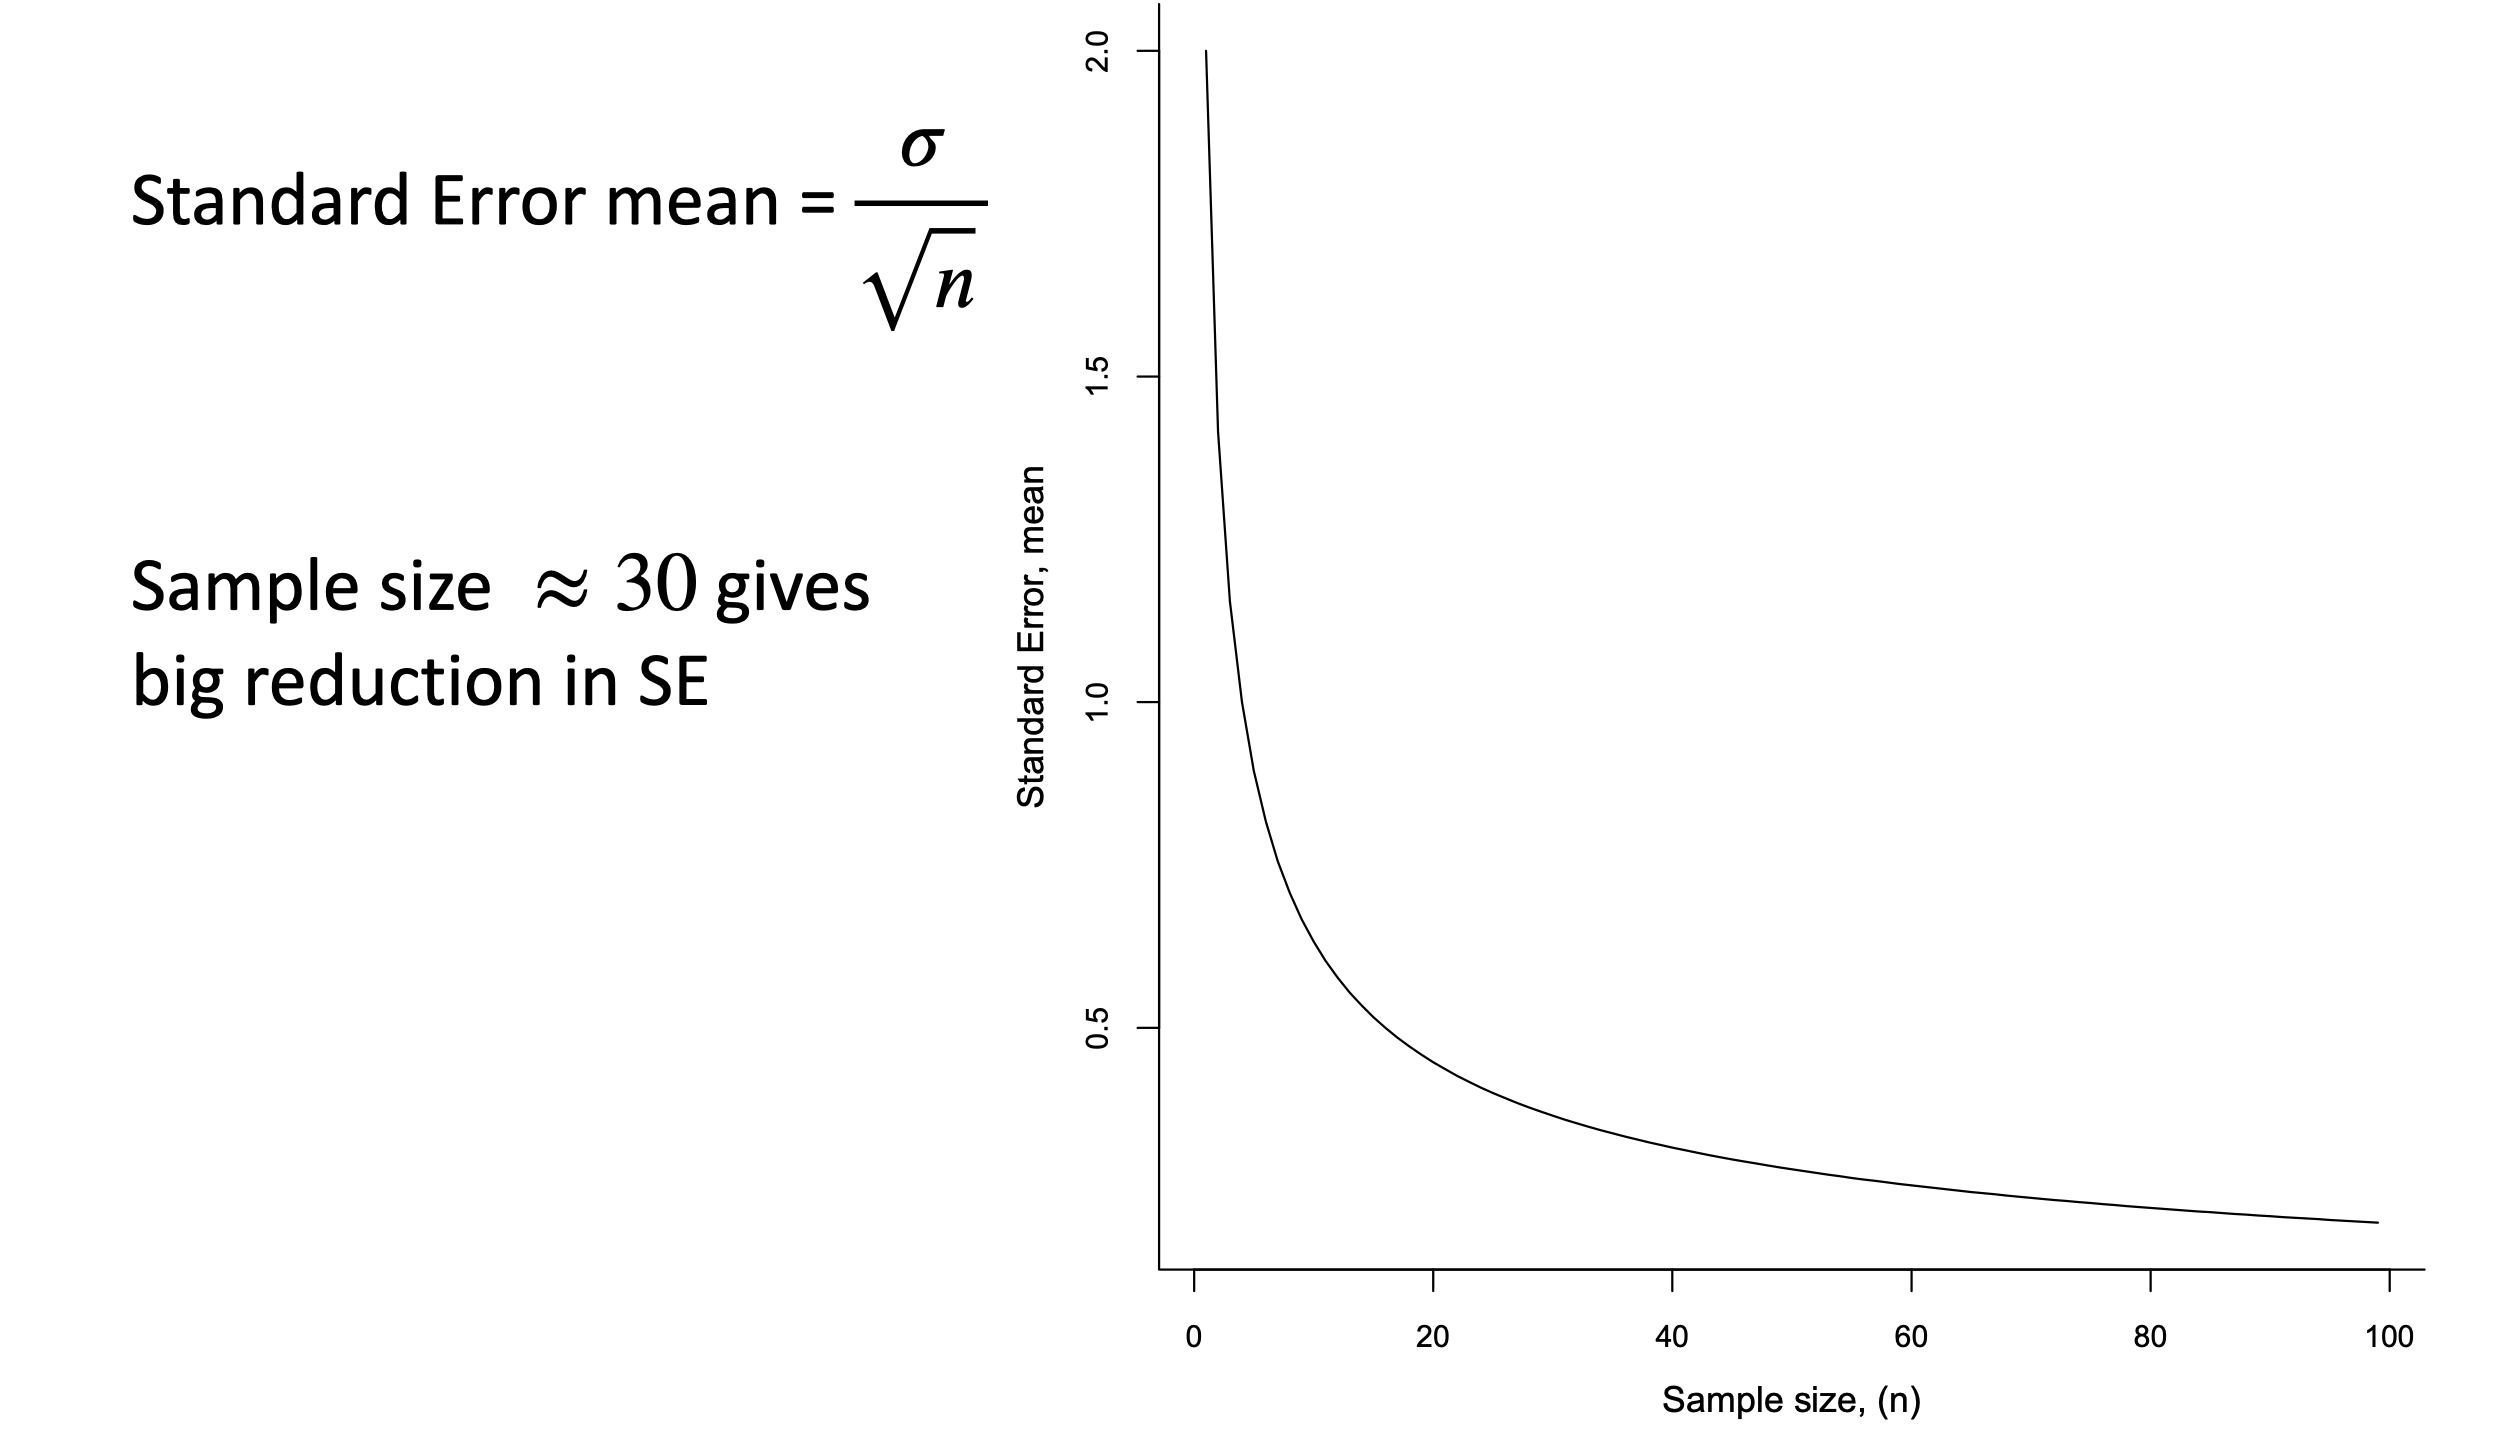
\includegraphics[width=34.86in]{images/Standard_Error}

\hypertarget{se-of-a-difference-and-balance.}{%
\subsection{SE of a Difference and Balance.}\label{se-of-a-difference-and-balance.}}

Interestingly, we often are estimating the standard error of a difference. Remember the t-test? The test statstic is all about the difference between the means. We need a precise estimate of that difference to assess whether the null hypothesis (the differene = 0) can be rejected or not.

The standard error of a difference behaves differently, however.

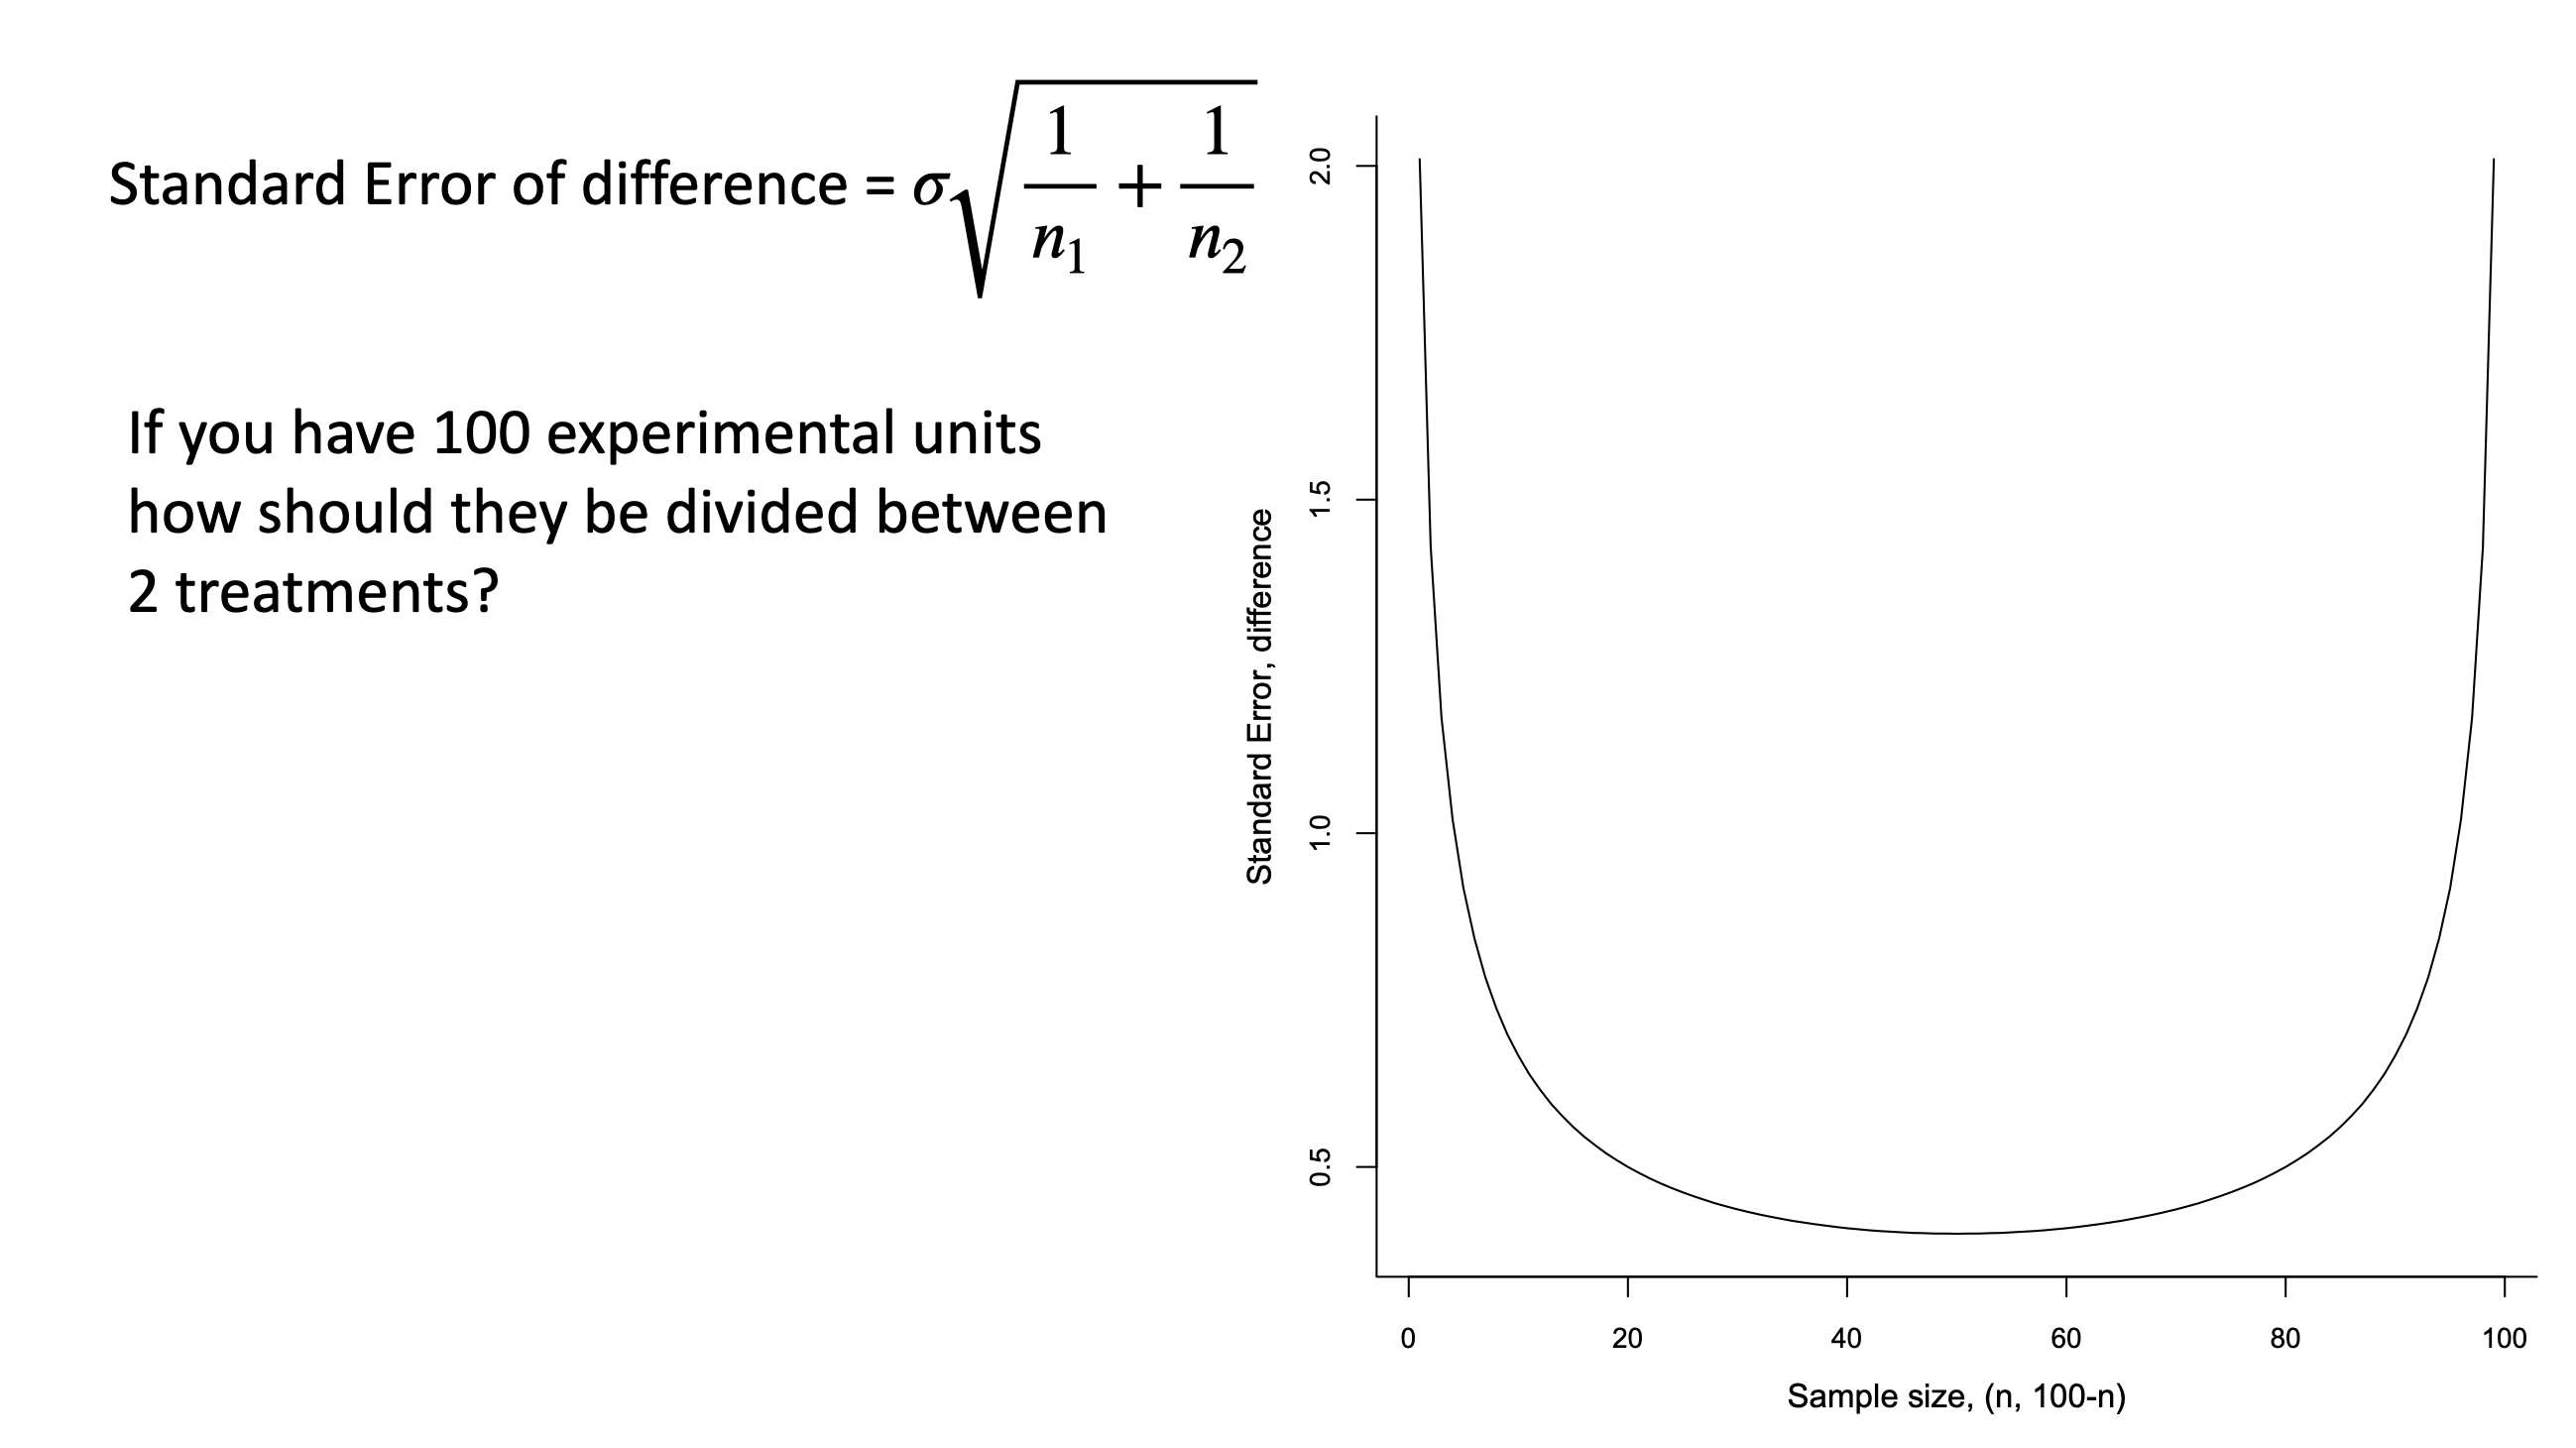
\includegraphics[width=36.08in]{images/SE2}

What this suggests is that we allocate our sample sizes in a balanced manner - 50\% to each group/treatment level. In general balanced designs are good -- equal numbers of replicates per treatment.

\hypertarget{however-sometimes-unbalanced-designs-are-better.}{%
\subsection{However sometimes unbalanced designs are better.}\label{however-sometimes-unbalanced-designs-are-better.}}

Say we have g treatments one of which is a control, say treatment 1, and we want to compare each of the other treatments with the control, so treatment 2 vs Control, treatment 3 vs Control, treatment 4 vs Control, etc. Then as we compare everything with the control we want more replicates of the control. The best allocation is \(n_{c} = n_{t}\sqrt{(g-1)}\)
where \(n_{t}\) is the number of replicates in the non-control treatment.

\hypertarget{the-crd-completely-randomised-design}{%
\section{The CRD: Completely Randomised Design}\label{the-crd-completely-randomised-design}}

Against this backdrop of understanding \textbf{randomisation} and \textbf{replication}, the most basic design is the Completely Randomized Design:

We have g treatment levels to compare (e.g.~Hot, Warm, Cold) and N units to use in our experiment. For a completely randomized design:

\begin{enumerate}
\def\labelenumi{\arabic{enumi}.}
\tightlist
\item
  Select sample sizes \(n_{1}, n_{2}, . . . , n_{g} = N\). Often we set the n's to be equal so we have a balanced design.
\item
  Choose \(n_{1}\) units at random to receive treatment 1, \(n_{2}\) units at random from the N − n1 remaining to receive treatment 2, and so on.
\end{enumerate}

\hypertarget{examples-and-challenge-questions}{%
\chapter{Examples and Challenge Questions}\label{examples-and-challenge-questions}}

In this section, we will review a field based experimental design example. There are challenge questions to answer.

We will also introduce tools to generate randomised experimental designs - this is a good trick to have up your sleeves!

\hypertarget{designing-your-first-experiment}{%
\section{Designing your first experiment}\label{designing-your-first-experiment}}

You are challenged to design an Arctic field manipulation experiment to evalauate UV-B radiation and increased CO2 impacts on plant growth.

Context: an arctic tundra study
Increasing ultraviolet-B (+UV-B) radiation from ozone depletion (the arctic ozone hole)
Increasing atmospheric CO2 (+CO2) from anthropogenic emissions
For plants: +UV-B potentially harmful, +CO2 potentially beneficial

Hypotheses
Elevated (+) UV-B radiation will reduce the growth of arctic plants
Elevated (+) \(CO_{2}\) will increase the growth of arctic plants

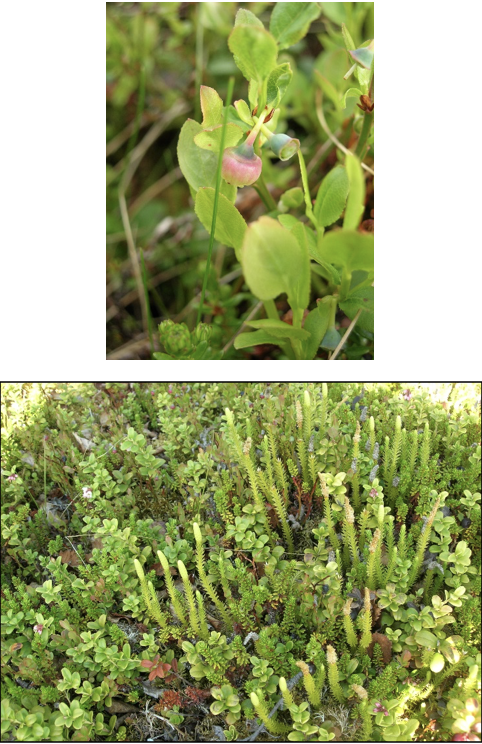
\includegraphics[width=6.69in]{images/ArcticPlants}

The resources available to you are constrained. The arctic research station has given permission for 16 plots (each 2m x 2m) in the natural vegetation nearby.

One +UV-B plot (2m x 2m) costs £4000 (this provides the UV-B lamps, frame, power and control system, wooden walkways around the plots)
One \(+CO_{2}\) plot (2m x 2m) costs £6000 (this provides a CO2 release system, CO2 control and covers CO2 purchase costs, wooden walkways around the plots)
One control plot (2m x 2m) costs £200 (marking posts, wooden walkways around the plots)

You have a budget of £61,000

Design an experiment to test the hypotheses (i.e.~the design of the plots and treatments including replication, not what measurements you will take - which will be plant growth rates\ldots.). Think hard about this. How many treatments do you have? How many plots/treatment would you like to allocate? Is this possible? Will this be a balanced design, given your max budget? If it isn't, what rule can you use to allocate them replicates to treatments?

Write an answer down, before moving to the next section. We'll provide the answer separately!

\hypertarget{using-r-to-generate-experimental-designs}{%
\section{Using R to generate Experimental Designs}\label{using-r-to-generate-experimental-designs}}

This is the place to stop for a moment and organise your R-course life. My suggestion is to do the following.

Create an Experimental Design folder on your computer. Put a data folder inside that. Use RStudio to create an RStudio Project file inside the Experimental Design folder. This will be the only place you need to focus for this mini-module.

Now, let's set up a script to do build this experimental design and actually generate soome data and do an analysis.

As with every script last semester, we start with a preamble and some libraries

\begin{Shaded}
\begin{Highlighting}[]
\CommentTok{\# Designing experiments with R: and introduction}
\CommentTok{\# MY NAME}
\CommentTok{\# DATE}

\CommentTok{\#libraries I need}

\FunctionTok{library}\NormalTok{(tidyverse)}
\FunctionTok{library}\NormalTok{(ggfortify)}
\FunctionTok{library}\NormalTok{(agricolae)}
\FunctionTok{library}\NormalTok{(car)}
\FunctionTok{library}\NormalTok{(gmodels)}
\FunctionTok{library}\NormalTok{(visreg)}
\end{Highlighting}
\end{Shaded}

That's alot of packages, but you'll see how we use them for designing and then analysing data.

To design and experiment, we are going to use the \texttt{design.csd} function from the \emph{agricolae} package, which we used last term to help with the tukey tests. It does WAY MORE!

This package has a great online help resource: \url{https://myaseen208.github.io/agricolae/articles/Intro_agricolae.html}

\begin{Shaded}
\begin{Highlighting}[]
\CommentTok{\# use this to make sure the random allocation pattern created for the design is the same for you and me}
\FunctionTok{set.seed}\NormalTok{(}\DecValTok{123}\NormalTok{)}

\CommentTok{\# define the treatments}
\NormalTok{treatments }\OtherTok{\textless{}{-}} \FunctionTok{c}\NormalTok{(}\StringTok{"Control"}\NormalTok{,}\StringTok{"UVB"}\NormalTok{,}\StringTok{"CO2"}\NormalTok{)}

\CommentTok{\# define the design (this does some randomisation for you!)}
\NormalTok{design }\OtherTok{\textless{}{-}} \FunctionTok{design.crd}\NormalTok{(treatments, }\AttributeTok{r =} \FunctionTok{c}\NormalTok{(}\DecValTok{6}\NormalTok{,}\DecValTok{5}\NormalTok{,}\DecValTok{5}\NormalTok{), }\AttributeTok{serie =} \DecValTok{0}\NormalTok{)}

\CommentTok{\# view the design {-} note that the actual data are in $book}
\FunctionTok{glimpse}\NormalTok{(design)}
\end{Highlighting}
\end{Shaded}

\begin{verbatim}
## List of 2
##  $ parameters:List of 7
##   ..$ design: chr "crd"
##   ..$ trt   : chr [1:3] "Control" "UVB" "CO2"
##   ..$ r     : num [1:3] 5 6 5
##   ..$ serie : num 0
##   ..$ seed  : int 515190382
##   ..$ kinds : chr "Super-Duper"
##   ..$       : logi TRUE
##  $ book      :'data.frame':  16 obs. of  3 variables:
##   ..$ plots     : num [1:16] 1 2 3 4 5 6 7 8 9 10 ...
##   ..$ r         : int [1:16] 1 1 1 2 2 2 3 3 4 3 ...
##   ..$ treatments: chr [1:16] "UVB" "CO2" "Control" "UVB" ...
\end{verbatim}

\begin{Shaded}
\begin{Highlighting}[]
\CommentTok{\# grab that book}
\NormalTok{use\_design }\OtherTok{\textless{}{-}}\NormalTok{ design}\SpecialCharTok{$}\NormalTok{book}

\CommentTok{\# show the design}
\NormalTok{use\_design}
\end{Highlighting}
\end{Shaded}

\begin{verbatim}
##    plots r treatments
## 1      1 1        UVB
## 2      2 1        CO2
## 3      3 1    Control
## 4      4 2        UVB
## 5      5 2        CO2
## 6      6 2    Control
## 7      7 3        CO2
## 8      8 3        UVB
## 9      9 4        CO2
## 10    10 3    Control
## 11    11 4        UVB
## 12    12 4    Control
## 13    13 5    Control
## 14    14 6    Control
## 15    15 5        CO2
## 16    16 5        UVB
\end{verbatim}

Great scott! So, we have 16 plots and we've randomly allocated the set of treatments to these plots, with 6 controls, and 5 of the non-control treatments. This is just what we wanted.

Time to move on to the next chapter, but stick with this script! We will come back to this example later.

\hypertarget{design-and-analysis-of-experiments}{%
\chapter{Design and Analysis of Experiments}\label{design-and-analysis-of-experiments}}

In this section, we will design and experiment, make up data for the experiment, and analyse the experiment.

This is a very good process to go through - you will understand more fully how to generate randomisation in your experiments, and you will better understand how data that you collect is \emph{structured} - from where does variation come in your measurements.

Another way to think about this is to consider that we are learning how statistics looks at data you've collected. We are going to make up data, where we know the answer to the question. Then we are going to plot these data, and analyse them.

\hypertarget{example-one}{%
\section{Example one}\label{example-one}}

We are now going to cheat by generating artificial data we we don't have time to go run the experiment.

The experiment is about plant biomass yield under several herbicide treatments: a control and two herbicides, and a third treatment that is a placebo - applied water but no herbicide. The hypothesis is\ldots.?

Start a new section of your script (some hashes) called Herbicide Example.

Now, enter the following code in your script file, then run it.

\begin{Shaded}
\begin{Highlighting}[]
\CommentTok{\# set the random seed {-} this will ensure that your results and mine here are the same.}
\FunctionTok{set.seed}\NormalTok{(}\DecValTok{123}\NormalTok{)}

\CommentTok{\#treatment names we have a control and two herbicides, Herb3 is a placebo (applied water but no herbicide)}
\NormalTok{treat }\OtherTok{\textless{}{-}} \FunctionTok{c}\NormalTok{(}\StringTok{"Cont"}\NormalTok{,}\StringTok{"Herb1"}\NormalTok{,}\StringTok{"Herb2"}\NormalTok{,}\StringTok{"Placebo"}\NormalTok{)}

\CommentTok{\#number of replicates}
\NormalTok{Nreps }\OtherTok{\textless{}{-}} \DecValTok{30}

\CommentTok{\#Total number of experimental units}
\NormalTok{Total.units }\OtherTok{\textless{}{-}}\NormalTok{ Nreps }\SpecialCharTok{*} \FunctionTok{length}\NormalTok{(treat)}

\CommentTok{\#Our completely randomized design}
\CommentTok{\# not the trick of adding the $book at the end of the code}
\NormalTok{design }\OtherTok{\textless{}{-}} \FunctionTok{design.crd}\NormalTok{(treat, Nreps, }\AttributeTok{serie =} \DecValTok{0}\NormalTok{)}\SpecialCharTok{$}\NormalTok{book}

\CommentTok{\# check it out (the first 10 rows)}
\FunctionTok{head}\NormalTok{(design, }\DecValTok{10}\NormalTok{)}
\end{Highlighting}
\end{Shaded}

\begin{verbatim}
##    plots r   treat
## 1      1 1    Cont
## 2      2 1   Herb1
## 3      3 2   Herb1
## 4      4 1 Placebo
## 5      5 2 Placebo
## 6      6 3 Placebo
## 7      7 3   Herb1
## 8      8 2    Cont
## 9      9 1   Herb2
## 10    10 2   Herb2
\end{verbatim}

\hypertarget{making-up-data}{%
\subsection{Making up data}\label{making-up-data}}

Right, lets make up some artificial data so we know the right answers -- this is a very good way of checking you understand what's going on.

First, lets define some randon variation centred around 0 with a standard deviation of 3:

\begin{Shaded}
\begin{Highlighting}[]
\CommentTok{\#Our experimental errors, normal distribution mean = 0, standard deviation = 3}
\CommentTok{\# rnorm is random normal distribution {-} the bell curve!}
\NormalTok{error }\OtherTok{\textless{}{-}} \FunctionTok{rnorm}\NormalTok{(Total.units, }\AttributeTok{mean=}\DecValTok{0}\NormalTok{, }\AttributeTok{sd=}\DecValTok{3}\NormalTok{)}
\end{Highlighting}
\end{Shaded}

Now we need to actually generate a response variable. The thing we `measured'. For this experiment we are \emph{measuring} yield - the grams of dry biomass at the end of the experimental season.

To do this, we have to think about the mean of the yield (we'll set it to 20), the deviation caused by Herbicide 1 (+5 average yield), the deviation caused by Herbicide 2 (+6 average yield) and the deviation caused by the placebo (nothing) and the error among observations (error). If this works, there should be Controls and Placebos with values around 20, and Herbicide values around ±25-26. But keep in mind\ldots{} we have a standard deviation of 3 in the error\ldots{} what will that do? Let's see.

\begin{Shaded}
\begin{Highlighting}[]
\CommentTok{\#the observations of yield}
\NormalTok{design}\SpecialCharTok{$}\NormalTok{obs }\OtherTok{\textless{}{-}} 
  \CommentTok{\# mean yield Control}
  \DecValTok{20} \SpecialCharTok{+} 
  \CommentTok{\# deviation caused by Herbicide 1}
\NormalTok{  (design}\SpecialCharTok{$}\NormalTok{treat}\SpecialCharTok{==}\StringTok{"Herb1"}\NormalTok{) }\SpecialCharTok{*} \DecValTok{5} \SpecialCharTok{+} 
\NormalTok{  (design}\SpecialCharTok{$}\NormalTok{treat }\SpecialCharTok{==} \StringTok{"Herb2"}\NormalTok{) }\SpecialCharTok{*} \DecValTok{6} \SpecialCharTok{+} 
\NormalTok{  (design}\SpecialCharTok{$}\NormalTok{treat }\SpecialCharTok{==} \StringTok{"Placebo"}\NormalTok{)}\SpecialCharTok{*}\DecValTok{1} \SpecialCharTok{+}
\NormalTok{  error}

\CommentTok{\# look at it}
\NormalTok{design}\SpecialCharTok{$}\NormalTok{obs}
\end{Highlighting}
\end{Shaded}

\begin{verbatim}
##   [1] 25.56702 23.32992 23.39985 21.54529 20.96267 22.34314 24.19572 15.45247
##   [9] 28.25849 28.09586 25.03735 26.36961 20.44643 16.30186 25.99108 29.62076
##  [17] 24.05645 22.01011 25.48992 29.60826 25.83590 23.77995 21.06598 21.85137
##  [25] 19.10903 20.54631 21.71607 24.78175 15.84089 24.56500 26.21161 19.96028
##  [33] 16.21851 24.50682 17.80657 23.74981 30.64518 24.90522 27.33204 18.15174
##  [41] 13.41104 27.87253 19.64131 22.48390 25.17527 15.41037 16.58438 15.85613
##  [49] 20.56557 20.75066 19.84848 19.97868 22.47068 25.11759 25.55048 24.92058
##  [57] 18.45873 22.02616 23.09377 15.56172 26.78291 18.20024 21.20411 25.58635
##  [65] 25.67710 26.29930 22.20238 20.63010 30.71839 18.37104 29.64641 14.20080
##  [73] 30.80997 22.67665 29.92778 20.63348 21.45997 20.32328 25.25901 18.08680
##  [81] 18.75511 24.83941 27.00049 23.06356 27.87863 18.63813 16.75083 24.45870
##  [89] 19.76979 23.40537 21.49970 21.09057 18.48304 18.64256 23.66625 28.52046
##  [97] 18.82317 29.38274 22.55174 26.41338 25.95806 24.86078 21.90836 20.61218
## [105] 25.47680 21.99004 23.06115 20.40581 15.70540 23.30232 28.04868 18.26389
## [113] 30.76203 24.50311 19.17553 25.11028 26.65809 18.84203 26.01325 26.79324
\end{verbatim}

\begin{Shaded}
\begin{Highlighting}[]
\CommentTok{\# look at the design now.}
\FunctionTok{head}\NormalTok{(design)}
\end{Highlighting}
\end{Shaded}

\begin{verbatim}
##   plots r   treat      obs
## 1     1 1    Cont 25.56702
## 2     2 1   Herb1 23.32992
## 3     3 2   Herb1 23.39985
## 4     4 1 Placebo 21.54529
## 5     5 2 Placebo 20.96267
## 6     6 3 Placebo 22.34314
\end{verbatim}

\hypertarget{into-the-dplyr-and-ggplot-pipeline.}{%
\subsection{Into the dplyr and ggplot pipeline.}\label{into-the-dplyr-and-ggplot-pipeline.}}

Great stuff. Now we can move to our standard data management and visualisation pipeline.

\begin{enumerate}
\def\labelenumi{\arabic{enumi}.}
\tightlist
\item
  review the data
\item
  sumamrise the data with dplyr - generate means and se's for the treatments
\item
  visualise with ggplot2
\end{enumerate}

\begin{Shaded}
\begin{Highlighting}[]
\CommentTok{\# check the data}
\FunctionTok{glimpse}\NormalTok{(design)}
\end{Highlighting}
\end{Shaded}

\begin{verbatim}
## Rows: 120
## Columns: 4
## $ plots <dbl> 1, 2, 3, 4, 5, 6, 7, 8, 9, 10, 11, 12, 13, 14, 15, 16, 17, 18...
## $ r     <int> 1, 1, 2, 1, 2, 3, 3, 2, 1, 2, 3, 4, 4, 4, 5, 5, 6, 3, 5, 6, 7...
## $ treat <chr> "Cont", "Herb1", "Herb1", "Placebo", "Placebo", "Placebo", "H...
## $ obs   <dbl> 25.56702, 23.32992, 23.39985, 21.54529, 20.96267, 22.34314, 2...
\end{verbatim}

\begin{Shaded}
\begin{Highlighting}[]
\CommentTok{\# summarise to get means and ses}
\NormalTok{sumDat }\OtherTok{\textless{}{-}}\NormalTok{ design }\SpecialCharTok{\%\textgreater{}\%} 
  \FunctionTok{group\_by}\NormalTok{(treat) }\SpecialCharTok{\%\textgreater{}\%} 
  \FunctionTok{summarise}\NormalTok{(}
    \AttributeTok{meanYield =} \FunctionTok{mean}\NormalTok{(obs),}
    \AttributeTok{seYield =} \FunctionTok{sd}\NormalTok{(obs)}\SpecialCharTok{/}\FunctionTok{sqrt}\NormalTok{(}\FunctionTok{n}\NormalTok{())}
\NormalTok{  )}
\end{Highlighting}
\end{Shaded}

\begin{verbatim}
## `summarise()` ungrouping output (override with `.groups` argument)
\end{verbatim}

\begin{Shaded}
\begin{Highlighting}[]
\CommentTok{\# plot the raw data and the mean±se}
\CommentTok{\# start with the mean±se and then add the raw data}
\FunctionTok{ggplot}\NormalTok{(sumDat, }\FunctionTok{aes}\NormalTok{(}\AttributeTok{x =}\NormalTok{ treat, }\AttributeTok{y =}\NormalTok{ meanYield))}\SpecialCharTok{+}
  \FunctionTok{geom\_point}\NormalTok{(}\AttributeTok{size =} \DecValTok{5}\NormalTok{)}\SpecialCharTok{+}
  \FunctionTok{geom\_errorbar}\NormalTok{(}\AttributeTok{data =}\NormalTok{ sumDat, }\FunctionTok{aes}\NormalTok{(}\AttributeTok{ymin =}\NormalTok{ meanYield }\SpecialCharTok{{-}}\NormalTok{ seYield, }\AttributeTok{ymax =}\NormalTok{ meanYield}\SpecialCharTok{+}\NormalTok{seYield),}
                \AttributeTok{width =} \FloatTok{0.1}\NormalTok{)}\SpecialCharTok{+}
  \FunctionTok{geom\_point}\NormalTok{(}\AttributeTok{data =}\NormalTok{ design, }\FunctionTok{aes}\NormalTok{(}\AttributeTok{x =}\NormalTok{ treat, }\AttributeTok{y =}\NormalTok{ obs), }\AttributeTok{colour =} \StringTok{\textquotesingle{}red\textquotesingle{}}\NormalTok{, }\AttributeTok{alpha =} \FloatTok{0.3}\NormalTok{)}
\end{Highlighting}
\end{Shaded}

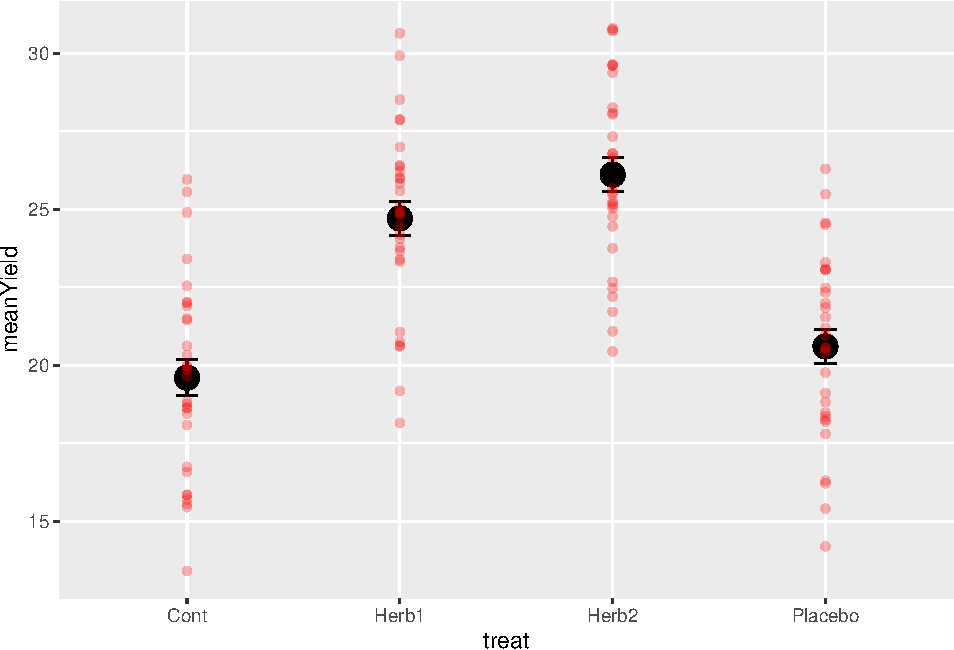
\includegraphics{Introduction-to-Experimental-Design-and-Analysis_files/figure-latex/unnamed-chunk-14-1.pdf}

A few things to notice.

\begin{enumerate}
\def\labelenumi{\arabic{enumi}.}
\tightlist
\item
  The data are quite variable and the means of the herbicide treatments are roughly 5 and 6 units higher. This is as we expected\ldots.
\item
  The standard errors are quite small! Why is that!?
\item
  For those of you interested in some extra reading and thinking, the 95\% Confidence Interval around the means can be calculated using \texttt{1.96*SE} == \texttt{1.96*sd(obs)/sqrt(n())}. Go ahead and do that and look into that if you want\ldots{}
\end{enumerate}

\hypertarget{the-one-way-anova.}{%
\section{The One-Way ANOVA.}\label{the-one-way-anova.}}

If you've been paying attention, we've essentially designed and plotted the data for a 1-way ANOVA. These data are very similar to the daphnia parasite data we finished semester 1 with.

To analyse these data, we use the \texttt{lm()} function to build the model, check assumptions, and then make inference. Let's go.

\begin{Shaded}
\begin{Highlighting}[]
\CommentTok{\# the model}
\NormalTok{modYield }\OtherTok{\textless{}{-}} \FunctionTok{lm}\NormalTok{(obs }\SpecialCharTok{\textasciitilde{}}\NormalTok{ treat, }\AttributeTok{data =}\NormalTok{ design)}

\CommentTok{\# assumptions}
\FunctionTok{autoplot}\NormalTok{(modYield)}
\end{Highlighting}
\end{Shaded}

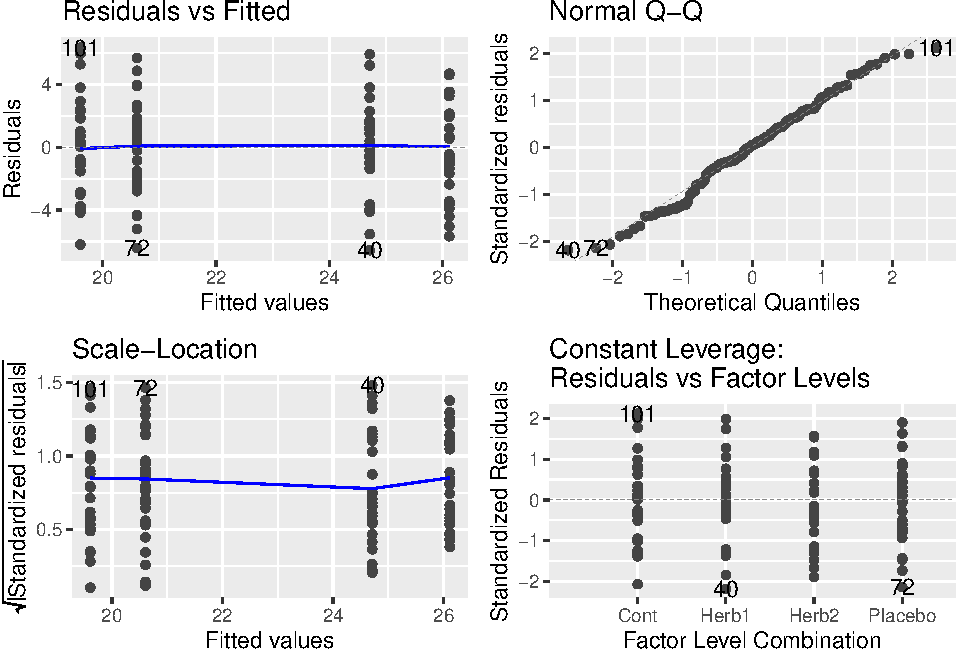
\includegraphics{Introduction-to-Experimental-Design-and-Analysis_files/figure-latex/unnamed-chunk-15-1.pdf}

\begin{Shaded}
\begin{Highlighting}[]
\CommentTok{\# inference: anova}
\FunctionTok{anova}\NormalTok{(modYield)}
\end{Highlighting}
\end{Shaded}

\begin{verbatim}
## Analysis of Variance Table
## 
## Response: obs
##            Df  Sum Sq Mean Sq F value    Pr(>F)    
## treat       3  888.39 296.129  31.968 3.905e-15 ***
## Residuals 116 1074.54   9.263                      
## ---
## Signif. codes:  0 '***' 0.001 '**' 0.01 '*' 0.05 '.' 0.1 ' ' 1
\end{verbatim}

\begin{Shaded}
\begin{Highlighting}[]
\CommentTok{\# contrasts}
\FunctionTok{summary}\NormalTok{(modYield)}
\end{Highlighting}
\end{Shaded}

\begin{verbatim}
## 
## Call:
## lm(formula = obs ~ treat, data = design)
## 
## Residuals:
##     Min      1Q  Median      3Q     Max 
## -6.5589 -1.8698  0.1395  2.0230  6.3494 
## 
## Coefficients:
##              Estimate Std. Error t value Pr(>|t|)    
## (Intercept)   19.6087     0.5557  35.288  < 2e-16 ***
## treatHerb1     5.1019     0.7858   6.492 2.18e-09 ***
## treatHerb2     6.5048     0.7858   8.277 2.43e-13 ***
## treatPlacebo   0.9993     0.7858   1.272    0.206    
## ---
## Signif. codes:  0 '***' 0.001 '**' 0.01 '*' 0.05 '.' 0.1 ' ' 1
## 
## Residual standard error: 3.044 on 116 degrees of freedom
## Multiple R-squared:  0.4526, Adjusted R-squared:  0.4384 
## F-statistic: 31.97 on 3 and 116 DF,  p-value: 3.905e-15
\end{verbatim}

\hypertarget{making-insight-and-inference}{%
\subsection{Making insight and inference}\label{making-insight-and-inference}}

Lets walks through things very discretely.

\begin{enumerate}
\def\labelenumi{\arabic{enumi}.}
\tightlist
\item
  Our graph suggests that herbicide treatments have an effect of increasing yield.
\item
  Our model is designed to test this hypothesis - are any of the differences among means non-zero?
\item
  Our hypothesis is probably really about whether the herbicide and placebos are differnt than the controls
\item
  Our diagnostics are fantistic\ldots{} the best you've ever seen.
\item
  The Anova Table confirms that there are differences - we can reject the null hypothesis
\item
  The summary table confirms that Herb1 and Herb2 are both larger than controls and the Placebo is not.
\end{enumerate}

How do we interpret even more? The estimate associated with Control is 20! Just where it should be.

The estimates associated with Herb1, Herb2 and Placebo are the differences between the mean of these treatments and the control (the reference level!). These differences are positive for Herb1 and Herb2, close to 5 and 6 respectively (as expected) and this positive difference is not 0 via the statistical test.

However, the differnce for Placebo is close to 0 and therefore we can not reject the null hypothesis test that it differs from control. GENUIS!

\hypertarget{a-priori-vs.-post-hoc-contrasts}{%
\section{A priori vs.~Post-Hoc Contrasts}\label{a-priori-vs.-post-hoc-contrasts}}

In the semester 1, we introduced how to do a Tukey Test.

This is known as an \emph{a posteriori} test -- testing the significance of things suggested by the experiment, also known as data snooping or data dredging. These are multiple comparison methods (Bonferroni, Scheffe method, Tukey honest significant difference, Duncan's multiple range test) which try to control the chance of getting a significant result by chance.

To understand the risks of these, consider this experimental design. We have 7 treatments. With 7 treatments, there are 21 pairwise comparisons. With p-value threshold of \(0.05\) we expect 1/20 (5/100) tests to be significant. So with this 7 treatment and 21 comparison design, would you expect a signficant result by chance? You betyja.

This is why, unless a priori (in advance) you can justify ALL pairwise comparisons, a tukey test may not be appropriate.

Some statisticians really don't like them ``In my view multiple comparison methods have no place at all in the interpretation of data'' Nelder (very well respected statistician).

\hypertarget{the-more-appropriate-approach.}{%
\subsection{The more appropriate approach.}\label{the-more-appropriate-approach.}}

The classical approach is to specify a priori (before experiment) a set of hypotheses then test them using contrasts. For our experiment, as noted above, we were probably interested in what our treatment contrasts provided - tests of difference with the control.

Specifying specific contrasts is easy once you get your head around the `structure' of the syntax. Lets have a go with specifying a comparison JUST between Herbicide 1 and the control.

\begin{Shaded}
\begin{Highlighting}[]
\CommentTok{\# check the levels and ORDERING of the treatments}
\FunctionTok{levels}\NormalTok{(design}\SpecialCharTok{$}\NormalTok{treat)}
\end{Highlighting}
\end{Shaded}

\begin{verbatim}
## NULL
\end{verbatim}

\begin{Shaded}
\begin{Highlighting}[]
\CommentTok{\# define the contrast you want using {-}1, 1 and 0\textquotesingle{}s}
\CommentTok{\# this says compare control with herbicide 1.... and ignore the Herb2 and Placebo}
\CommentTok{\# we give the reference {-}1 and the \textquotesingle{}other\textquotesingle{} 1.}
\NormalTok{contrast }\OtherTok{\textless{}{-}} \FunctionTok{c}\NormalTok{(}\SpecialCharTok{{-}}\DecValTok{1}\NormalTok{,}\DecValTok{1}\NormalTok{,}\DecValTok{0}\NormalTok{,}\DecValTok{0}\NormalTok{)}

\CommentTok{\# use the fit.contrast function from gmodels}
\FunctionTok{fit.contrast}\NormalTok{(modYield, }\StringTok{"treat"}\NormalTok{, contrast)}
\end{Highlighting}
\end{Shaded}

\begin{verbatim}
##                      Estimate Std. Error  t value     Pr(>|t|)
## treat c=( -1 1 0 0 ) 5.101935  0.7858436 6.492304 2.181992e-09
## attr(,"class")
## [1] "fit_contrast"
\end{verbatim}

\begin{Shaded}
\begin{Highlighting}[]
\CommentTok{\# remind ourselves of the contrast from the summary table}
\FunctionTok{summary}\NormalTok{(modYield)}
\end{Highlighting}
\end{Shaded}

\begin{verbatim}
## 
## Call:
## lm(formula = obs ~ treat, data = design)
## 
## Residuals:
##     Min      1Q  Median      3Q     Max 
## -6.5589 -1.8698  0.1395  2.0230  6.3494 
## 
## Coefficients:
##              Estimate Std. Error t value Pr(>|t|)    
## (Intercept)   19.6087     0.5557  35.288  < 2e-16 ***
## treatHerb1     5.1019     0.7858   6.492 2.18e-09 ***
## treatHerb2     6.5048     0.7858   8.277 2.43e-13 ***
## treatPlacebo   0.9993     0.7858   1.272    0.206    
## ---
## Signif. codes:  0 '***' 0.001 '**' 0.01 '*' 0.05 '.' 0.1 ' ' 1
## 
## Residual standard error: 3.044 on 116 degrees of freedom
## Multiple R-squared:  0.4526, Adjusted R-squared:  0.4384 
## F-statistic: 31.97 on 3 and 116 DF,  p-value: 3.905e-15
\end{verbatim}

\begin{quote}
Notice that the results are the same from the summary(modYield) and the fit.contrast.
\end{quote}

If we want to compare the two herbicides we can use this approach. Note in advance that this contrast DOES NOT exist in the summary table!

\begin{Shaded}
\begin{Highlighting}[]
\CommentTok{\# define the contrast you want using {-}1, 1 and 0\textquotesingle{}s}
\CommentTok{\# this says compare herb1 with herb2, ignoring the control and placebo.}
\CommentTok{\# we give the reference {-}1 and the \textquotesingle{}other\textquotesingle{} 1.}
\NormalTok{contrast }\OtherTok{\textless{}{-}} \FunctionTok{c}\NormalTok{(}\DecValTok{0}\NormalTok{,}\SpecialCharTok{{-}}\DecValTok{1}\NormalTok{,}\DecValTok{1}\NormalTok{,}\DecValTok{0}\NormalTok{)}

\CommentTok{\# use the fit.contrast function from gmodels}
\FunctionTok{fit.contrast}\NormalTok{(modYield, }\StringTok{"treat"}\NormalTok{, contrast)}
\end{Highlighting}
\end{Shaded}

\begin{verbatim}
##                      Estimate Std. Error  t value   Pr(>|t|)
## treat c=( 0 -1 1 0 ) 1.402879  0.7858436 1.785189 0.07684408
## attr(,"class")
## [1] "fit_contrast"
\end{verbatim}

Isn't this cool? Note that the difference reported is the difference between the two means:

\begin{Shaded}
\begin{Highlighting}[]
\CommentTok{\# check our summary data}
\NormalTok{sumDat}
\end{Highlighting}
\end{Shaded}

\begin{verbatim}
## # A tibble: 4 x 3
##   treat   meanYield seYield
##   <chr>       <dbl>   <dbl>
## 1 Cont         19.6   0.580
## 2 Herb1        24.7   0.545
## 3 Herb2        26.1   0.546
## 4 Placebo      20.6   0.552
\end{verbatim}

Here it is: \(26.2 - 24.2 = 2\)

This says that despite the difference we created of \textasciitilde1 unit of yield between Herb1 and Herb2, when we defined error and generated the data, it created a significant difference detectable with statistics.

\hypertarget{comparing-the-average-of-the-herbicide-effect-with-the-control.}{%
\subsection{comparing the average of the herbicide effect with the control.}\label{comparing-the-average-of-the-herbicide-effect-with-the-control.}}

This might be a comparison you intended to make also\ldots{} the average effect of herbicides in general. To do this, we expand the idea of -1,1 and 0's to include 1/2s (and yes, 1/3's and more are possible):

\begin{Shaded}
\begin{Highlighting}[]
\CommentTok{\# define the contrast you want using {-}1, 1 and 0\textquotesingle{}s}
\CommentTok{\# this says compare control with the average of herbicide 1 and 2, ignoring the placebo}
\CommentTok{\# we give the reference {-}1 and the \textquotesingle{}other two\textquotesingle{} a 1/2 each.}
\NormalTok{contrast }\OtherTok{\textless{}{-}} \FunctionTok{c}\NormalTok{(}\SpecialCharTok{{-}}\DecValTok{1}\NormalTok{,}\DecValTok{1}\SpecialCharTok{/}\DecValTok{2}\NormalTok{,}\DecValTok{1}\SpecialCharTok{/}\DecValTok{2}\NormalTok{,}\DecValTok{0}\NormalTok{)}

\CommentTok{\# use the fit.contrast function from gmodels}
\FunctionTok{fit.contrast}\NormalTok{(modYield, }\StringTok{"treat"}\NormalTok{, contrast)}
\end{Highlighting}
\end{Shaded}

\begin{verbatim}
##                          Estimate Std. Error  t value     Pr(>|t|)
## treat c=( -1 0.5 0.5 0 ) 5.803375  0.6805605 8.527346 6.484593e-14
## attr(,"class")
## [1] "fit_contrast"
\end{verbatim}

Again, checking sumDat

\begin{Shaded}
\begin{Highlighting}[]
\NormalTok{sumDat}
\end{Highlighting}
\end{Shaded}

\begin{verbatim}
## # A tibble: 4 x 3
##   treat   meanYield seYield
##   <chr>       <dbl>   <dbl>
## 1 Cont         19.6   0.580
## 2 Herb1        24.7   0.545
## 3 Herb2        26.1   0.546
## 4 Placebo      20.6   0.552
\end{verbatim}

\((24.2+26.2)/2 = 25.2\) --\textgreater{} \(25.2 - 20 = 5.2\)

\hypertarget{writing-this-up}{%
\subsection{writing this up\ldots{}}\label{writing-this-up}}

Fill in these blanks using the various contrasts you made above!

\begin{quote}
We conclude that herbicides on average cause an \_\_\_\_\_ gram increase in yield (t = \_\_\_ , p = \_\_\_ ). We also note that there was a significant difference of \_\_\_\_\_ grams between the herbicides (t = \_\_\_\_\_ p = \_\_\_\_\_\_). The additional placebo treatment had no effect on yield (t = \_\_\_\_\_\_\_ p = \_\_\_\_\_\_\_\_\_\_).
\end{quote}

\hypertarget{randomized-complete-block-design-rcb}{%
\chapter{Randomized Complete Block design (RCB)}\label{randomized-complete-block-design-rcb}}

Blocking allows us to reduce the experimental error.

A block is a group of experimental units that are homogeneous in some sense -- in the same place, or measured at the same time, or by the same person. So when constructing blocks we try and select experimental units that are homogeneous within blocks but units in different blocks may be dissimilar.

Why block? When we use a completely randomised design, the location or timing of our treatment `plots' (patches, incubators, locations in a 96 well plate) can generate heterogeneity in experimental error (variation). As the variance of the Experimental Error increases, confidence intervals get wider and the power of our analysis decreases - it's harder to detect effects of our treatments against the background noise. Ideally we would like to use experimental units that are homogeneous so the experimental error will be small. Blocking does this.

The simplest blocked design is the \textbf{Randomized Complete Block design (RCB)}

We have one complete set of treatments in each block. Say you have g Treatments and r Blocks then the total number of experimental units is?

In the first block, we randomly assign the g treatments to the n units; we do an independent randomization, assigning treatments to units in each of the other blocks. This is the RCB design.

For example, consider the following matrix: the rows are the blocks, the letters the different treatments. In each block, each treatment is represented, but it is in a different location in the block (randomisation of the g treatments in the n units). The blocks are in a sequence - left to right - this could be different days, different locations or different positions on a hillside, for example representing an elevation or soil moisture gradient.

The Blocks are designed to `capture' that underlying source of variability and allow us to detect among treatment differences more effectively.

\begin{verbatim}
##      [,1] [,2] [,3] [,4] [,5]
## [1,] "A"  "B"  "A"  "E"  "D" 
## [2,] "C"  "A"  "D"  "C"  "A" 
## [3,] "D"  "E"  "B"  "D"  "C" 
## [4,] "E"  "C"  "E"  "B"  "E" 
## [5,] "B"  "D"  "C"  "A"  "B"
\end{verbatim}

It is important to note that blocks exist at the time of the randomization of treatments to units. We cannot impose blocking structure on a completely randomized design after the fact; either the randomization was blocked or it was not.

We use an RCB to increase the power and precision of an experiment by decreasing the error variance. This decrease in error variance is achieved by finding groups of units that are homogeneous (blocks) and, in effect, repeating the experiment independently in the different blocks. The RCB is an effective design when there is a single source of extraneous variation in the responses that we can identify ahead of time and use to partition the units into blocks.

In short ALWAYS block your experiment, if you can.

You can have spatial blocks, or temporal blocks where you repeat the experiment at different times, or block by batch.

In general, any source of variation that you think may influence the response and which can be identified prior to the experiment is a candidate for blocking.

\hypertarget{an-example-of-the-rcbd}{%
\section{An example of the RCBD}\label{an-example-of-the-rcbd}}

Lets modify our previous example to including blocking. Start another section with some \#\# and call it Blocking Example.

Of course, if you want to start another script, you can, but make sure you include all of the library()'s again!

\begin{Shaded}
\begin{Highlighting}[]
\CommentTok{\#Randomised Complete Block Design}

\CommentTok{\# ensure allocation is the same}
\FunctionTok{set.seed}\NormalTok{(}\DecValTok{123}\NormalTok{)}

\CommentTok{\# define the treatments}
\NormalTok{treat }\OtherTok{\textless{}{-}} \FunctionTok{c}\NormalTok{(}\StringTok{"Control"}\NormalTok{,}\StringTok{"Herb1"}\NormalTok{,}\StringTok{"Herb2"}\NormalTok{,}\StringTok{"Placebo"}\NormalTok{)}

\CommentTok{\# define the number of blocks}
\NormalTok{Nblocks }\OtherTok{\textless{}{-}} \DecValTok{5}

\CommentTok{\# consider this}
\NormalTok{Total.units }\OtherTok{\textless{}{-}}\NormalTok{ Nblocks }\SpecialCharTok{*} \FunctionTok{length}\NormalTok{(treat)}

\CommentTok{\# build the design}
\NormalTok{design }\OtherTok{\textless{}{-}} \FunctionTok{design.rcbd}\NormalTok{(treat, Nblocks, }\AttributeTok{serie =} \DecValTok{0}\NormalTok{)}\SpecialCharTok{$}\NormalTok{book}

\CommentTok{\# look at it}
\NormalTok{design}
\end{Highlighting}
\end{Shaded}

\begin{verbatim}
##    plots block   treat
## 1     11     1 Placebo
## 2     12     1 Control
## 3     13     1   Herb2
## 4     14     1   Herb1
## 5     21     2 Control
## 6     22     2   Herb1
## 7     23     2   Herb2
## 8     24     2 Placebo
## 9     31     3   Herb2
## 10    32     3   Herb1
## 11    33     3 Control
## 12    34     3 Placebo
## 13    41     4 Control
## 14    42     4   Herb2
## 15    43     4 Placebo
## 16    44     4   Herb1
## 17    51     5 Placebo
## 18    52     5 Control
## 19    53     5   Herb1
## 20    54     5   Herb2
\end{verbatim}

This is like the matrix above, but in tidy format! Excellent. This is how a block design looks in tidy-land.

Now, lets generate some data again.

\begin{Shaded}
\begin{Highlighting}[]
\CommentTok{\# set seed again ... }
\FunctionTok{set.seed}\NormalTok{(}\DecValTok{123}\NormalTok{)}

\CommentTok{\# define the error {-} note how we use the variable Total.units to get the number of observations}
\NormalTok{error }\OtherTok{\textless{}{-}} \FunctionTok{rnorm}\NormalTok{(Total.units, }\AttributeTok{mean =} \DecValTok{0}\NormalTok{, }\AttributeTok{sd =} \DecValTok{1}\NormalTok{) }\CommentTok{\# is this more or less variation than before?}

\CommentTok{\# generate the observations}
\CommentTok{\# note that we are now generating larger differences (10 and 9) among treatments}
\CommentTok{\# e.g. Herb1 is 10 units larger than the control.}
\NormalTok{design}\SpecialCharTok{$}\NormalTok{obs }\OtherTok{\textless{}{-}} \DecValTok{20} \SpecialCharTok{+} 
\NormalTok{  (design}\SpecialCharTok{$}\NormalTok{treat}\SpecialCharTok{==}\StringTok{"Herb1"}\NormalTok{) }\SpecialCharTok{*} \DecValTok{10} \SpecialCharTok{+} 
\NormalTok{  (design}\SpecialCharTok{$}\NormalTok{treat }\SpecialCharTok{==} \StringTok{"Herb2"}\NormalTok{) }\SpecialCharTok{*} \DecValTok{9} \SpecialCharTok{+} 
\NormalTok{  (design}\SpecialCharTok{$}\NormalTok{treat }\SpecialCharTok{==} \StringTok{"Placebo"}\NormalTok{) }\SpecialCharTok{*} \DecValTok{1} \SpecialCharTok{+} 
  \CommentTok{\# note that we are defining variation among blocks here}
  \CommentTok{\# block 1 is on average 10 units higher.... and block 5 is...}
\NormalTok{  (design}\SpecialCharTok{$}\NormalTok{block}\SpecialCharTok{==}\DecValTok{1}\NormalTok{) }\SpecialCharTok{*} \DecValTok{10} \SpecialCharTok{{-}}\NormalTok{ (design}\SpecialCharTok{$}\NormalTok{block}\SpecialCharTok{==}\DecValTok{5}\NormalTok{) }\SpecialCharTok{*} \DecValTok{10} \SpecialCharTok{+} 
\NormalTok{  error}

\FunctionTok{head}\NormalTok{(design, }\DecValTok{10}\NormalTok{)}
\end{Highlighting}
\end{Shaded}

\begin{verbatim}
##    plots block   treat      obs
## 1     11     1 Placebo 31.18707
## 2     12     1 Control 31.99603
## 3     13     1   Herb2 41.29937
## 4     14     1   Herb1 41.12746
## 5     21     2 Control 21.08111
## 6     22     2   Herb1 30.56917
## 7     23     2   Herb2 28.09290
## 8     24     2 Placebo 21.02990
## 9     31     3   Herb2 27.44097
## 10    32     3   Herb1 30.29749
\end{verbatim}

\hypertarget{analysing-the-crbd}{%
\section{Analysing the CRBD}\label{analysing-the-crbd}}

I'll leave it to you now to generate the following picture of the means ± standard errors.

This requires thinking hard about the use of dplyr tools (\texttt{group\_by()} and \texttt{summarise()}) and ggplot (adding more than one layer from two different sources of data - the summary data and the raw data).

Can you see our generation of block 1 and 5's variation?

\begin{verbatim}
## Rows: 20
## Columns: 4
## $ plots <dbl> 11, 12, 13, 14, 21, 22, 23, 24, 31, 32, 33, 34, 41, 42, 43, 4...
## $ block <fct> 1, 1, 1, 1, 2, 2, 2, 2, 3, 3, 3, 3, 4, 4, 4, 4, 5, 5, 5, 5
## $ treat <fct> Placebo, Control, Herb2, Herb1, Control, Herb1, Herb2, Placeb...
## $ obs   <dbl> 31.18707, 31.99603, 41.29937, 41.12746, 21.08111, 30.56917, 2...
\end{verbatim}

\begin{verbatim}
## `summarise()` ungrouping output (override with `.groups` argument)
\end{verbatim}

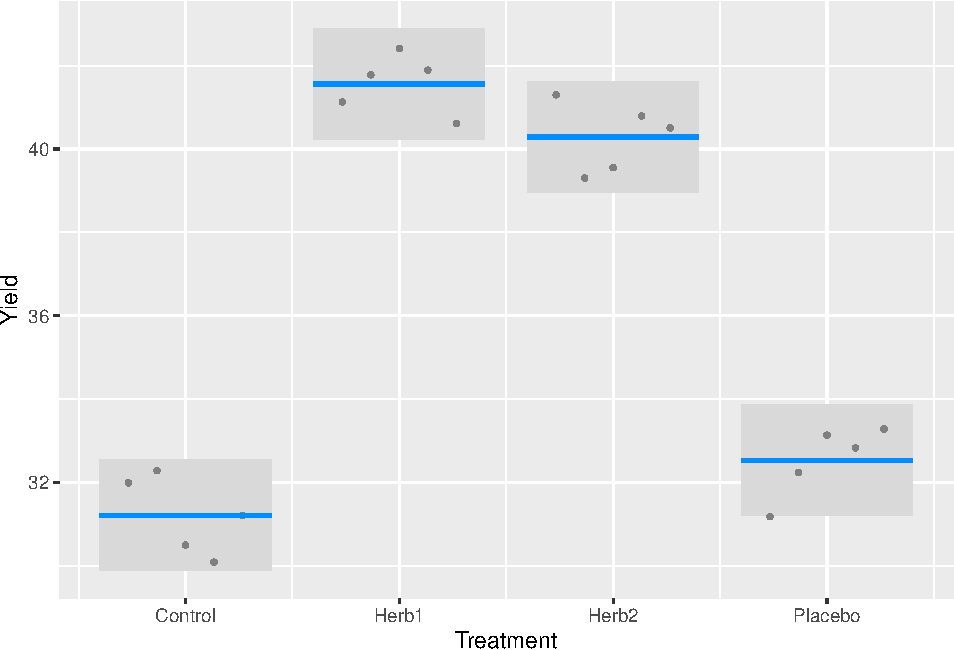
\includegraphics{Introduction-to-Experimental-Design-and-Analysis_files/figure-latex/unnamed-chunk-25-1.pdf}

\hypertarget{building-the-model}{%
\subsection{Building the model}\label{building-the-model}}

In order to understand what's going on with blocking, and it's importance, lets build the naive model that ignores block - treating this as a CRB - and the correct model, letting block absorb some of the variation.

\begin{Shaded}
\begin{Highlighting}[]
\CommentTok{\# models}
\NormalTok{naive\_model }\OtherTok{\textless{}{-}} \FunctionTok{lm}\NormalTok{(obs }\SpecialCharTok{\textasciitilde{}}\NormalTok{ treat, design)}
\NormalTok{block\_model }\OtherTok{\textless{}{-}} \FunctionTok{lm}\NormalTok{(obs }\SpecialCharTok{\textasciitilde{}}\NormalTok{ block }\SpecialCharTok{+}\NormalTok{ treat, design) }\CommentTok{\# note the order is important}

\CommentTok{\# anova tables}
\FunctionTok{anova}\NormalTok{(naive\_model)}
\end{Highlighting}
\end{Shaded}

\begin{verbatim}
## Analysis of Variance Table
## 
## Response: obs
##           Df Sum Sq Mean Sq F value  Pr(>F)  
## treat      3 417.82 139.274  2.5085 0.09579 .
## Residuals 16 888.34  55.521                  
## ---
## Signif. codes:  0 '***' 0.001 '**' 0.01 '*' 0.05 '.' 0.1 ' ' 1
\end{verbatim}

\begin{Shaded}
\begin{Highlighting}[]
\FunctionTok{anova}\NormalTok{(block\_model)}
\end{Highlighting}
\end{Shaded}

\begin{verbatim}
## Analysis of Variance Table
## 
## Response: obs
##           Df Sum Sq Mean Sq F value    Pr(>F)    
## block      4 877.08 219.270  233.68 2.871e-11 ***
## treat      3 417.82 139.274  148.43 9.469e-10 ***
## Residuals 12  11.26   0.938                      
## ---
## Signif. codes:  0 '***' 0.001 '**' 0.01 '*' 0.05 '.' 0.1 ' ' 1
\end{verbatim}

The first important thing to focus on here is the difference in the Mean Sq Residual Errors - in the \texttt{naive\_model}, it is \(55.52\). In the \texttt{block\_model}, it is \(0.94\).

The second important thing to notice is that haveing allocated variation to block in the \texttt{block\_model}, and thus reducing the error variation, the \emph{treatment} effect shifts from being insignificant to significant.

\hypertarget{are-the-estimates-of-the-parameters-what-we-expect}{%
\subsection{Are the estimates of the parameters what we expect?}\label{are-the-estimates-of-the-parameters-what-we-expect}}

Lets check that the model is estimating differences as we might have expected. We can do this using the summary table.

Let's remember that, for example, the mean of Herb1 is expected to be 10 units higher than control with a yield of 20, and block 1 is supposed to be \textasciitilde10 units higher than 2,3,4.

\begin{Shaded}
\begin{Highlighting}[]
\FunctionTok{summary}\NormalTok{(block\_model)}
\end{Highlighting}
\end{Shaded}

\begin{verbatim}
## 
## Call:
## lm(formula = obs ~ block + treat, data = design)
## 
## Residuals:
##     Min      1Q  Median      3Q     Max 
## -1.3505 -0.7196  0.2147  0.6396  1.0719 
## 
## Coefficients:
##              Estimate Std. Error t value Pr(>|t|)    
## (Intercept)   31.2184     0.6126  50.957 2.14e-15 ***
## block2       -11.2092     0.6850 -16.365 1.43e-09 ***
## block3       -12.1132     0.6850 -17.685 5.84e-10 ***
## block4       -11.3415     0.6850 -16.558 1.25e-09 ***
## block5       -20.8449     0.6850 -30.433 9.94e-13 ***
## treatHerb1    10.3450     0.6126  16.886 9.96e-10 ***
## treatHerb2     9.0721     0.6126  14.808 4.50e-09 ***
## treatPlacebo   1.3192     0.6126   2.153   0.0523 .  
## ---
## Signif. codes:  0 '***' 0.001 '**' 0.01 '*' 0.05 '.' 0.1 ' ' 1
## 
## Residual standard error: 0.9687 on 12 degrees of freedom
## Multiple R-squared:  0.9914, Adjusted R-squared:  0.9864 
## F-statistic: 197.1 on 7 and 12 DF,  p-value: 2.009e-11
\end{verbatim}

In this table, the \emph{INTERCEPT} is specifying the \textbf{FIRST BLOCK} and the \textbf{CONTROL TREATMENT LEVEL} - we know this because it's these words that are missing from the rest of the table, and they are each the first alphanumerially in the list of blocks and treatments.

The value of the control, block 1 is approximately 30! Which is 20+10, which is what we expected.
The value of Herb1 is \textasciitilde10 units higher than this (remember, the value 9.84 is the DIFFERENCE between the control and treatment)
And the value of block 5 is reported as 20 unites lower than block 1 control. This too is correct because, as above, block 1 control is 10 units higher than the control mean (20+10) and block 5 10 unites lower\ldots. Make sure you get this logic!

The take home message here is that these numbers make complete sense with respect to what we simulated, and controlling for the among block variation gave us more power to detect a treatment effect, something we would have missed had we not estimated the block source of variation.

\hypertarget{correct-standard-errors-for-a-figure}{%
\subsection{Correct Standard Errors for a Figure}\label{correct-standard-errors-for-a-figure}}

When we made our initial plot above, we calculated the standard error based on all observations among blocks. However, the variation we really wish to represent is the variation after having controlled for the blocking effects.

This means that the standard deviation we should probably use is of the error variance from the correct model: \(0.94\).

The standard deviation is the \(\sqrt{Var}\) and thus, our correct standard errors from the model are \(\sqrt{0.94}\)

There is a very nice plotting function in the package \emph{visreg} that delivers these proper standard errors in a nice ggplot framework. It presents points are partial residuals (deviation from the mean for each replicate), lines depciting the means, and shaded area as a 95\% confidence interval, calculated 1.96*SE, where the SE is estimated from the model error variance (just above). Compare this to your first graph.

\begin{Shaded}
\begin{Highlighting}[]
\FunctionTok{visreg}\NormalTok{(block\_model, }\StringTok{"treat"}\NormalTok{, }\AttributeTok{gg=}\ConstantTok{TRUE}\NormalTok{)}\SpecialCharTok{+}
  \FunctionTok{ylab}\NormalTok{(}\StringTok{"Yield"}\NormalTok{) }\SpecialCharTok{+} 
  \FunctionTok{xlab}\NormalTok{(}\StringTok{"Treatment"}\NormalTok{) }
\end{Highlighting}
\end{Shaded}

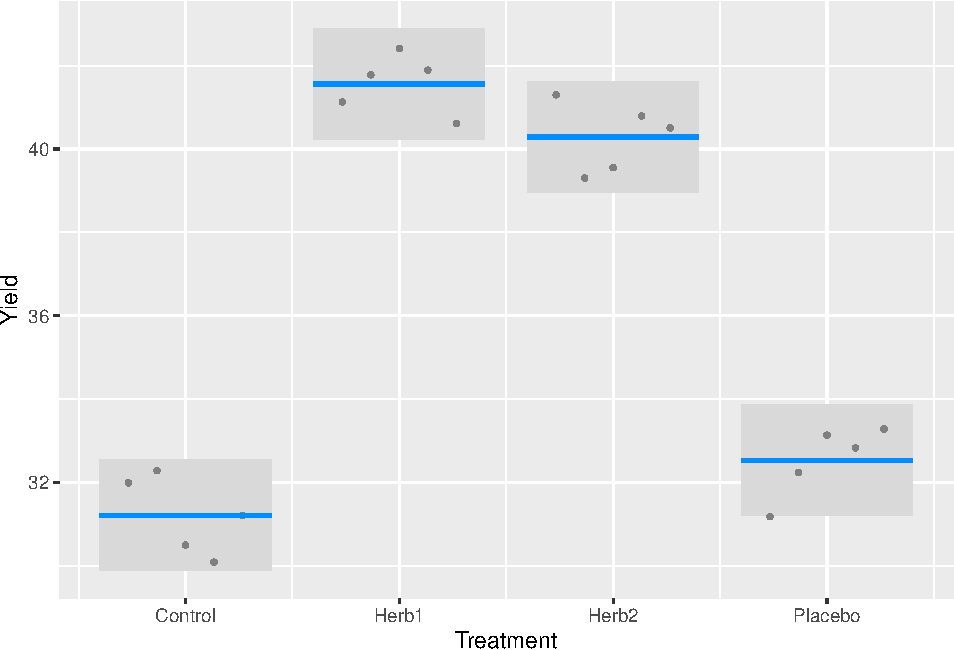
\includegraphics{Introduction-to-Experimental-Design-and-Analysis_files/figure-latex/unnamed-chunk-28-1.pdf}

\hypertarget{making-inference-confidence-intervals-and-contrasts}{%
\subsection{Making inference: confidence intervals and contrasts}\label{making-inference-confidence-intervals-and-contrasts}}

We are now in a very strong position to make inference.

Let's start with a rule of thumb linked to the 95\% confidence interval. If the CIs don't overlap, they are different; if they do, they are not. This indicates that Cont and Placebo are not significantly different (95\% confidence intervals overlap). Herb1 and Herb 2 are significantly different from these, but not each other.

This is OK. But it's not robust. Let's revisit our \emph{post-hoc} and \emph{a priori} methods for evaluating differnces among treatments. We can apply a tukey test and calculate all pairwise differences. This is not a good idea, but let's do it.

\begin{Shaded}
\begin{Highlighting}[]
\CommentTok{\# use agricolae HSD.test()}

\NormalTok{tukey\_out }\OtherTok{\textless{}{-}} \FunctionTok{HSD.test}\NormalTok{(block\_model, }\StringTok{"treat"}\NormalTok{, }\AttributeTok{group =} \ConstantTok{TRUE}\NormalTok{)}
\NormalTok{tukey\_out}\SpecialCharTok{$}\NormalTok{groups}
\end{Highlighting}
\end{Shaded}

\begin{verbatim}
##              obs groups
## Herb1   30.46167      a
## Herb2   29.18874      a
## Placebo 21.43581      b
## Control 20.11665      b
\end{verbatim}

This confirms our intuition and 95\% Confidence Interval insights. But is it correct?

Let's make a formal test of one of the pairwise tests that looks obvious - between Herb1 and Herb2

\begin{Shaded}
\begin{Highlighting}[]
\CommentTok{\# fit.contrast from gmodels package}
\NormalTok{contrast }\OtherTok{\textless{}{-}} \FunctionTok{c}\NormalTok{(}\DecValTok{0}\NormalTok{,}\SpecialCharTok{{-}}\DecValTok{1}\NormalTok{,}\DecValTok{1}\NormalTok{,}\DecValTok{0}\NormalTok{)}
\FunctionTok{fit.contrast}\NormalTok{(block\_model, }\StringTok{"treat"}\NormalTok{, contrast)}
\end{Highlighting}
\end{Shaded}

\begin{verbatim}
##                       Estimate Std. Error   t value   Pr(>|t|)
## treat c=( 0 -1 1 0 ) -1.272934  0.6126423 -2.077777 0.05985811
## attr(,"class")
## [1] "fit_contrast"
\end{verbatim}

Amazing. The contrast defining a specific test provides a different answer than the post-hoc Tukey test and our guess based on the 95\% CIs. Why is that? Which is right?

Of course the contrast is the correct and most reliable result. While both \emph{fit.contrast} and \emph{HSD.test} both manage the model complexity and variance estimates properly, only the contrast reduces the probability of finding a significant difference by chance or failing to find one.

\hypertarget{the-latin-square-design-lsd}{%
\chapter{The Latin Square Design (LSD)}\label{the-latin-square-design-lsd}}

Sometimes you will have two sources of variation in space or time, or perhaps space and time. Perhaps there is a gradient of elevation up and down a hillside, and a gradient of sun incidence orthoganol (90˚) to that. There are innumerable examples one could imagine. The principle is that in an LSD, the treatments are allocated randomly in `rows' and `columns'.

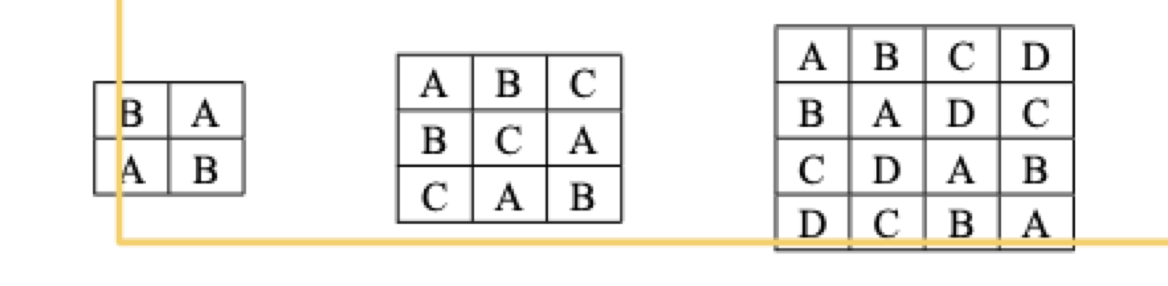
\includegraphics[width=16.22in]{images/lsd}

A Latin Square blocks on both rows and columns simultaneously.

Agricolae has a built in function for helping generate these designs, obvio. Again, new section or new script\ldots..

\begin{Shaded}
\begin{Highlighting}[]
\CommentTok{\# makes sure random allocation happens the same for everyone.}
\FunctionTok{set.seed}\NormalTok{(}\DecValTok{123}\NormalTok{)}

\CommentTok{\#}
\NormalTok{treat}\OtherTok{\textless{}{-}} \FunctionTok{c}\NormalTok{(}\StringTok{"Cont"}\NormalTok{,}\StringTok{"Herb1"}\NormalTok{,}\StringTok{"Herb2"}\NormalTok{,}\StringTok{"Placebo"}\NormalTok{)}

\CommentTok{\# design.lsd}
\NormalTok{design }\OtherTok{\textless{}{-}} \FunctionTok{design.lsd}\NormalTok{(treat,}\AttributeTok{serie =} \DecValTok{0}\NormalTok{)}\SpecialCharTok{$}\NormalTok{book}
\NormalTok{design}
\end{Highlighting}
\end{Shaded}

\begin{verbatim}
##    plots row col   treat
## 1     11   1   1    Cont
## 2     12   1   2   Herb1
## 3     13   1   3   Herb2
## 4     14   1   4 Placebo
## 5     21   2   1   Herb1
## 6     22   2   2   Herb2
## 7     23   2   3 Placebo
## 8     24   2   4    Cont
## 9     31   3   1 Placebo
## 10    32   3   2    Cont
## 11    33   3   3   Herb1
## 12    34   3   4   Herb2
## 13    41   4   1   Herb2
## 14    42   4   2 Placebo
## 15    43   4   3    Cont
## 16    44   4   4   Herb1
\end{verbatim}

Make sure you understand that the double-blocking has happened! See the figure above with 4 letters. Can you create on a piece of paper the matrix from this design you've made in R?

Now, lets generate some data, as before.

\begin{Shaded}
\begin{Highlighting}[]
\CommentTok{\# for fun, set again.}
\FunctionTok{set.seed}\NormalTok{(}\DecValTok{123}\NormalTok{)}

\NormalTok{Total.units }\OtherTok{\textless{}{-}} \FunctionTok{length}\NormalTok{(treat) }\SpecialCharTok{*} \FunctionTok{length}\NormalTok{(treat)}
\NormalTok{error }\OtherTok{\textless{}{-}} \FunctionTok{rnorm}\NormalTok{(Total.units,}\DecValTok{0}\NormalTok{,}\DecValTok{1}\NormalTok{)}

\CommentTok{\# make sure you think about where we generated variation in the blocking!}
\NormalTok{design}\SpecialCharTok{$}\NormalTok{obs }\OtherTok{\textless{}{-}} \DecValTok{20} \SpecialCharTok{+} 
\NormalTok{  (design}\SpecialCharTok{$}\NormalTok{treat}\SpecialCharTok{==}\StringTok{"Herb1"}\NormalTok{) }\SpecialCharTok{*} \DecValTok{10} \SpecialCharTok{+} 
\NormalTok{  (design}\SpecialCharTok{$}\NormalTok{treat }\SpecialCharTok{==} \StringTok{"Herb2"}\NormalTok{) }\SpecialCharTok{*} \DecValTok{9} \SpecialCharTok{+}               
\NormalTok{  (design}\SpecialCharTok{$}\NormalTok{row}\SpecialCharTok{==}\DecValTok{1}\NormalTok{) }\SpecialCharTok{*} \DecValTok{10} \SpecialCharTok{{-}}\NormalTok{ (design}\SpecialCharTok{$}\NormalTok{col}\SpecialCharTok{==}\DecValTok{4}\NormalTok{) }\SpecialCharTok{*} \DecValTok{10} \SpecialCharTok{+} 
\NormalTok{  error}

\CommentTok{\# look at it....  there are three explanatory variables... }
\CommentTok{\# treat, row{-}block, column{-}block!}
\FunctionTok{head}\NormalTok{(design)}
\end{Highlighting}
\end{Shaded}

\begin{verbatim}
##   plots row col   treat      obs
## 1    11   1   1    Cont 30.18707
## 2    12   1   2   Herb1 41.99603
## 3    13   1   3   Herb2 41.29937
## 4    14   1   4 Placebo 21.12746
## 5    21   2   1   Herb1 31.08111
## 6    22   2   2   Herb2 29.56917
\end{verbatim}

\hypertarget{fitting-the-model}{%
\subsection{Fitting the model}\label{fitting-the-model}}

Let's fit the naive and full models as before

\begin{Shaded}
\begin{Highlighting}[]
\NormalTok{naive\_lsd }\OtherTok{\textless{}{-}} \FunctionTok{lm}\NormalTok{(obs }\SpecialCharTok{\textasciitilde{}}\NormalTok{ treat, }\AttributeTok{data =}\NormalTok{ design)}
\NormalTok{full\_lsd }\OtherTok{\textless{}{-}} \FunctionTok{lm}\NormalTok{(obs }\SpecialCharTok{\textasciitilde{}}\NormalTok{ row }\SpecialCharTok{+}\NormalTok{ col }\SpecialCharTok{+}\NormalTok{ treat, }\AttributeTok{data =}\NormalTok{ design)}
\FunctionTok{anova}\NormalTok{(naive\_lsd)}
\end{Highlighting}
\end{Shaded}

\begin{verbatim}
## Analysis of Variance Table
## 
## Response: obs
##           Df Sum Sq Mean Sq F value Pr(>F)
## treat      3 398.31 132.771  2.2902 0.1303
## Residuals 12 695.68  57.973
\end{verbatim}

\begin{Shaded}
\begin{Highlighting}[]
\FunctionTok{anova}\NormalTok{(full\_lsd)}
\end{Highlighting}
\end{Shaded}

\begin{verbatim}
## Analysis of Variance Table
## 
## Response: obs
##           Df Sum Sq Mean Sq F value    Pr(>F)    
## row        3 402.44 134.145 139.002 6.209e-06 ***
## col        3 287.45  95.818  99.287 1.672e-05 ***
## treat      3 398.31 132.771 137.578 6.401e-06 ***
## Residuals  6   5.79   0.965                      
## ---
## Signif. codes:  0 '***' 0.001 '**' 0.01 '*' 0.05 '.' 0.1 ' ' 1
\end{verbatim}

Very quickly we can see, again, that without blocking, we have a risk of not detecting differences among treatments!

Take a look above at the \texttt{design\$obs} object. Can you review the \texttt{summary} output and validate that the model is estimating what we simulated?

\begin{Shaded}
\begin{Highlighting}[]
\FunctionTok{summary}\NormalTok{(full\_lsd)}
\end{Highlighting}
\end{Shaded}

\begin{verbatim}
## 
## Call:
## lm(formula = obs ~ row + col + treat, data = design)
## 
## Residuals:
##      Min       1Q   Median       3Q      Max 
## -0.99849 -0.41205  0.00493  0.37463  1.24126 
## 
## Coefficients:
##              Estimate Std. Error t value Pr(>|t|)    
## (Intercept)   30.7965     0.7766  39.654 1.72e-08 ***
## row2         -11.2092     0.6946 -16.137 3.60e-06 ***
## row3         -12.1132     0.6946 -17.438 2.28e-06 ***
## row4         -11.3415     0.6946 -16.327 3.36e-06 ***
## col2           1.2130     0.6946   1.746    0.131    
## col3           0.4538     0.6946   0.653    0.538    
## col4          -9.1817     0.6946 -13.218 1.16e-05 ***
## treatHerb1    10.2526     0.6946  14.759 6.08e-06 ***
## treatHerb2     9.1602     0.6946  13.187 1.17e-05 ***
## treatPlacebo  -0.4739     0.6946  -0.682    0.521    
## ---
## Signif. codes:  0 '***' 0.001 '**' 0.01 '*' 0.05 '.' 0.1 ' ' 1
## 
## Residual standard error: 0.9824 on 6 degrees of freedom
## Multiple R-squared:  0.9947, Adjusted R-squared:  0.9868 
## F-statistic: 125.3 on 9 and 6 DF,  p-value: 3.921e-06
\end{verbatim}

Finally, we can use contrasts to test a few of our key hypotheses. Make some notes on what these things mean!

\begin{Shaded}
\begin{Highlighting}[]
\CommentTok{\#first the set of comparisons with control}
\NormalTok{contrast1 }\OtherTok{\textless{}{-}} \FunctionTok{rbind}\NormalTok{(}
  \StringTok{"C v H1"} \OtherTok{=} \FunctionTok{c}\NormalTok{(}\SpecialCharTok{{-}}\DecValTok{1}\NormalTok{,}\DecValTok{1}\NormalTok{,}\DecValTok{0}\NormalTok{,}\DecValTok{0}\NormalTok{),}
  \StringTok{"C v H2"} \OtherTok{=} \FunctionTok{c}\NormalTok{(}\SpecialCharTok{{-}}\DecValTok{1}\NormalTok{,}\DecValTok{0}\NormalTok{,}\DecValTok{1}\NormalTok{,}\DecValTok{0}\NormalTok{),}
  \StringTok{"C v P"} \OtherTok{=} \FunctionTok{c}\NormalTok{(}\SpecialCharTok{{-}}\DecValTok{1}\NormalTok{,}\DecValTok{0}\NormalTok{,}\DecValTok{0}\NormalTok{,}\DecValTok{1}\NormalTok{))}

\FunctionTok{fit.contrast}\NormalTok{(full\_lsd, }\StringTok{"treat"}\NormalTok{, contrast1)}
\end{Highlighting}
\end{Shaded}

\begin{verbatim}
##               Estimate Std. Error    t value     Pr(>|t|)
## treatC v H1 10.2525618  0.6946426 14.7594771 6.079845e-06
## treatC v H2  9.1601564  0.6946426 13.1868620 1.174267e-05
## treatC v P  -0.4738879  0.6946426 -0.6822038 5.205624e-01
## attr(,"class")
## [1] "fit_contrast"
\end{verbatim}

\begin{Shaded}
\begin{Highlighting}[]
\CommentTok{\# now the H1 vs H2}
\NormalTok{contrast2 }\OtherTok{\textless{}{-}} \FunctionTok{rbind}\NormalTok{(}\StringTok{"H1 v H2"} \OtherTok{=} \FunctionTok{c}\NormalTok{(}\DecValTok{0}\NormalTok{,}\SpecialCharTok{{-}}\DecValTok{1}\NormalTok{,}\DecValTok{1}\NormalTok{,}\DecValTok{0}\NormalTok{))}
\FunctionTok{fit.contrast}\NormalTok{(full\_lsd, }\StringTok{"treat"}\NormalTok{, contrast2)}
\end{Highlighting}
\end{Shaded}

\begin{verbatim}
##               Estimate Std. Error   t value  Pr(>|t|)
## treatH1 v H2 -1.092405  0.6946426 -1.572615 0.1668691
## attr(,"class")
## [1] "fit_contrast"
\end{verbatim}

\hypertarget{designs-for-testing-for-interactions-factorial-designs.}{%
\chapter{Designs for testing for interactions: factorial designs.}\label{designs-for-testing-for-interactions-factorial-designs.}}

\hypertarget{introducing-interactions}{%
\section{Introducing Interactions}\label{introducing-interactions}}

Before jumping into an example, let's introduce a simple statement that forms the core of both asking and interpreting \emph{interactions}.

If there is an interaction between two explanatory variables, X and Z, on our response variable Y, then:

\begin{quote}
The effect of X on Y varies by Z. \textbf{OR} The effect of X on Y depends on Z.
\end{quote}

This use of \emph{varies by} \textbf{OR} \emph{depends on} defines context dependency and that's what defines interactions.

Now, let's return to our CO2 and UV-B solar radiation experiment in the Arctic Tundra example to introduce the idea of an interaction again.

Context: an arctic tundra study
Increasing ultraviolet-B (+UV-B) radiation from ozone depletion (the arctic ozone hole)
Increasing atmospheric CO2 (+CO2) from anthropogenic emissions
For plants: UV-B potentially harmful, +CO2 potentially beneficial
Therefore +CO2 could alleviate UV-B damage impacts.

Hypotheses
+UV-B radiation will reduce the growth of arctic plants
+CO2 will increase the growth of arctic plants
+UV-B radiation impacts will be less under +CO2

What is unique about these context and hypotheses? It's the presentation of CO2 and UVB in the same statement and the use of words like ``the effect of X will alleviate the impacts of Y'' and words like ``the effects of X will be less under Y''. These words and phrases reflect the context dependency of the effects of treatment levels.

Thus, to restate what we introduced above\ldots. when we talk about interactions, we can rely on a very simple vocabulary that is independent of the actual treatment levels: we can always describe an interaction like this:

\begin{quote}
The effect of X on Y depends on Z.
\end{quote}

or

\begin{quote}
The effect of X on Y varies by Z.
\end{quote}

In this `rubric', Y is the response variable, and X and Z are explanatory, independent variables. So, in our example above,

\begin{quote}
the effect of CO2 on plant biomass yield depends on UV-B radiation levels.
\end{quote}

OR

\begin{quote}
the effect of CO2 on plant biomass yield varies with UV-B radiation levels.
\end{quote}

This simple phrasing describes any interaction.

Here are some numerical examples to drive home the point.

Control = 20g Yield
UV-B = 10g Yield
C02 = 29g Yield

ADDITIVE RESULT: C02 + UV-B = 39g Yield
SYNERGISTIC RESULT: C02 + UV-B = 60g Yield
ANTAGONISTIC RESULT: C02 + UV-B = 19g Yield

\hypertarget{lets-design-an-experiment-again}{%
\subsection{Let's design an experiment, again\ldots{}}\label{lets-design-an-experiment-again}}

Your resources:

The arctic research station has given permission for 16 plots (each 2m x 2m) in the natural vegetation nearby.
- One UV-B plot (2m x 2m) costs £4000 (this provides the UV-B lamps, frame, power and control system, wooden walkways around the plots)
- One CO2 plot (2m x 2m) costs £6000 (this provides a CO2 release system, CO2 control and covers CO2 purchase costs, wooden walkways around the plots)
- One control plot (2m x 2m) costs £200 (marking posts, wooden walkways around the plots)
- Yes, the CO2 supply system does fit underneath the UV-B lamps.

You have a budget of £86,000

Design an experiment to test the hypotheses. (An answer is on the BB Site)

\hypertarget{the-factorial-design-how-and-why-study-interactions}{%
\subsection{The Factorial Design: How and Why Study Interactions?}\label{the-factorial-design-how-and-why-study-interactions}}

The UV-B and C02 experiment could be thought of as two experiments a Control vs UV-B and a Control vs C02 experiment. If we combine these we get a Factorial Experiment where the treatments are

\begin{itemize}
\tightlist
\item
  Control
\item
  UV-B
\item
  C02
\item
  UV-B + C02
\end{itemize}

So we have all combinations of treatments.

But do we treat each of these as unique treatments (e.g.~the one-way ANOVA example)? No, we don't. We design and analyse the data we collect in a two-way analysis - a factorial design. Two-way ANOVA (and ANCOVA - see later), are the toolboxes.

Factorial treatments have two main advantages. When factors \emph{DO interact} -- so the effect of C02 depends on UV-B -- then we can estimate the interaction - the dependency. \emph{One-way designs} cannot do this, and can lead to serious misunderstandings (because we are assuming that the effect of one thing DOES NOT depend on the other).

Furthermore, when factors \emph{DON'T interact}, \emph{factorial designs} are more efficient (smaller error variance) than one-way designs experiments.

Hence ALWAYS use factorial designs when you can!

\hypertarget{a-factorial-design-and-the-two-way-anova}{%
\section{A Factorial Design and the Two-Way ANOVA}\label{a-factorial-design-and-the-two-way-anova}}

I'd recommend a new script now for this section. It's a pretty distinct example. Don't forget to use library() at the top to get all those packages working for this script. And don't forget, this script can live in the same R Project as the other one(s).

\begin{Shaded}
\begin{Highlighting}[]
\FunctionTok{set.seed}\NormalTok{(}\DecValTok{123}\NormalTok{)}

\NormalTok{Nreps }\OtherTok{\textless{}{-}} \DecValTok{4} \CommentTok{\# 4 replicates per treatment level}
\NormalTok{trt }\OtherTok{\textless{}{-}} \FunctionTok{c}\NormalTok{(}\DecValTok{2}\NormalTok{,}\DecValTok{2}\NormalTok{) }\CommentTok{\# sets out the 2{-}way design}
\NormalTok{design }\OtherTok{\textless{}{-}} \FunctionTok{design.ab}\NormalTok{(trt,}\AttributeTok{r=}\NormalTok{Nreps,}\AttributeTok{serie=}\DecValTok{0}\NormalTok{,}\AttributeTok{design=}\StringTok{"crd"}\NormalTok{)}\SpecialCharTok{$}\NormalTok{book}
\FunctionTok{head}\NormalTok{(design)}
\end{Highlighting}
\end{Shaded}

\begin{verbatim}
##   plots r A B
## 1     1 1 2 1
## 2     2 1 1 2
## 3     3 1 1 1
## 4     4 1 2 2
## 5     5 2 2 2
## 6     6 2 2 1
\end{verbatim}

So, the \texttt{design.ab} function generates a nice picture, but uses numbers instead of words for the various treatments and has set Letters as the treatments.

We don't support this approach - you WILL forget what the numbers and letters mean, so let's change these CODES to represent CO2 and UVB REALITY. We'll use \texttt{fct\_recode} from the tidyverse package called \texttt{forcats} (for categories, but we like cats).

\begin{Shaded}
\begin{Highlighting}[]
\NormalTok{design }\OtherTok{\textless{}{-}}\NormalTok{ design }\SpecialCharTok{\%\textgreater{}\%}
  \FunctionTok{rename}\NormalTok{(}\AttributeTok{UVB =}\NormalTok{ A, }\AttributeTok{CO2 =}\NormalTok{ B) }\SpecialCharTok{\%\textgreater{}\%} 
  \FunctionTok{mutate}\NormalTok{(}\AttributeTok{UVB =} \FunctionTok{fct\_recode}\NormalTok{(UVB, }\StringTok{"Con"} \OtherTok{=} \StringTok{"1"}\NormalTok{, }\StringTok{"UVB+"} \OtherTok{=} \StringTok{"2"}\NormalTok{),}
         \AttributeTok{CO2 =} \FunctionTok{fct\_recode}\NormalTok{(CO2, }\StringTok{"Con"} \OtherTok{=} \StringTok{"1"}\NormalTok{,}\StringTok{"CO2+"} \OtherTok{=} \StringTok{"2"}\NormalTok{))}

\FunctionTok{head}\NormalTok{(design, }\DecValTok{10}\NormalTok{) }\CommentTok{\# is this what you expect}
\end{Highlighting}
\end{Shaded}

\begin{verbatim}
##    plots r  UVB  CO2
## 1      1 1 UVB+  Con
## 2      2 1  Con CO2+
## 3      3 1  Con  Con
## 4      4 1 UVB+ CO2+
## 5      5 2 UVB+ CO2+
## 6      6 2 UVB+  Con
## 7      7 3 UVB+ CO2+
## 8      8 2  Con  Con
## 9      9 3  Con  Con
## 10    10 4  Con  Con
\end{verbatim}

\begin{quote}
NOTE 1: this is using the \texttt{fct\_recode} function from the \emph{forcats} package in the \emph{tidyverse} collection.
\end{quote}

\begin{quote}
NOTE 2: we used the design = ``crd'' argument to specify a completely randomised, 2-way factorial design\ldots{} you could make this a block design with the ``rcbd''\ldots. see the help file for \texttt{design.ab}
\end{quote}

\hypertarget{build-the-data}{%
\subsection{Build the Data}\label{build-the-data}}

Here we will build two sources of data - one that has NO INTERACTION, and one that DOES.

\begin{Shaded}
\begin{Highlighting}[]
\CommentTok{\#Sample Sizes and errors}
\NormalTok{Total.units }\OtherTok{\textless{}{-}} \DecValTok{2} \SpecialCharTok{*} \DecValTok{2} \SpecialCharTok{*}\NormalTok{ Nreps}
\NormalTok{error }\OtherTok{\textless{}{-}} \FunctionTok{rnorm}\NormalTok{(Total.units,}\DecValTok{0}\NormalTok{,}\DecValTok{3}\NormalTok{)}

\CommentTok{\# the data with no interaction}
\NormalTok{design}\SpecialCharTok{$}\NormalTok{obs }\OtherTok{\textless{}{-}} \DecValTok{20} \SpecialCharTok{{-}} 
\NormalTok{  (design}\SpecialCharTok{$}\StringTok{"UVB"}\SpecialCharTok{==}\StringTok{"UVB+"}\NormalTok{) }\SpecialCharTok{*} \DecValTok{10} \SpecialCharTok{+} 
\NormalTok{  (design}\SpecialCharTok{$}\StringTok{"CO2"} \SpecialCharTok{==} \StringTok{"CO2+"}\NormalTok{) }\SpecialCharTok{*} \DecValTok{9} \SpecialCharTok{+} 
\NormalTok{  error}

\CommentTok{\# the data with interaction}
\NormalTok{design}\SpecialCharTok{$}\NormalTok{obs2 }\OtherTok{\textless{}{-}} \DecValTok{20} \SpecialCharTok{{-}} 
\NormalTok{  (design}\SpecialCharTok{$}\StringTok{"UVB"}\SpecialCharTok{==}\StringTok{"UVB+"}\NormalTok{) }\SpecialCharTok{*} \DecValTok{10} \SpecialCharTok{+} 
\NormalTok{  (design}\SpecialCharTok{$}\StringTok{"CO2"} \SpecialCharTok{==} \StringTok{"CO2+"}\NormalTok{) }\SpecialCharTok{*} \DecValTok{9} \SpecialCharTok{+} 
  \CommentTok{\# when both are together add 8 more (synergy)}
\NormalTok{  ((design}\SpecialCharTok{$}\StringTok{"UVB"}\SpecialCharTok{==}\StringTok{"UVB+"}\NormalTok{) }\SpecialCharTok{\&}\NormalTok{ (design}\SpecialCharTok{$}\StringTok{"CO2"} \SpecialCharTok{==} \StringTok{"CO2+"}\NormalTok{)) }\SpecialCharTok{*} \DecValTok{8} \SpecialCharTok{+} 
\NormalTok{  error}

\FunctionTok{head}\NormalTok{(design)}
\end{Highlighting}
\end{Shaded}

\begin{verbatim}
##   plots r  UVB  CO2      obs     obs2
## 1     1 1 UVB+  Con 12.82805 12.82805
## 2     2 1  Con CO2+ 25.38908 25.38908
## 3     3 1  Con  Con 19.17974 19.17974
## 4     4 1 UVB+ CO2+ 25.85980 33.85980
## 5     5 2 UVB+ CO2+ 15.92984 23.92984
## 6     6 2 UVB+  Con  7.75704  7.75704
\end{verbatim}

\hypertarget{plot-the-data}{%
\subsection{Plot the data!}\label{plot-the-data}}

Here we combine some dplyr magic (calcuating means in each group - there are two grouping variables!), some ggplot magic (adding the lines connecting the means on top of the raw data) and the beauty of patchwork, the package for plot layouts. Don't forget to check that you've got all of the \texttt{library()} calls at the top of your script, and that you ran them!

\begin{Shaded}
\begin{Highlighting}[]
\CommentTok{\# No interaction summary}
\NormalTok{sumDat1 }\OtherTok{\textless{}{-}}\NormalTok{ design }\SpecialCharTok{\%\textgreater{}\%} 
  \FunctionTok{group\_by}\NormalTok{(UVB, CO2) }\SpecialCharTok{\%\textgreater{}\%} 
  \FunctionTok{summarise}\NormalTok{(}
    \AttributeTok{obs =} \FunctionTok{mean}\NormalTok{(obs)}
\NormalTok{  )}

\CommentTok{\# with interaction summary}
\NormalTok{sumDat2 }\OtherTok{\textless{}{-}}\NormalTok{ design }\SpecialCharTok{\%\textgreater{}\%} 
  \FunctionTok{group\_by}\NormalTok{(UVB, CO2) }\SpecialCharTok{\%\textgreater{}\%} 
  \FunctionTok{summarise}\NormalTok{(}
    \AttributeTok{obs2 =} \FunctionTok{mean}\NormalTok{(obs2)}
\NormalTok{  )}

\CommentTok{\# no interaction}
\NormalTok{p1 }\OtherTok{\textless{}{-}} \FunctionTok{ggplot}\NormalTok{(design, }\FunctionTok{aes}\NormalTok{(}\AttributeTok{x =}\NormalTok{ UVB, }\AttributeTok{y =}\NormalTok{ obs, }\AttributeTok{colour =}\NormalTok{ CO2, }\AttributeTok{shape =}\NormalTok{ CO2, }\AttributeTok{group =}\NormalTok{ CO2))}\SpecialCharTok{+}
  \FunctionTok{geom\_point}\NormalTok{()}\SpecialCharTok{+}
  \FunctionTok{geom\_line}\NormalTok{(}\AttributeTok{data =}\NormalTok{ sumDat1)}

\CommentTok{\# with interaction}
\NormalTok{p2 }\OtherTok{\textless{}{-}} \FunctionTok{ggplot}\NormalTok{(design, }\FunctionTok{aes}\NormalTok{(}\AttributeTok{x =}\NormalTok{ UVB, }\AttributeTok{y =}\NormalTok{ obs2, }\AttributeTok{colour =}\NormalTok{ CO2, }\AttributeTok{shape =}\NormalTok{ CO2, }\AttributeTok{group =}\NormalTok{ CO2))}\SpecialCharTok{+}
  \FunctionTok{geom\_point}\NormalTok{()}\SpecialCharTok{+}
  \FunctionTok{geom\_line}\NormalTok{(}\AttributeTok{data =}\NormalTok{ sumDat2)}

\NormalTok{p1}\SpecialCharTok{+}\NormalTok{p2}
\end{Highlighting}
\end{Shaded}

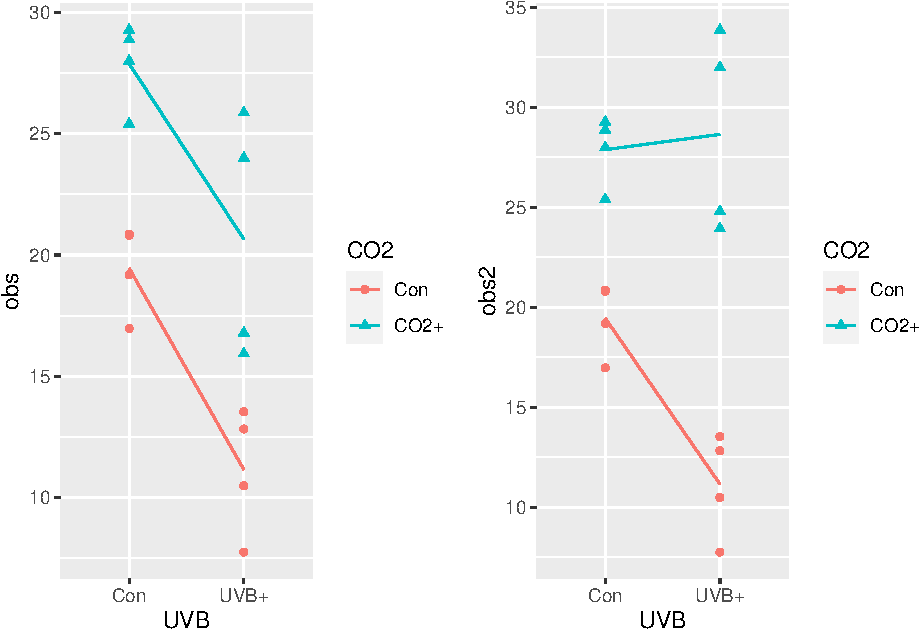
\includegraphics{Introduction-to-Experimental-Design-and-Analysis_files/figure-latex/unnamed-chunk-42-1.pdf}

What you see above on the left, is a pattern that suggest that the effect of \_\_\_\_\_\_ on \_\_\_\_\_\_\_\_ does not vary by \_\_\_\_\_\_\_\_. In contrast, on the right\ldots..:

\hypertarget{analyse-the-data}{%
\subsection{Analyse the data}\label{analyse-the-data}}

\begin{Shaded}
\begin{Highlighting}[]
\CommentTok{\# model with no interaction}
\NormalTok{int\_mod\_1 }\OtherTok{\textless{}{-}} \FunctionTok{lm}\NormalTok{(obs }\SpecialCharTok{\textasciitilde{}}\NormalTok{ CO2}\SpecialCharTok{*}\NormalTok{UVB, }\AttributeTok{data =}\NormalTok{ design)}

\CommentTok{\# model with interaction}
\NormalTok{int\_mod\_2 }\OtherTok{\textless{}{-}} \FunctionTok{lm}\NormalTok{(obs2 }\SpecialCharTok{\textasciitilde{}}\NormalTok{ CO2}\SpecialCharTok{*}\NormalTok{UVB, }\AttributeTok{data =}\NormalTok{ design)}

\CommentTok{\# model with interaction, but specified incorrectly.}
\NormalTok{int\_mod\_3 }\OtherTok{\textless{}{-}} \FunctionTok{lm}\NormalTok{(obs2 }\SpecialCharTok{\textasciitilde{}}\NormalTok{ CO2 }\SpecialCharTok{+}\NormalTok{ UVB, }\AttributeTok{data =}\NormalTok{ design)}

\FunctionTok{anova}\NormalTok{(int\_mod\_1)}
\end{Highlighting}
\end{Shaded}

\begin{verbatim}
## Analysis of Variance Table
## 
## Response: obs
##           Df Sum Sq Mean Sq F value    Pr(>F)    
## CO2        1 321.00  321.00  33.469 8.671e-05 ***
## UVB        1 241.27  241.27  25.156 0.0003013 ***
## CO2:UVB    1   1.13    1.13   0.118 0.7371854    
## Residuals 12 115.09    9.59                      
## ---
## Signif. codes:  0 '***' 0.001 '**' 0.01 '*' 0.05 '.' 0.1 ' ' 1
\end{verbatim}

\begin{Shaded}
\begin{Highlighting}[]
\FunctionTok{anova}\NormalTok{(int\_mod\_2)}
\end{Highlighting}
\end{Shaded}

\begin{verbatim}
## Analysis of Variance Table
## 
## Response: obs2
##           Df Sum Sq Mean Sq F value    Pr(>F)    
## CO2        1 671.67  671.67 70.0311 2.364e-06 ***
## UVB        1  56.75   56.75  5.9165   0.03159 *  
## CO2:UVB    1  82.15   82.15  8.5654   0.01268 *  
## Residuals 12 115.09    9.59                      
## ---
## Signif. codes:  0 '***' 0.001 '**' 0.01 '*' 0.05 '.' 0.1 ' ' 1
\end{verbatim}

\begin{Shaded}
\begin{Highlighting}[]
\FunctionTok{anova}\NormalTok{(int\_mod\_3)}
\end{Highlighting}
\end{Shaded}

\begin{verbatim}
## Analysis of Variance Table
## 
## Response: obs2
##           Df Sum Sq Mean Sq F value   Pr(>F)    
## CO2        1 671.67  671.67  44.269 1.58e-05 ***
## UVB        1  56.75   56.75   3.740  0.07519 .  
## Residuals 13 197.24   15.17                     
## ---
## Signif. codes:  0 '***' 0.001 '**' 0.01 '*' 0.05 '.' 0.1 ' ' 1
\end{verbatim}

Note the differences in the outputs. Not what we infer if we model the interaction data incorrectly. There is no free lunch. You must understand your data and your question!

\hypertarget{final-figuring}{%
\subsection{final figuring}\label{final-figuring}}

Don't forget that the correct standard error for the `result' is the residuals mean squared. You can use the dplyr+ggplot2 method, or visreg.

Here we use visreg and put the figure next to our original ggplot for the interaction data.

We plot the correct model for the interaction data.

\begin{Shaded}
\begin{Highlighting}[]
\NormalTok{p3 }\OtherTok{\textless{}{-}} \FunctionTok{visreg}\NormalTok{(int\_mod\_2,}\StringTok{"CO2"}\NormalTok{,}\AttributeTok{by=}\StringTok{"UVB"}\NormalTok{,}\AttributeTok{gg=}\ConstantTok{TRUE}\NormalTok{) }\SpecialCharTok{+}
  \FunctionTok{theme\_classic}\NormalTok{()}

\NormalTok{p2}\SpecialCharTok{+}\NormalTok{p3}
\end{Highlighting}
\end{Shaded}

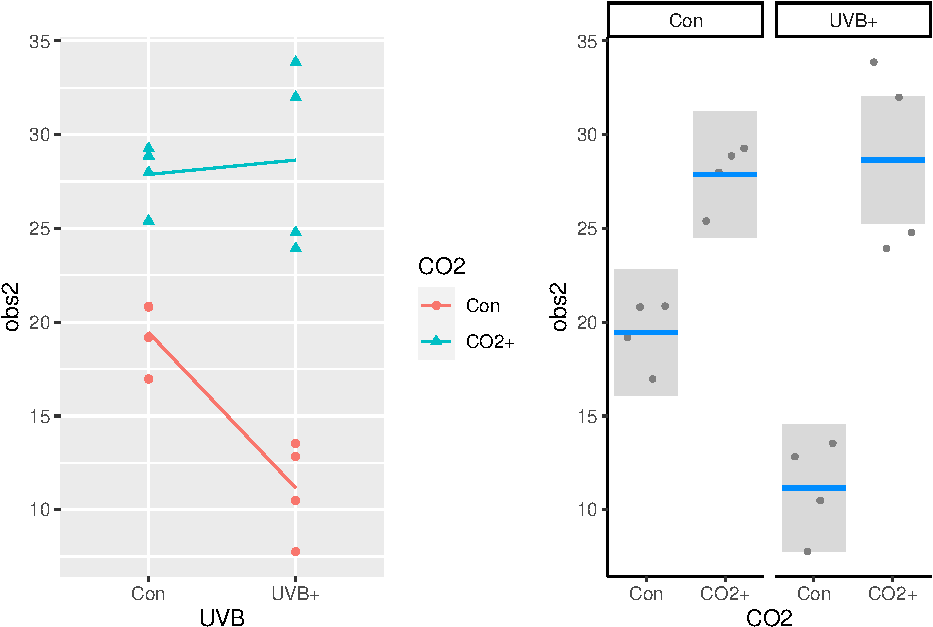
\includegraphics{Introduction-to-Experimental-Design-and-Analysis_files/figure-latex/unnamed-chunk-44-1.pdf}

\hypertarget{experimental-design-and-anova---a-summary}{%
\chapter{Experimental Design and ANOVA - A Summary}\label{experimental-design-and-anova---a-summary}}

There are three sets of things you should now know about based on reading these chapters and working through the examples. The first set is a bunch of clever R stuff for helping generate experimental designs. The second set is a better understanding of experimental designs in general. The third set is how to analyse and interpret data from 1-way and 2-way ANOVA models, that are the toolboxes for analysing these designs.

Lets review these in reverse order

\hypertarget{how-to-analyse-anova-models}{%
\section{How To Analyse ANOVA models}\label{how-to-analyse-anova-models}}

In semester 1, you were introduced to the 1-way ANOVA model, using the daphnia parasite data. Here you've learned more about those analyses.

You now understand better what treatment contrasts are, the risk of post-hoc tests like the Tukey Test, and methods for making \emph{a priori} contrasts to test specific hypothesis. You learned how specify specific hypoptheses and use the \texttt{fit.contrast} function from the \emph{gmodels} package to help you be really precise in asking and answering questions.

You also learned how to include a blocking factor in your models to control for environmental gradients in your experiments. You learned how to estimate the standard error that is used for the testing of among treatment level differences too.

Finally, you learned about the idea of interactions - the effect of UVB on Plant Yield Varies by CO2 level. You learned how to fit these models (e.g.~\texttt{lm(Yield\ \textasciitilde{}\ UVB\ *\ CO2,\ data\ =\ dataframe)}) and how to interpret the statistical outputs against the graphs you made. Speaking of which, you learned how tomake graphs that reveal the presence of interactions, or not.

\hypertarget{experimental-designs.}{%
\section{Experimental Designs.}\label{experimental-designs.}}

You should now understand the differences between, and value of the Completely Randomised Design, the Randomised Complete Block Design and the Latin Square Design. There are plenty more designs out there to manage lots of different issues. The \emph{agricolae} package is a great tool for generating designs (to help plan experminents) and is also a great resource for learning about them.

\url{https://myaseen208.github.io/agricolae/articles/Intro_agricolae.html}

\hypertarget{clever-r-stuff}{%
\section{Clever R Stuff}\label{clever-r-stuff}}

You've also increased your R ninja skills. You've learned about building `fake data' using the \texttt{design\_} class of functions in \emph{agricolae} mixed with random numbers and a clear set of tools that develop understanding of how additive and interactive effects arise among treatments in your data. This is a super skill.

There is nothing better than making data that has a pattern or not, to understand better where patterns are in your own data. If you can build `fake data' with and without the pattern you might expect from theory, then you have the template on which to examine carefully your `real data' collected via the experiments or surveys.

\hypertarget{introducing-the-ancova---the-analysis-of-covariance}{%
\chapter{Introducing the ANCOVA - the analysis of covariance}\label{introducing-the-ancova---the-analysis-of-covariance}}

In the previous chapters, we introduced classic experimental design principles, and in doing so, we focused on revisiting the 1-way ANOVA and introduced the 2-way ANOVA. In these models, the explanatory variables are categorical (they are factors). This means explanatory variable has distinct, discrete categories or \emph{levels}.

In many of our experiments, however, we might combine these categorical variables with a continuous variable. For example, we might estimate eggs produced as a function of body size and season or we might estimate the effect on plant growth rates of soil moisture in high versus low Nitrogen (N) conditions.

These simple examples describe an ANCOVA, where the one explanatory variable is continuous (e.g.~body size or soil moisture) and the other is categorical (e.g.~season or N-level). When this is the case, we are essentially combining the ANOVA with the Regression. If we recall that regression is largely about estimatinge slopes and intercepts, we might think, hey, COOL, so in an ANCOVA, we can ask if the categorical variable alters the slope or not\ldots..

What's very important to understand is that our core statement about interactions does not change.

\begin{quote}
The effect of X on Y varies by Z, translates to a) The effect of body size on egg production varies by season; or b) the effect of soil moisture on growth rate varies by N-level
\end{quote}

When written like this, the previous statements about slopes should be even more clear. The effect of body size (continuous) on egg production is a regression and we estimate a slope. We then can ask whether this slope is different between seasons.

\hypertarget{setting-up-the-various-ideas.}{%
\section{Setting up the various ideas.}\label{setting-up-the-various-ideas.}}

Let's start by looking at an example where the effect of Height on Weight varies by Sex. This is a classic set of data from numerous organisms\ldots. it captures biologically the question about sexual dimorphism - does the relationship between Height and Weight (a regression) vary by Sex (ANOVA)?

This relationship can take on many patterns.

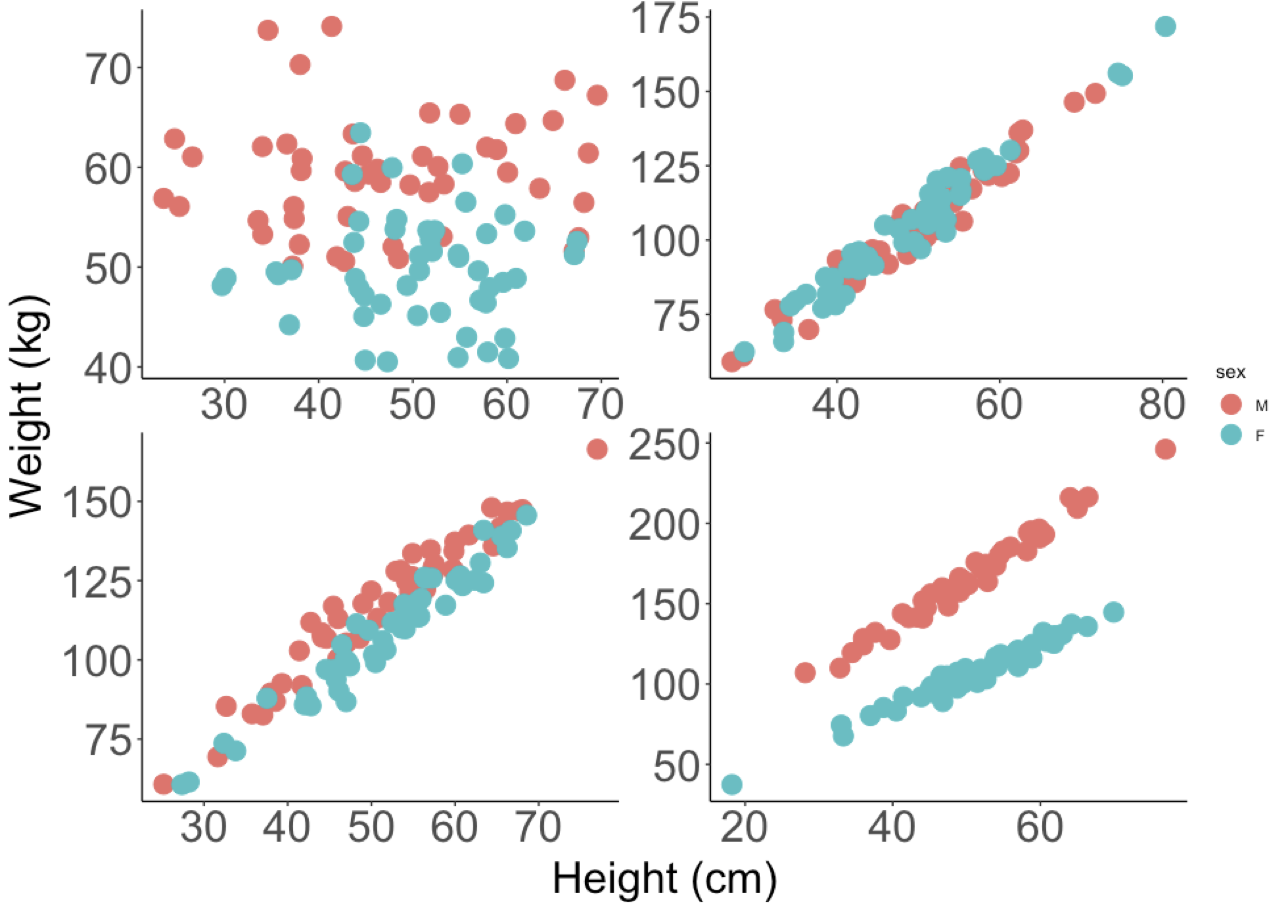
\includegraphics[width=17.89in]{images/ANCOVA_1}

\begin{itemize}
\tightlist
\item
  In the upper left we see a pattern where Males are heavier than Females, but there is no effect of Height on Weight.
\item
  In the upper right, we see that there is a positive relationship between Weight and Height, but no differences between Males and Females.
\item
  In the lower left, we might argue that there is a positive relationship between Weight and Height, that the relationship between Weight and Height does not vary (the slope is the same) and that Males are heavier (the red dots are mostly above the blue)
\item
  In the lower right, we see evidence of an interaction - the effect of Height on Weight (the slopes), varies by Sex.
\end{itemize}

It's quite important to recognise that each of patterns is possible outcome to testing the SAMEa hypothesis. The key thing to remember is that we have an a priori (in advance hypothesis). Regardless of the pattern, we should specify the appropriate model to test your the hypothesis and answer the question that motivated the design of the experiment and data collection.

For example, in these data, we fundamentally start with the question - does the effect of Height on Weight vary by Sex. The data might look like any of the above patterns. But as we started with that, we have to try and answer that question. And there is only one model syntax in the above figure that does this: \texttt{Weight\ \textasciitilde{}\ Height\ *\ Sex}. We'll expand on what this means as we work through the example.

\hypertarget{working-through-and-example.}{%
\section{Working through and example.}\label{working-through-and-example.}}

Let's work with a built in dataset in R - the Davis Study, which is exactly these data. The associated assignment is another example.

The process of doing this will follow a tried and true approach to analysing data. You should embed this workflow in your head:

\begin{enumerate}
\def\labelenumi{\arabic{enumi})}
\tightlist
\item
  PLOT the Data
\item
  Build the model to test the hypothesis
\item
  Check the Assumptions
\item
  Make Inference
\item
  Update the Figure for Publication
\end{enumerate}

\hypertarget{get-the-data-and-make-your-picture}{%
\subsection{Get the data and make your picture}\label{get-the-data-and-make-your-picture}}

The data are built into R, but embedded in the \texttt{carData} package, which was installed with the \texttt{car} package.

\begin{Shaded}
\begin{Highlighting}[]
\NormalTok{Davis }\OtherTok{\textless{}{-}}\NormalTok{ carData}\SpecialCharTok{::}\NormalTok{Davis}

\FunctionTok{glimpse}\NormalTok{(Davis)}
\end{Highlighting}
\end{Shaded}

\begin{verbatim}
## Rows: 200
## Columns: 5
## $ sex    <fct> M, F, F, M, F, M, M, M, M, M, M, F, F, F, F, F, M, F, M, F, ...
## $ weight <int> 77, 58, 53, 68, 59, 76, 76, 69, 71, 65, 70, 166, 51, 64, 52,...
## $ height <int> 182, 161, 161, 177, 157, 170, 167, 186, 178, 171, 175, 57, 1...
## $ repwt  <int> 77, 51, 54, 70, 59, 76, 77, 73, 71, 64, 75, 56, 52, 64, 57, ...
## $ repht  <int> 180, 159, 158, 175, 155, 165, 165, 180, 175, 170, 174, 163, ...
\end{verbatim}

\begin{Shaded}
\begin{Highlighting}[]
\FunctionTok{ggplot}\NormalTok{(Davis, }\FunctionTok{aes}\NormalTok{(}\AttributeTok{x =}\NormalTok{ height, }\AttributeTok{y =}\NormalTok{ weight, }\AttributeTok{col =}\NormalTok{ sex))}\SpecialCharTok{+}
  \FunctionTok{geom\_point}\NormalTok{()}
\end{Highlighting}
\end{Shaded}

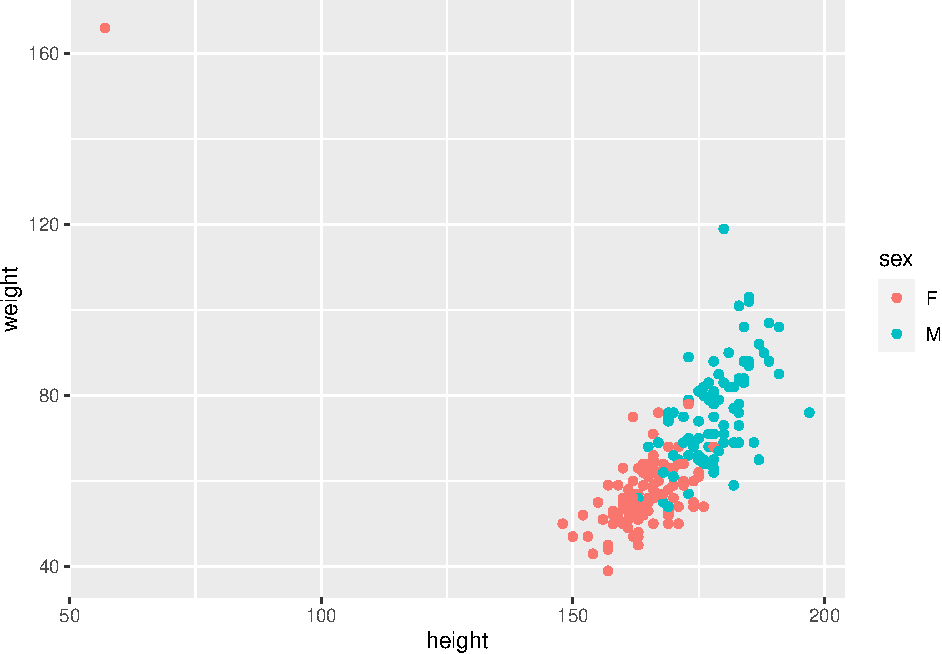
\includegraphics{Introduction-to-Experimental-Design-and-Analysis_files/figure-latex/unnamed-chunk-48-1.pdf}

Ahh\ldots. first hurdle\ldots. what's going on here? Well, always plot your data is totally justified, because it looks like one of the data points has the Height and Weight data entered incorrectly.

Let's fix that. Lets find the row, and make the change

\begin{Shaded}
\begin{Highlighting}[]
\CommentTok{\#which row? 12}
\NormalTok{Davis }\SpecialCharTok{\%\textgreater{}\%} \FunctionTok{filter}\NormalTok{(height }\SpecialCharTok{\textless{}} \DecValTok{100}\NormalTok{)}
\end{Highlighting}
\end{Shaded}

\begin{verbatim}
##    sex weight height repwt repht
## 12   F    166     57    56   163
\end{verbatim}

\begin{Shaded}
\begin{Highlighting}[]
\CommentTok{\# BASE R syntax to see each observation}
\NormalTok{Davis}\SpecialCharTok{$}\NormalTok{weight[}\DecValTok{12}\NormalTok{]}
\end{Highlighting}
\end{Shaded}

\begin{verbatim}
## [1] 166
\end{verbatim}

\begin{Shaded}
\begin{Highlighting}[]
\NormalTok{Davis}\SpecialCharTok{$}\NormalTok{height[}\DecValTok{12}\NormalTok{]}
\end{Highlighting}
\end{Shaded}

\begin{verbatim}
## [1] 57
\end{verbatim}

\begin{Shaded}
\begin{Highlighting}[]
\CommentTok{\# BASE R syntax to change them}
\NormalTok{Davis}\SpecialCharTok{$}\NormalTok{weight[}\DecValTok{12}\NormalTok{] }\OtherTok{\textless{}{-}} \DecValTok{57}
\NormalTok{Davis}\SpecialCharTok{$}\NormalTok{height[}\DecValTok{12}\NormalTok{] }\OtherTok{\textless{}{-}} \DecValTok{166}

\CommentTok{\# replot}
\FunctionTok{ggplot}\NormalTok{(Davis, }\FunctionTok{aes}\NormalTok{(}\AttributeTok{x =}\NormalTok{ height, }\AttributeTok{y =}\NormalTok{ weight, }\AttributeTok{col =}\NormalTok{ sex))}\SpecialCharTok{+}
  \FunctionTok{geom\_point}\NormalTok{()}
\end{Highlighting}
\end{Shaded}

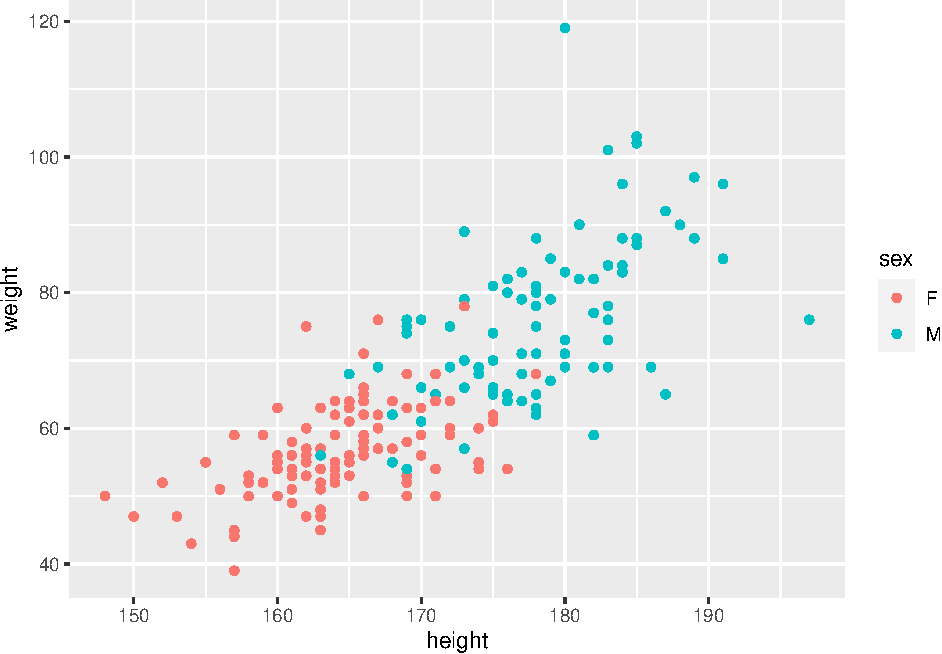
\includegraphics{Introduction-to-Experimental-Design-and-Analysis_files/figure-latex/unnamed-chunk-49-1.pdf}

Excellent. Lets look at this picture and ask ourselves whether the effect of Height on Weight appears to vary by Sex? What do you think?

We can actually get a bit of help here. We can use some ggplot magic to help us make this GUESS.
\textgreater{} NOTE: this is not doing statistics. This is using graphics to help guide our expectation of the outcome of doing the statistical test of our hypothesis.

\begin{Shaded}
\begin{Highlighting}[]
\FunctionTok{ggplot}\NormalTok{(Davis, }\FunctionTok{aes}\NormalTok{(}\AttributeTok{x =}\NormalTok{ height, }\AttributeTok{y =}\NormalTok{ weight, }\AttributeTok{col =}\NormalTok{ sex))}\SpecialCharTok{+}
  \FunctionTok{geom\_point}\NormalTok{()}\SpecialCharTok{+}
  \CommentTok{\# add a best fit line to each group (the sex category)}
  \FunctionTok{geom\_smooth}\NormalTok{(}\AttributeTok{method =}\NormalTok{ lm, }\AttributeTok{se =} \ConstantTok{FALSE}\NormalTok{)}
\end{Highlighting}
\end{Shaded}

\begin{verbatim}
## `geom_smooth()` using formula 'y ~ x'
\end{verbatim}

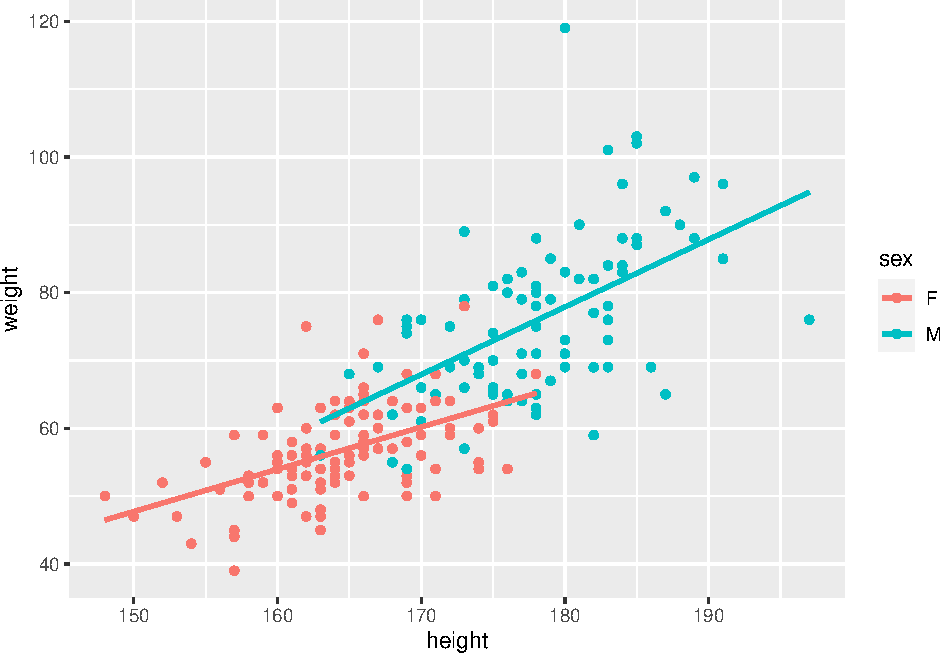
\includegraphics{Introduction-to-Experimental-Design-and-Analysis_files/figure-latex/unnamed-chunk-50-1.pdf}

Again, we have not `proven' anything or tested our hypothesis. What we have is a good guess though. We can guess that

\begin{enumerate}
\def\labelenumi{\arabic{enumi}.}
\tightlist
\item
  Males are heavier than females (what is the difference in the intercepts?)
\item
  The effect of height on weight is positive (the slope(s) are positive, not negative)
\item
  There might be a difference in slopes - the Male line is steeper.
\end{enumerate}

We might even go as far to estimate by eye the slope assuming that there is no effect of Sex. Recalling that the slope is the rise/run or the change in y over the change in x, we can guess that the slope is \textasciitilde{} (100-40)/(200-140) = (60/60) = 1. We are not expecting much variation around that. But if we see the statistics returning a value 10x more or less than this, we should be concerned!

\hypertarget{building-the-model-and-understanding-it}{%
\section{Building the model (and understanding it)}\label{building-the-model-and-understanding-it}}

The next step is to build the model to test our hypothesis. As we declared above, the model to test the interaction is \texttt{lm(weight\ \textasciitilde{}\ height\ *\ sex,\ data\ =\ Davis)}. Let's discuss this a bit.

First, this model expands to the following full description:

\texttt{lm(weight\ \textasciitilde{}\ height\ +\ sex\ +\ height:sex,\ data\ =\ Davis)}

This reads as "Weight is a function of the effect of Height (slope), Sex (intercept) and the interaction between Height and Sex (do the slopes vary?). The \texttt{Height\ *\ Sex} syntax always expands to this \emph{full model} - the model containing the main effects and the interaction.

OK. Let's fit the model

\begin{Shaded}
\begin{Highlighting}[]
\CommentTok{\# we call the model mod\_Davis.}
\NormalTok{mod\_Davis }\OtherTok{\textless{}{-}} \FunctionTok{lm}\NormalTok{(weight }\SpecialCharTok{\textasciitilde{}}\NormalTok{ height }\SpecialCharTok{+}\NormalTok{ sex }\SpecialCharTok{+}\NormalTok{ height}\SpecialCharTok{:}\NormalTok{sex, }\AttributeTok{data =}\NormalTok{ Davis)}
\end{Highlighting}
\end{Shaded}

That's it. We've got the model. But before we make any attempts at actually evaluating our test of the hypothesis, we have to check the assumptions!

To do this, we use the autplot function from the ggfortify package.

\begin{Shaded}
\begin{Highlighting}[]
\FunctionTok{autoplot}\NormalTok{(mod\_Davis)}
\end{Highlighting}
\end{Shaded}

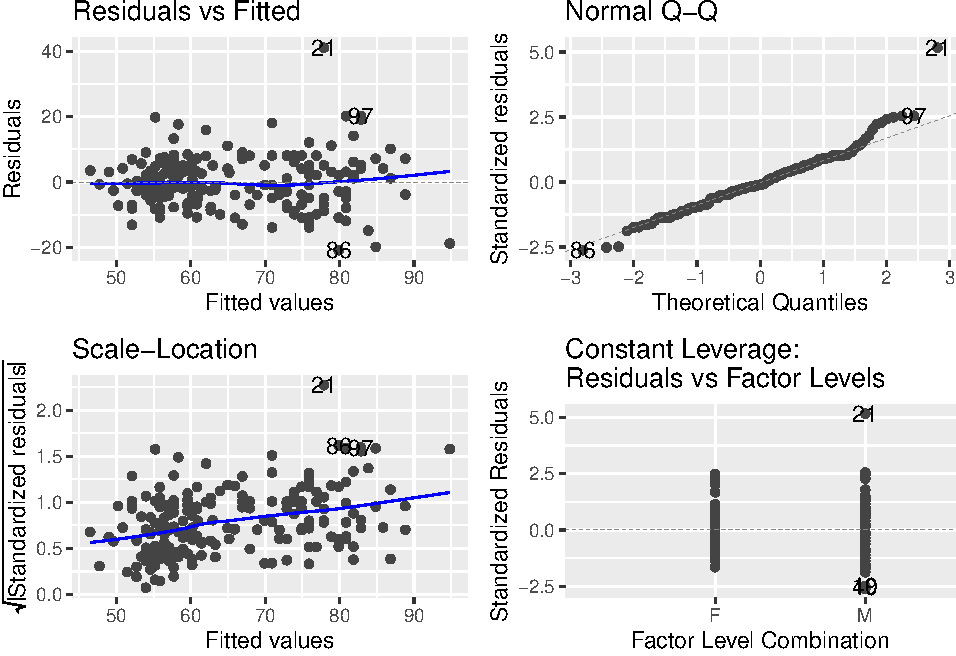
\includegraphics{Introduction-to-Experimental-Design-and-Analysis_files/figure-latex/unnamed-chunk-52-1.pdf}

OK. Let's walk through the three core diagnostics.

In the upper left, we are evaluating the systematic part of the model - are there any systematic departures from the linear model we've speficied? Are there interactions missing or specific nonlinearities? Nope.

In the upper right, we are evaluating the normality of the residuals. These too look pretty good.

In the lower left, we are evalauting the assumption of a constant mean-variance relationship. Oops.

\hypertarget{dealing-with-some-issues-with-residuals.}{%
\subsection{Dealing with some issues with residuals.}\label{dealing-with-some-issues-with-residuals.}}

The above issue is one we can deal with via a \emph{transformation}. Let's start with the facts\ldots. When the variance increases with the mean, one transformation that can work is the logarithm of the continuous variables.

ADD DYLANS STUFF FROM MEE PAPERS and Mean - VARIANCE

\begin{Shaded}
\begin{Highlighting}[]
\CommentTok{\# re{-}plot with log{-}log}
\FunctionTok{ggplot}\NormalTok{(}\AttributeTok{data =}\NormalTok{ Davis, }\FunctionTok{aes}\NormalTok{(}\AttributeTok{x =} \FunctionTok{log}\NormalTok{(height), }\AttributeTok{y =} \FunctionTok{log}\NormalTok{(weight), }\AttributeTok{col =}\NormalTok{ sex))}\SpecialCharTok{+}
  \FunctionTok{geom\_point}\NormalTok{()}\SpecialCharTok{+}
  \FunctionTok{geom\_smooth}\NormalTok{(}\AttributeTok{method =}\NormalTok{ lm, }\AttributeTok{se =} \ConstantTok{FALSE}\NormalTok{)}
\end{Highlighting}
\end{Shaded}

\begin{verbatim}
## `geom_smooth()` using formula 'y ~ x'
\end{verbatim}

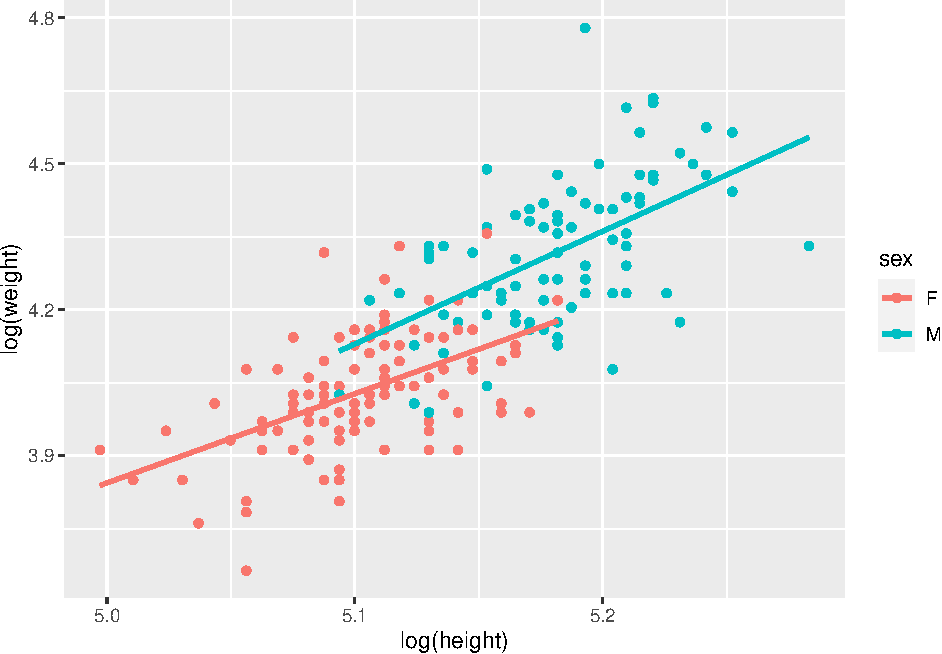
\includegraphics{Introduction-to-Experimental-Design-and-Analysis_files/figure-latex/unnamed-chunk-53-1.pdf}

\begin{Shaded}
\begin{Highlighting}[]
\CommentTok{\# fit the model {-} note we can specify the transformation RIGHT IN THE MODEL}
\NormalTok{mod\_Davis\_log }\OtherTok{\textless{}{-}} \FunctionTok{lm}\NormalTok{(}\FunctionTok{log}\NormalTok{(weight) }\SpecialCharTok{\textasciitilde{}} \FunctionTok{log}\NormalTok{(height) }\SpecialCharTok{*}\NormalTok{ sex, }\AttributeTok{data =}\NormalTok{ Davis)}

\CommentTok{\# check the new residuals}
\FunctionTok{autoplot}\NormalTok{(mod\_Davis\_log)}
\end{Highlighting}
\end{Shaded}

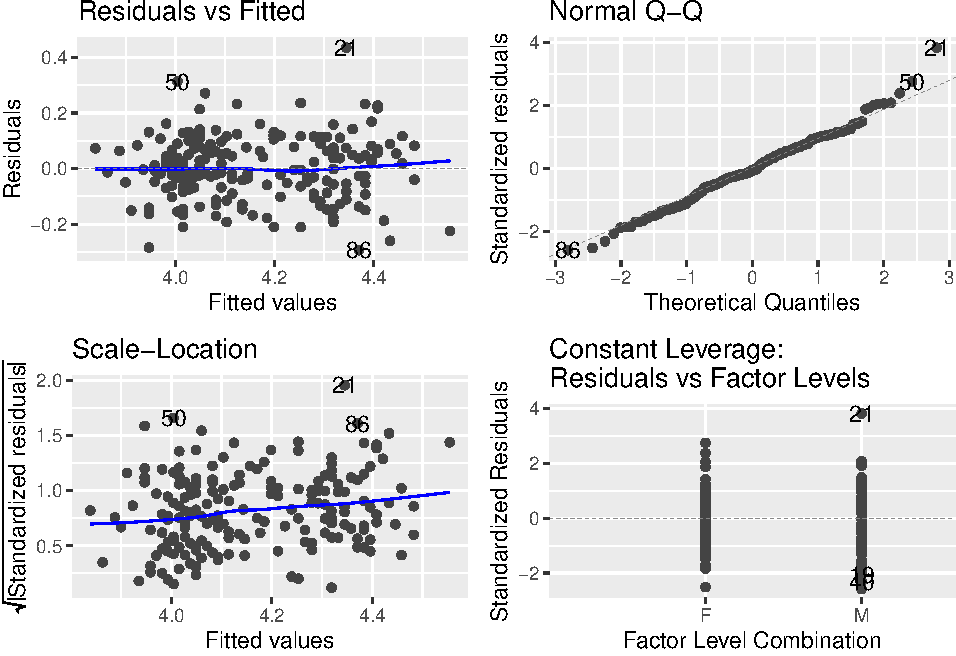
\includegraphics{Introduction-to-Experimental-Design-and-Analysis_files/figure-latex/unnamed-chunk-53-2.pdf}

This is definitely flatter - you can tell by the range on the y-axis of the scale-location plot.

So, we can now move to evaluating the model. You are probably thinking about what it means to analyse the data on the log-log axis\ldots. we will come to that shortly.

\hypertarget{making-inference-on-the-ancova}{%
\subsection{Making inference on the ANCOVA}\label{making-inference-on-the-ancova}}

OK. So, the next step is to use review the ANOVA table - yes, we use the same Anova function to build an anova table to explore the results of an ANCOVA.

Let's revisit our initial guesses and work through what the model is telling us:

\begin{enumerate}
\def\labelenumi{\arabic{enumi}.}
\tightlist
\item
  Males are heavier than females (what is the difference in the intercepts?)
\item
  The effect of height on weight is positive (the slope(s) are positive, not negative)
\item
  There might be a difference in slopes - the Male line is steeper.
  `
\end{enumerate}

\begin{Shaded}
\begin{Highlighting}[]
\FunctionTok{anova}\NormalTok{(mod\_Davis\_log)}
\end{Highlighting}
\end{Shaded}

\begin{verbatim}
## Analysis of Variance Table
## 
## Response: log(weight)
##                  Df Sum Sq Mean Sq  F value    Pr(>F)    
## log(height)       1 4.6643  4.6643 357.4735 < 2.2e-16 ***
## sex               1 0.3446  0.3446  26.4115 6.647e-07 ***
## log(height):sex   1 0.0144  0.0144   1.1038    0.2947    
## Residuals       196 2.5574  0.0130                       
## ---
## Signif. codes:  0 '***' 0.001 '**' 0.01 '*' 0.05 '.' 0.1 ' ' 1
\end{verbatim}

The table tells us that there is no evidence for an interaction. The last line of this table contains the p-value for the interaction. It is testing the null hypothesis that the slopes are the same. We can not reject this null hypothesis. There is no evidence that allowing the slopes for Males and Females be different is supported. That's the answer to guess 3 above. It is also the answer to our question: does the effect of Height on Weight vary by Sex. Nope.

However, we do detect \emph{main effects} of height and sex. This means that each of these DOES have an effect - but we say the effects are additive.

Great. What this means is that the data actually conform to picture in the lower left.

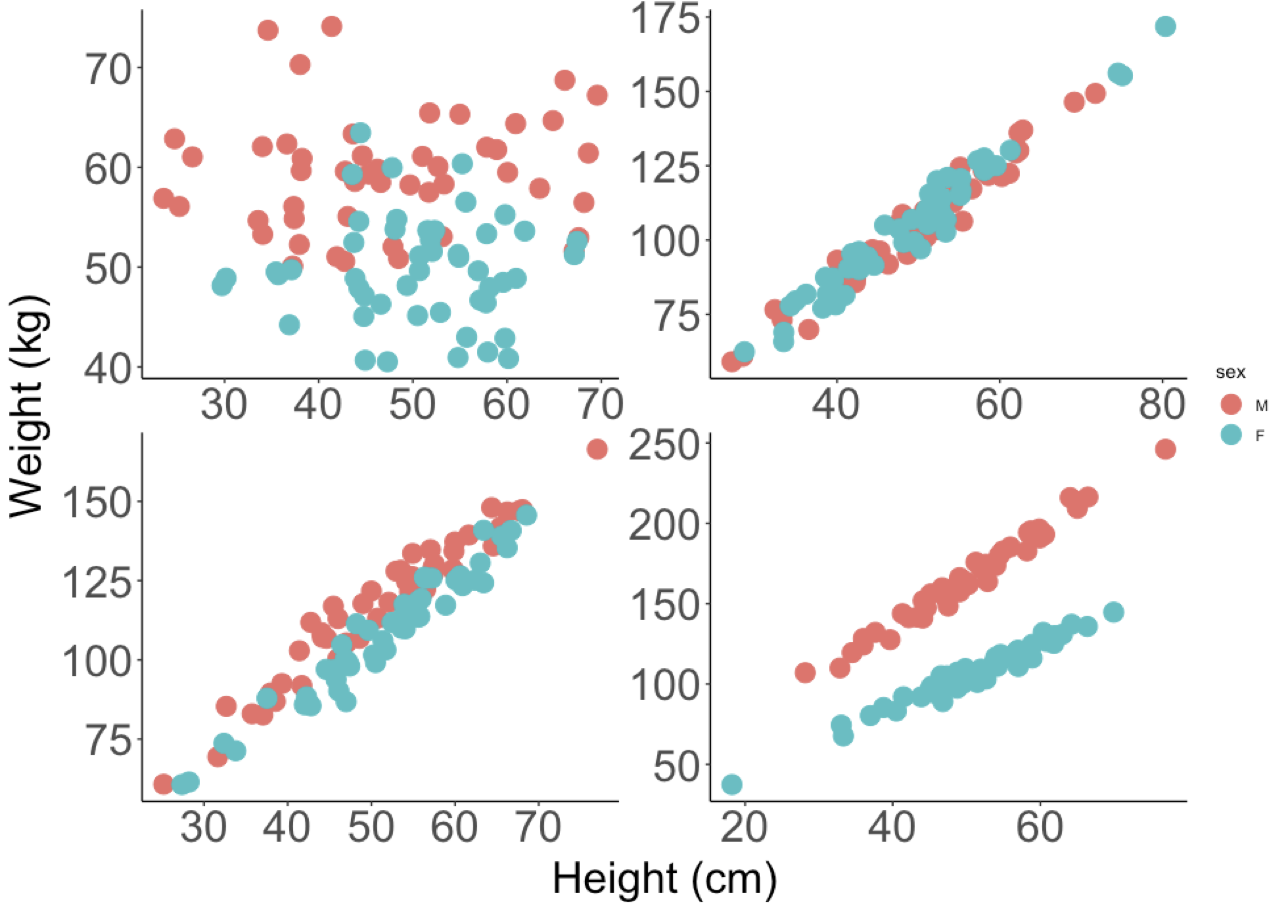
\includegraphics[width=17.89in]{images/ANCOVA_1}

There is a slope associated with Height (we don't know whether it's positive or not, but we think it is), and there is an effect of sex (we don't know whether Males are heavier yet). What we can say, with confidence, is this.

\begin{quote}
The effect of height on weight did not vary by sex (F = 1.01, df = 1,196, p = 0.29). The effect of sex (F, df, p) and height (F, df, p) are thus additive on Weight.
\end{quote}

Another way to read this is the following:

When we allow for a common slope associated with logHeight, we capture 4.66 units of variation in weight, which when compared to the 0.013 units of variation left over (residual MSE), is alot. The F is thus BIG and the p-value small. When we allow for an effect of Sex to define different average weights, this too is important as it captures 0.344 units of variation in weight, which comparied to the 0.013 units in the residual, is also big (Big F, small P). However, when we allow for the slopes caused by height to vary with sex, this captures very little variation with respect to the residual variation (0.014 comprared to 0.013) hence a small F and a large P.

\hypertarget{the-summary-table-and-making-sense-of-the-log-stuff.}{%
\subsection{The summary table and making sense of the log stuff.}\label{the-summary-table-and-making-sense-of-the-log-stuff.}}

Let's start investigating the actual details via the \texttt{summary} table:

\begin{Shaded}
\begin{Highlighting}[]
\FunctionTok{summary}\NormalTok{(mod\_Davis\_log)}
\end{Highlighting}
\end{Shaded}

\begin{verbatim}
## 
## Call:
## lm(formula = log(weight) ~ log(height) * sex, data = Davis)
## 
## Residuals:
##      Min       1Q   Median       3Q      Max 
## -0.29310 -0.06543 -0.00592  0.07420  0.43410 
## 
## Coefficients:
##                  Estimate Std. Error t value Pr(>|t|)    
## (Intercept)       -5.3202     1.6016  -3.322  0.00107 ** 
## log(height)        1.8329     0.3138   5.841 2.13e-08 ***
## sexM              -2.3724     2.3765  -0.998  0.31936    
## log(height):sexM   0.4852     0.4618   1.051  0.29473    
## ---
## Signif. codes:  0 '***' 0.001 '**' 0.01 '*' 0.05 '.' 0.1 ' ' 1
## 
## Residual standard error: 0.1142 on 196 degrees of freedom
## Multiple R-squared:  0.6626, Adjusted R-squared:  0.6575 
## F-statistic: 128.3 on 3 and 196 DF,  p-value: < 2.2e-16
\end{verbatim}

This table reports on the \emph{treatment contrasts} we introduced earlier this semester. Let's walk through the details.

The first two rows correspond to one of the sexes. Can you identify which one? The hint is looking at the other rows. They have an M after them. M comes after F. So the first two rows correspond to the intercept and slope of the Females.

You may be asking why the intercept is a negative number. A simple look back at the range of the x-axis should answer this\ldots{} the y intercept occurs at x = 0, right?

You should understand, from the principles of an equation for a line, the following:

\begin{quote}
the effect of height on weight for females is \texttt{log(weightF)\ =\ -5.31\ +\ 1.82*log(heightF)}.
\end{quote}

OK\ldots{} let's interpret what the next two lines mean. The third line is labelled \texttt{SexM.} The fourth is labelled \texttt{logHeight:SexM}. Any guesses as to which is associated with the slope and which the intercept?

One trick, again, is to recognise the syntax -\textgreater{} the presence of the \texttt{:} is indicative of the interaction which is the thing that lets slopes vary. So, \texttt{SexM} is about intercepts and \texttt{logHeight:SexM} is about slopes. But what are they?

Please recall from previous work that treatment contrasts are about DIFFERENCES. Thus, the \texttt{sexM} term is a difference between the female and make intercept and the \texttt{logHeight:SexM} is about the difference between the female and make slopes.

This allows the following maths\ldots.

\texttt{log(weightF)\ =\ -5.31\ +\ 1.82*log(heightF)}

\texttt{log(weightM)\ =\ (-5.31-2.37)\ +\ (1.82+0.48)*(log(heightF))}

However, we know that the 0.48 increase in the slope is not siginficant, and as a result, the -2.37 increase in the intercept is also not correct.

\hypertarget{the-equations-supported-by-the-model.}{%
\subsection{The equations supported by the model.}\label{the-equations-supported-by-the-model.}}

In order to identify the equations supported by the model, we can refit the model to reflect the ADDITIVE effects only.

\begin{Shaded}
\begin{Highlighting}[]
\NormalTok{mod\_Davis\_log2 }\OtherTok{\textless{}{-}} \FunctionTok{lm}\NormalTok{(}\FunctionTok{log}\NormalTok{(weight) }\SpecialCharTok{\textasciitilde{}} \FunctionTok{log}\NormalTok{(height) }\SpecialCharTok{+}\NormalTok{ sex, }\AttributeTok{data =}\NormalTok{ Davis)}
\FunctionTok{summary}\NormalTok{(mod\_Davis\_log2)}
\end{Highlighting}
\end{Shaded}

\begin{verbatim}
## 
## Call:
## lm(formula = log(weight) ~ log(height) + sex, data = Davis)
## 
## Residuals:
##      Min       1Q   Median       3Q      Max 
## -0.28714 -0.06906 -0.00978  0.07615  0.43717 
## 
## Coefficients:
##             Estimate Std. Error t value Pr(>|t|)    
## (Intercept) -6.46349    1.17541  -5.499 1.18e-07 ***
## log(height)  2.05688    0.23030   8.931 2.99e-16 ***
## sexM         0.12417    0.02417   5.138 6.66e-07 ***
## ---
## Signif. codes:  0 '***' 0.001 '**' 0.01 '*' 0.05 '.' 0.1 ' ' 1
## 
## Residual standard error: 0.1143 on 197 degrees of freedom
## Multiple R-squared:  0.6607, Adjusted R-squared:  0.6573 
## F-statistic: 191.8 on 2 and 197 DF,  p-value: < 2.2e-16
\end{verbatim}

Right, now we get our expected pattern:

\texttt{log(weightF)\ =\ -6.46\ +\ 2.05*log(heightF)}

\texttt{log(weightM)\ =\ (-6.46\ +\ 0.12)\ +\ 2.05*log(heightF)}

We can see the common slope and the slightly higher average weight (0.12 units!) of males.

\hypertarget{making-even-more-inference-and-drawing-the-picture}{%
\subsection{Making even more inference and drawing the picture}\label{making-even-more-inference-and-drawing-the-picture}}

OK, lets use some plotting tricks and get a nice picture:

\begin{Shaded}
\begin{Highlighting}[]
\CommentTok{\# first create a data frame to use that combines the raw data }
\CommentTok{\# with the predictions from the model}
\CommentTok{\# note that the model is the ADDITIVE model, for plotting}
\NormalTok{plotThis }\OtherTok{\textless{}{-}}\NormalTok{ Davis }\SpecialCharTok{\%\textgreater{}\%} 
  \FunctionTok{mutate}\NormalTok{(}\AttributeTok{preds =} \FunctionTok{predict}\NormalTok{(mod\_Davis\_log2))}

\CommentTok{\# now, make lines with the model predictions}
\CommentTok{\# and add the points as the raw data}
\CommentTok{\# pay attention to where we are using log()!}
\FunctionTok{ggplot}\NormalTok{(plotThis, }\FunctionTok{aes}\NormalTok{(}\AttributeTok{x =} \FunctionTok{log}\NormalTok{(height), }\AttributeTok{y =}\NormalTok{ preds, }\AttributeTok{col =}\NormalTok{ sex))}\SpecialCharTok{+}
  \FunctionTok{geom\_line}\NormalTok{()}\SpecialCharTok{+}
  \FunctionTok{geom\_point}\NormalTok{(}\FunctionTok{aes}\NormalTok{(}\AttributeTok{y =} \FunctionTok{log}\NormalTok{(weight)))}
\end{Highlighting}
\end{Shaded}

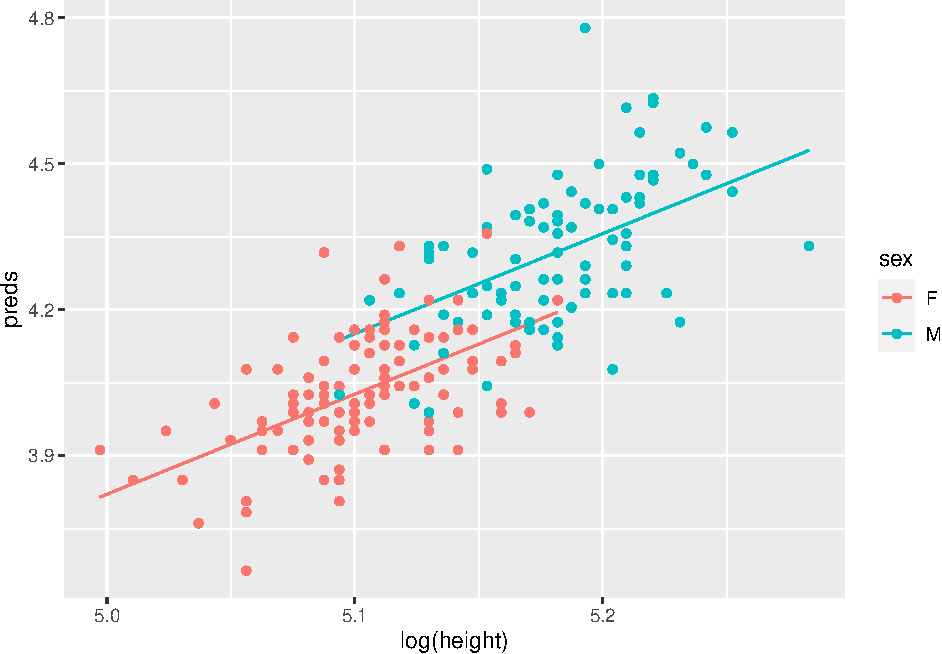
\includegraphics{Introduction-to-Experimental-Design-and-Analysis_files/figure-latex/unnamed-chunk-58-1.pdf}

Great. Now we can see that the full model (mod\_Davis\_log) told us. The lines are parallel. There is no interaction.

In fact, we can do a bit more here.

Remember that the model says

For women log(weight)= -6.46 + 2.05 * log(height)
For men log(weight)= (-6.46 + 0.12) + 2.05 * log(height)

Because we are in log land, we can do some clever maths: We know that

\texttt{log(weight\ Female)\ -\ log(weight\ Male)\ =\ -\ 0.12}

(this is the treatment contrast for the intercept). We also know (please memorise) that the difference between logs is equal to the log of the ratio:

\texttt{log(weightF/weightM)\ =\ -0.12}

Finally, we can convert both sides to non-log by exponentiating:

\texttt{exp(log(weightF/weightM))\ =\ exp(-0.12)\ =\ 0.88}

What does this mean? At any given height, female weight is 88\% of a makes (12\% lower).

Cool! That's one of the benefits of log-log linear relationships. The ratio of the categories in log-log land directly translates to a percent difference between the groups.

It's also worth noting that the height slope is \textasciitilde2, which suggests\ldots{} yes\ldots{} because we are in log-land, that weight scales with \(height^2\).

One way to `test' this is to ask whether estimating the log(weight) slope improve the fit of the model compared to fixing it at 2. Here are ways: `by hand' and by a function in the \texttt{car} package.

\begin{Shaded}
\begin{Highlighting}[]
\CommentTok{\# by hand}
\CommentTok{\# we use the offset function to fix the slope of height at 2}
\NormalTok{mod\_Davis\_offset }\OtherTok{\textless{}{-}}\FunctionTok{lm}\NormalTok{(}\FunctionTok{log}\NormalTok{(weight) }\SpecialCharTok{\textasciitilde{}}\NormalTok{  sex }\SpecialCharTok{+} \FunctionTok{offset}\NormalTok{(}\DecValTok{2}\SpecialCharTok{*}\FunctionTok{log}\NormalTok{(height)), }\AttributeTok{data=}\NormalTok{Davis)}

\CommentTok{\# then compare it to the model where we estimate it freely.}
\FunctionTok{anova}\NormalTok{(mod\_Davis\_log2, mod\_Davis\_offset)}
\end{Highlighting}
\end{Shaded}

\begin{verbatim}
## Analysis of Variance Table
## 
## Model 1: log(weight) ~ log(height) + sex
## Model 2: log(weight) ~ sex + offset(2 * log(height))
##   Res.Df    RSS Df  Sum of Sq     F Pr(>F)
## 1    197 2.5718                           
## 2    198 2.5726 -1 -0.0007962 0.061 0.8052
\end{verbatim}

\begin{Shaded}
\begin{Highlighting}[]
\CommentTok{\# by car package}
\NormalTok{car}\SpecialCharTok{::}\FunctionTok{linearHypothesis}\NormalTok{(mod\_Davis\_log2, }\StringTok{"log(height) = 2"}\NormalTok{) }\CommentTok{\# the estimate IS 2}
\end{Highlighting}
\end{Shaded}

\begin{verbatim}
## Linear hypothesis test
## 
## Hypothesis:
## log(height) = 2
## 
## Model 1: restricted model
## Model 2: log(weight) ~ log(height) + sex
## 
##   Res.Df    RSS Df Sum of Sq     F Pr(>F)
## 1    198 2.5726                          
## 2    197 2.5718  1 0.0007962 0.061 0.8052
\end{verbatim}

\begin{Shaded}
\begin{Highlighting}[]
\NormalTok{car}\SpecialCharTok{::}\FunctionTok{linearHypothesis}\NormalTok{(mod\_Davis\_log2, }\StringTok{"log(height) = 0"}\NormalTok{) }\CommentTok{\# the estimate IS NOT 0.}
\end{Highlighting}
\end{Shaded}

\begin{verbatim}
## Linear hypothesis test
## 
## Hypothesis:
## log(height) = 0
## 
## Model 1: restricted model
## Model 2: log(weight) ~ log(height) + sex
## 
##   Res.Df    RSS Df Sum of Sq      F   Pr(>F)    
## 1    198 3.6131                                 
## 2    197 2.5718  1    1.0413 79.768 2.99e-16 ***
## ---
## Signif. codes:  0 '***' 0.001 '**' 0.01 '*' 0.05 '.' 0.1 ' ' 1
\end{verbatim}

\hypertarget{some-general-principles}{%
\section{Some General Principles}\label{some-general-principles}}

\hypertarget{ancova-always-tests-the-interaction-against-the-additive-model}{%
\subsection{ANCOVA always tests the interaction against the additive model}\label{ancova-always-tests-the-interaction-against-the-additive-model}}

This figure highlights the various models and interpretations associated with the pieces of an ANCOVA dataset. This is a way to envision all of the potential linear relationships among the variables that might arise in an experiment with a continuous and categorical explanatory variable.

Note that just because your data looks like a particular pattern doesn't mean you should use that model. Your statistical model should be driven by your question and original design.

\begin{figure}
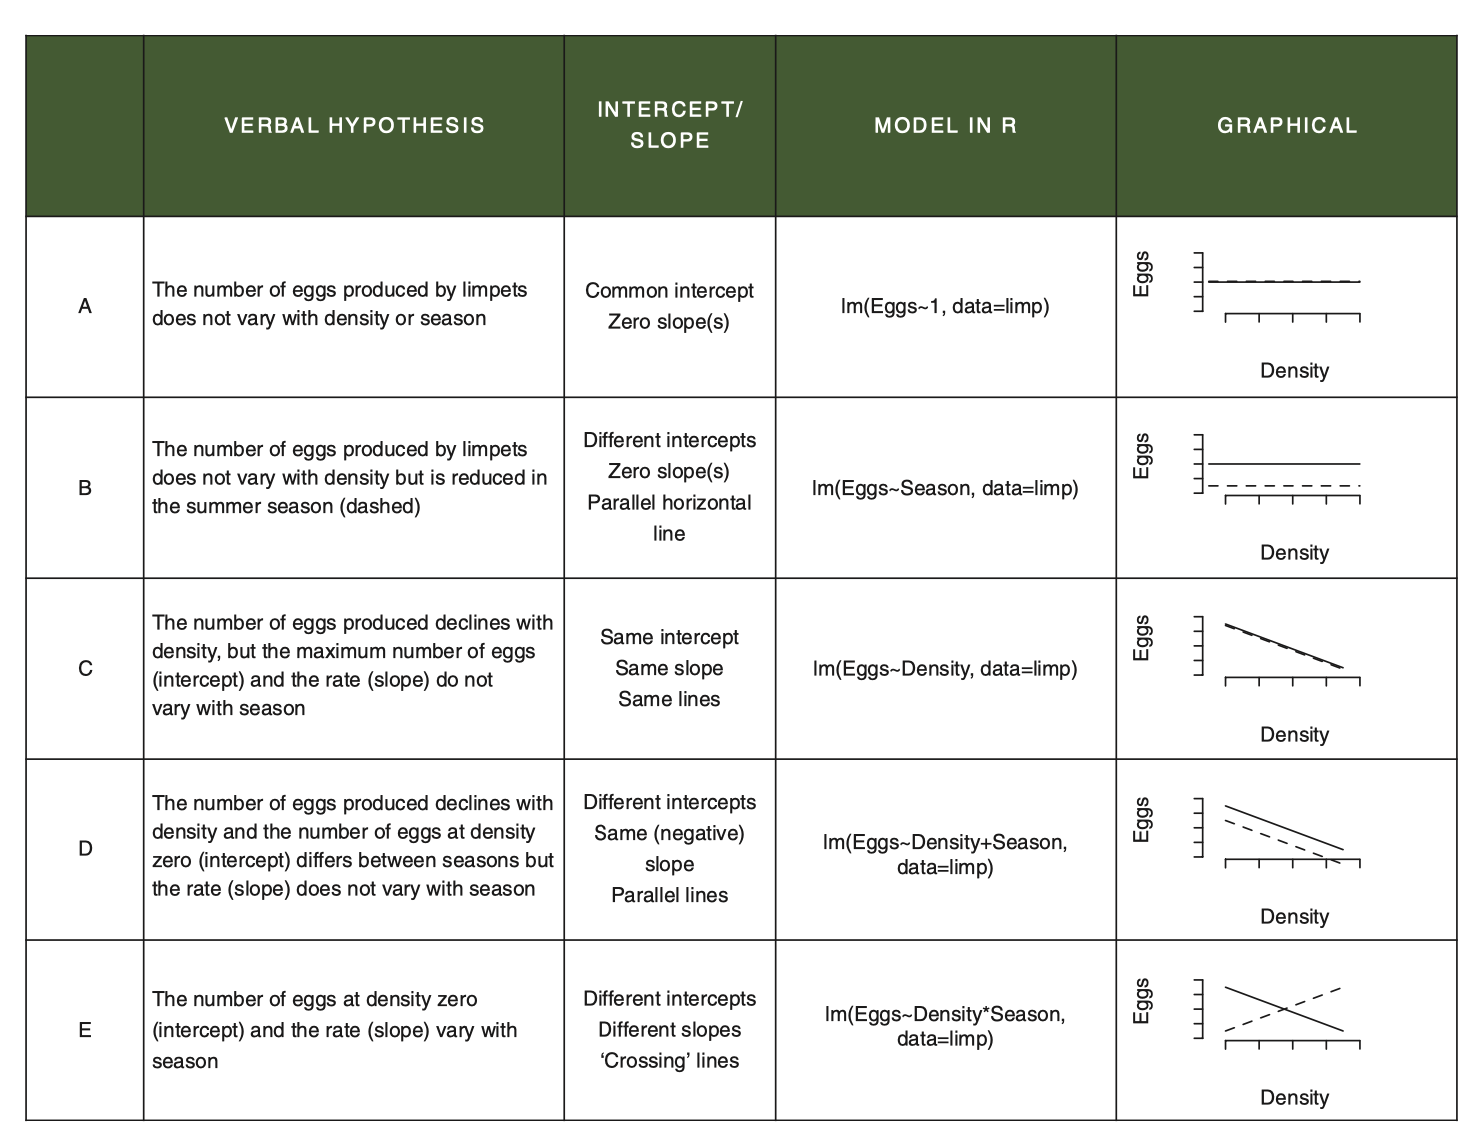
\includegraphics[width=20.56in]{images/GSwithR_Grid} \caption{From Getting Started with R, 2nd Edition, OUP}\label{fig:unnamed-chunk-60}
\end{figure}

For example, if you design a study with an ANCOVA question in mind, you are always starting your analysis with the question of whether the effect of X on Y varies by Z. Thus, ANCOVA always starts with comparing the interaction (model E) against the additive model (model D).

\begin{quote}
Proof: If we compare the additive model and the model with the interaction, we are specifically testing for whether allowing the slopes to vary by sex \emph{explains additional variation} above and beyond the main, additive effects of height and sex. To do this, we use \texttt{anova()} but pass it two models. This does what is called a Liklihood Ratio Test.
Compare the result of the first test to the last line of the second. This proves that when we fit model E, the test for the interaction is a comparison with model D!
\end{quote}

\begin{Shaded}
\begin{Highlighting}[]
\FunctionTok{anova}\NormalTok{(mod\_Davis\_log, mod\_Davis\_log2)}
\end{Highlighting}
\end{Shaded}

\begin{verbatim}
## Analysis of Variance Table
## 
## Model 1: log(weight) ~ log(height) * sex
## Model 2: log(weight) ~ log(height) + sex
##   Res.Df    RSS Df Sum of Sq      F Pr(>F)
## 1    196 2.5574                           
## 2    197 2.5718 -1 -0.014402 1.1038 0.2947
\end{verbatim}

\begin{Shaded}
\begin{Highlighting}[]
\FunctionTok{Anova}\NormalTok{(mod\_Davis\_log)}
\end{Highlighting}
\end{Shaded}

\begin{verbatim}
## Anova Table (Type II tests)
## 
## Response: log(weight)
##                  Sum Sq  Df F value    Pr(>F)    
## log(height)     1.04135   1 79.8099 3.024e-16 ***
## sex             0.34461   1 26.4115 6.647e-07 ***
## log(height):sex 0.01440   1  1.1038    0.2947    
## Residuals       2.55738 196                      
## ---
## Signif. codes:  0 '***' 0.001 '**' 0.01 '*' 0.05 '.' 0.1 ' ' 1
\end{verbatim}

\hypertarget{specifying-models-in-r}{%
\subsection{Specifying models in R}\label{specifying-models-in-r}}

We can add terms
\texttt{weight\ \textasciitilde{}\ sex\ +\ height}

Have crossed terms
\texttt{weight\ \textasciitilde{}\ sex\ *\ height} which is \texttt{weight\ \textasciitilde{}\ sex\ +\ \ height\ +\ sex\ :\ height}

Remove terms
\texttt{weight\ \textasciitilde{}\ sex\ *\ height\ –\ sex\ :\ height} which is \texttt{weight\textasciitilde{}\ sex\ +\ \ height}

Include all interactions up to order k
\texttt{weight\textasciitilde{}\ (sex\ +\ height\ +\ age)\^{}2} which is \texttt{sex\ +\ height\ +\ age\ +\ sex\ :\ height\ +\ sex\ :\ age\ +\ age\ :\ height}

\hypertarget{nonlinearities-polynomials-and-regression}{%
\chapter{Nonlinearities, polynomials and regression}\label{nonlinearities-polynomials-and-regression}}

If you recall from chapter 1, we introduced the general linear model, and finished with an example where the data were highly non-linear and based on the following equation

\(y = 0.01 + x^{2} + \epsilon\)

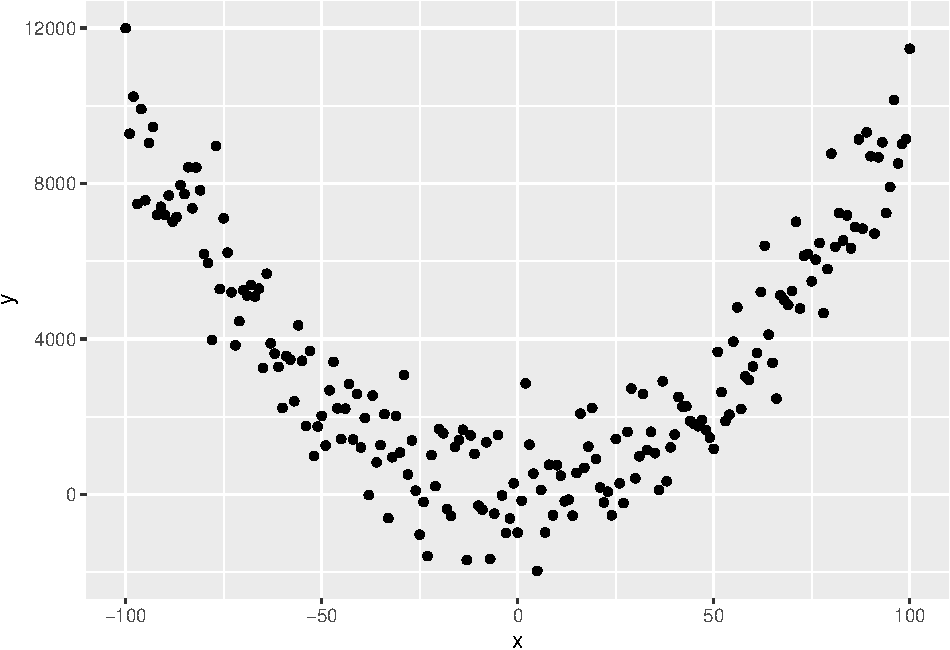
\includegraphics{Introduction-to-Experimental-Design-and-Analysis_files/figure-latex/unnamed-chunk-63-1.pdf}

In this final section of the module, we are going to analyse a nonlinear relationship using a linear model. This exercise should accomplish two tasks. First, it will show you how to build models to capture non-linearity. Second, it will reinforce how we use the diagnostic tools to critique our model before moving on to make inference.

\hypertarget{transformations---a-reminder-and-starting-point.}{%
\section{Transformations - a reminder and starting point.}\label{transformations---a-reminder-and-starting-point.}}

Transformations, as we discussed in previous chapters, allow lots of models to be expressed as a linear model.

For example the model for exponential growth (Numbers vs Time)

\(N_{t}=N_{0}*e^{(r*t)}\)

Remembering some rules of logrithms, this can be expressed as a linear model as:

\(log(N_{t})=log(N_{0}) + r*t\)

Here, \(log(N_{0})\) is the y-intercept and \(r\) is the gradient or slope, and \(t\) = time is the x-axis explanatory variable and \(log(N)\) is the y-axis response variable.

\hypertarget{working-through-an-example.}{%
\section{Working through an example.}\label{working-through-an-example.}}

Don't forget that you need the \texttt{tidyverse}, \texttt{car} and \texttt{ggfortify} packages (use \texttt{library()}) to make all of this work!

We are going to work with a built in dataset about cars to demonstrate how to detect and model non-linearities. This is an exercise in multiple regression and in using the diagnostic plots.

The data are built into R and we don't need to do anything but remember that the dataset is called cars. Lets see what it looks like. The \texttt{speed} is how fast the car is going before it is `asked' to stop, and the \texttt{dist} variable is how long it takes to stop in m

\begin{Shaded}
\begin{Highlighting}[]
\FunctionTok{glimpse}\NormalTok{(cars)}
\end{Highlighting}
\end{Shaded}

\begin{verbatim}
## Rows: 50
## Columns: 2
## $ speed <dbl> 4, 4, 7, 7, 8, 9, 10, 10, 10, 11, 11, 12, 12, 12, 12, 13, 13,...
## $ dist  <dbl> 2, 10, 4, 22, 16, 10, 18, 26, 34, 17, 28, 14, 20, 24, 28, 26,...
\end{verbatim}

Let's start with step 1: making a good picture.

\begin{Shaded}
\begin{Highlighting}[]
\FunctionTok{ggplot}\NormalTok{(cars, }\FunctionTok{aes}\NormalTok{(}\AttributeTok{x =}\NormalTok{ speed, }\AttributeTok{y =}\NormalTok{ dist))}\SpecialCharTok{+}
  \FunctionTok{geom\_point}\NormalTok{()}\SpecialCharTok{+}
  \FunctionTok{ylab}\NormalTok{(}\StringTok{"Speed (km/hour"}\NormalTok{)}\SpecialCharTok{+}\FunctionTok{xlab}\NormalTok{(}\StringTok{"Stopping Distance (m)"}\NormalTok{)}
\end{Highlighting}
\end{Shaded}

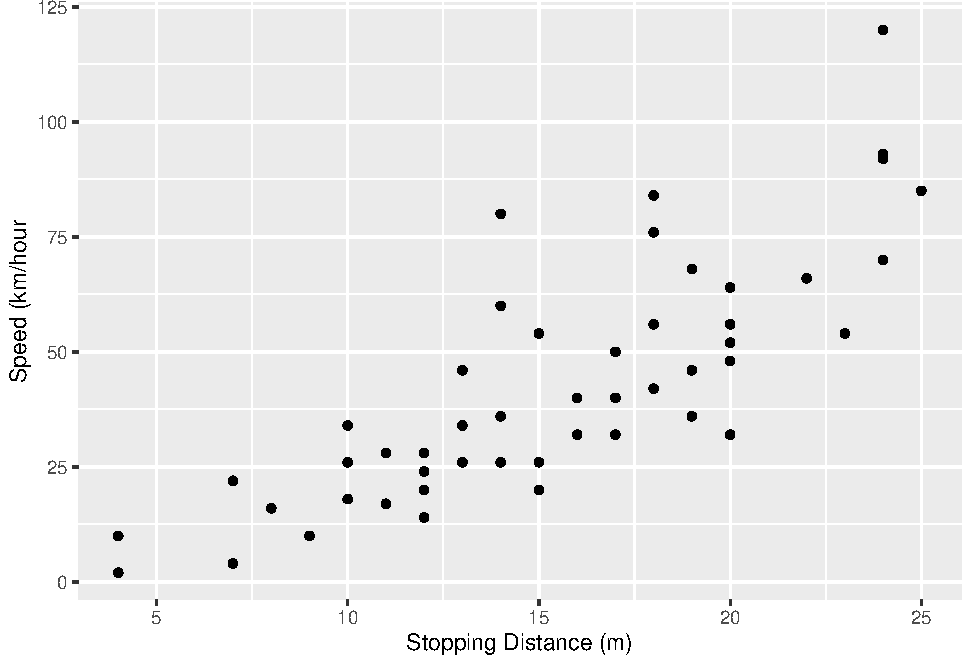
\includegraphics{Introduction-to-Experimental-Design-and-Analysis_files/figure-latex/unnamed-chunk-65-1.pdf}

There are a three things we should immediately notice in this figure. The first is that there is a positive relationship. The second is that it appears to be a bit non-linear, even \emph{exponential}. Third, it looks like there is more variation out at high speeds than at low speeds.

Let's ignore all of this for the moment and fit the model and acquire the diagnostics.

\begin{Shaded}
\begin{Highlighting}[]
\NormalTok{mod\_dist }\OtherTok{\textless{}{-}} \FunctionTok{lm}\NormalTok{(dist }\SpecialCharTok{\textasciitilde{}}\NormalTok{ speed, }\AttributeTok{data =}\NormalTok{ cars)}
\FunctionTok{autoplot}\NormalTok{(mod\_dist)}
\end{Highlighting}
\end{Shaded}

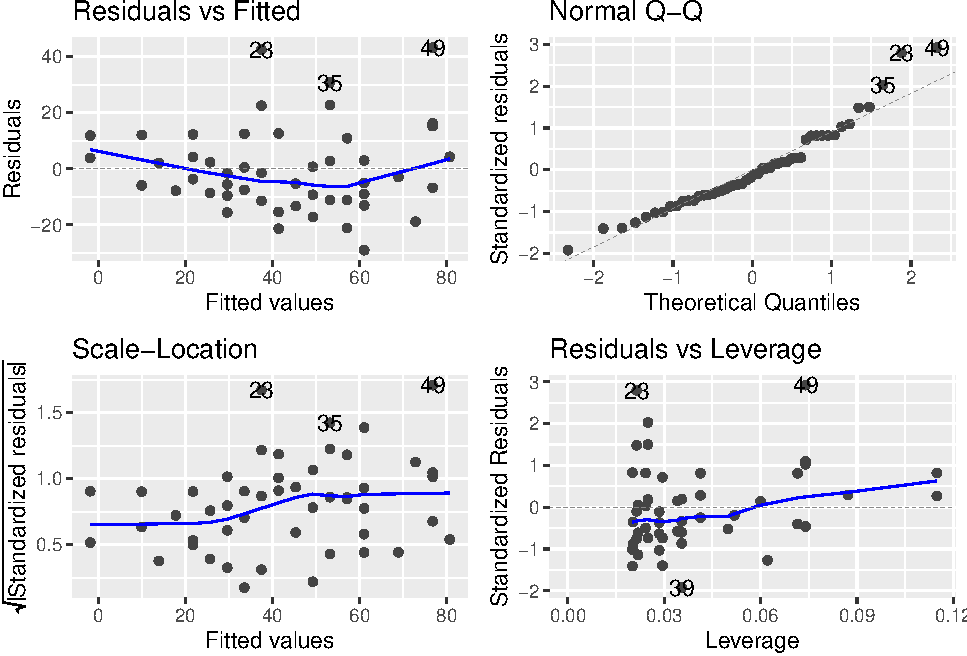
\includegraphics{Introduction-to-Experimental-Design-and-Analysis_files/figure-latex/unnamed-chunk-66-1.pdf}

OK - our preliminary assessment about non-linearity and non-constant variance appears to be spot on! There are systematic departures from the linear model indicated by the upper left plot.

Here we add a line to the data (plot) to understand why the residuals in the upper-left panel is u-shaped. Make sure you get the idea that the majority of the \textbf{data} are \emph{above} then \emph{below} then \emph{above} the line as you move across the graph. This generates residuals that have the pattern we see!

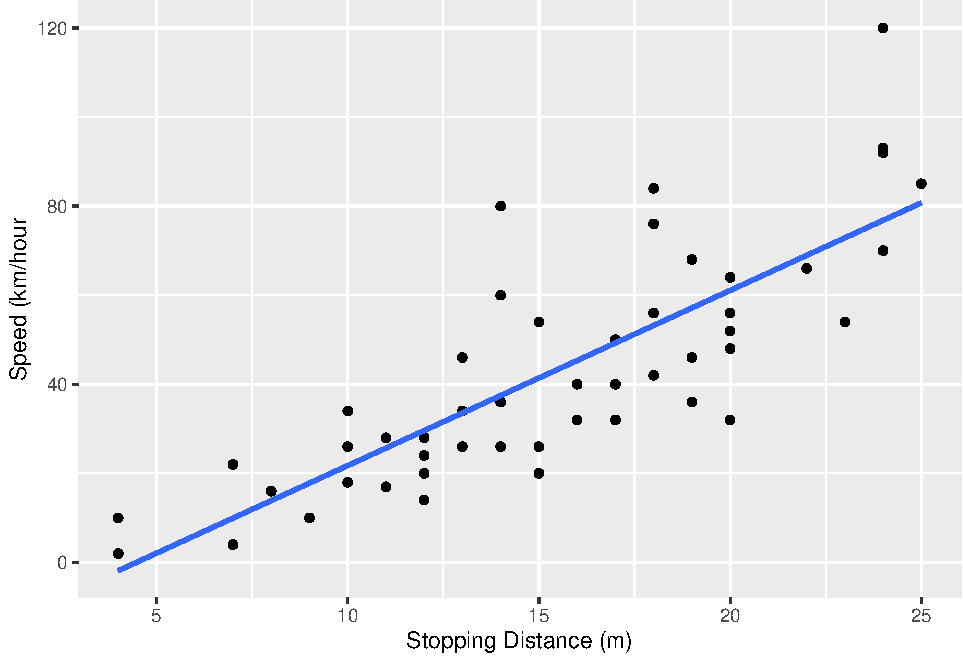
\includegraphics{Introduction-to-Experimental-Design-and-Analysis_files/figure-latex/unnamed-chunk-67-1.pdf}

The lower left panel of the residuals/diagnostics indicates that the variance does increase with the mean.

\hypertarget{interlude-1---inference-before-fixing-the-problem}{%
\subsection{Interlude 1 - Inference before fixing the problem}\label{interlude-1---inference-before-fixing-the-problem}}

I want to have us look at this model now before moving on. If we ignore the residuals, we end up with a strong conclusion that there is a positive linear relationship between stopping distance and speed.

\begin{Shaded}
\begin{Highlighting}[]
\FunctionTok{anova}\NormalTok{(mod\_dist)}
\end{Highlighting}
\end{Shaded}

\begin{verbatim}
## Analysis of Variance Table
## 
## Response: dist
##           Df Sum Sq Mean Sq F value   Pr(>F)    
## speed      1  21186 21185.5  89.567 1.49e-12 ***
## Residuals 48  11354   236.5                     
## ---
## Signif. codes:  0 '***' 0.001 '**' 0.01 '*' 0.05 '.' 0.1 ' ' 1
\end{verbatim}

\begin{Shaded}
\begin{Highlighting}[]
\FunctionTok{summary}\NormalTok{(mod\_dist)}
\end{Highlighting}
\end{Shaded}

\begin{verbatim}
## 
## Call:
## lm(formula = dist ~ speed, data = cars)
## 
## Residuals:
##     Min      1Q  Median      3Q     Max 
## -29.069  -9.525  -2.272   9.215  43.201 
## 
## Coefficients:
##             Estimate Std. Error t value Pr(>|t|)    
## (Intercept) -17.5791     6.7584  -2.601   0.0123 *  
## speed         3.9324     0.4155   9.464 1.49e-12 ***
## ---
## Signif. codes:  0 '***' 0.001 '**' 0.01 '*' 0.05 '.' 0.1 ' ' 1
## 
## Residual standard error: 15.38 on 48 degrees of freedom
## Multiple R-squared:  0.6511, Adjusted R-squared:  0.6438 
## F-statistic: 89.57 on 1 and 48 DF,  p-value: 1.49e-12
\end{verbatim}

\hypertarget{solving-the-problem-i-the-non-linearity}{%
\subsection{Solving the Problem I: The Non-linearity}\label{solving-the-problem-i-the-non-linearity}}

In order to fix this problem, we can take note from our first example in chapter 1 and fit a multiple regression model with a polynomial!

\begin{Shaded}
\begin{Highlighting}[]
\NormalTok{mod\_dist\_nonLin }\OtherTok{\textless{}{-}} \FunctionTok{lm}\NormalTok{(dist }\SpecialCharTok{\textasciitilde{}}\NormalTok{ speed }\SpecialCharTok{+} \FunctionTok{I}\NormalTok{(speed}\SpecialCharTok{\^{}}\DecValTok{2}\NormalTok{), }\AttributeTok{data =}\NormalTok{ cars)}
\FunctionTok{autoplot}\NormalTok{(mod\_dist\_nonLin)}
\end{Highlighting}
\end{Shaded}

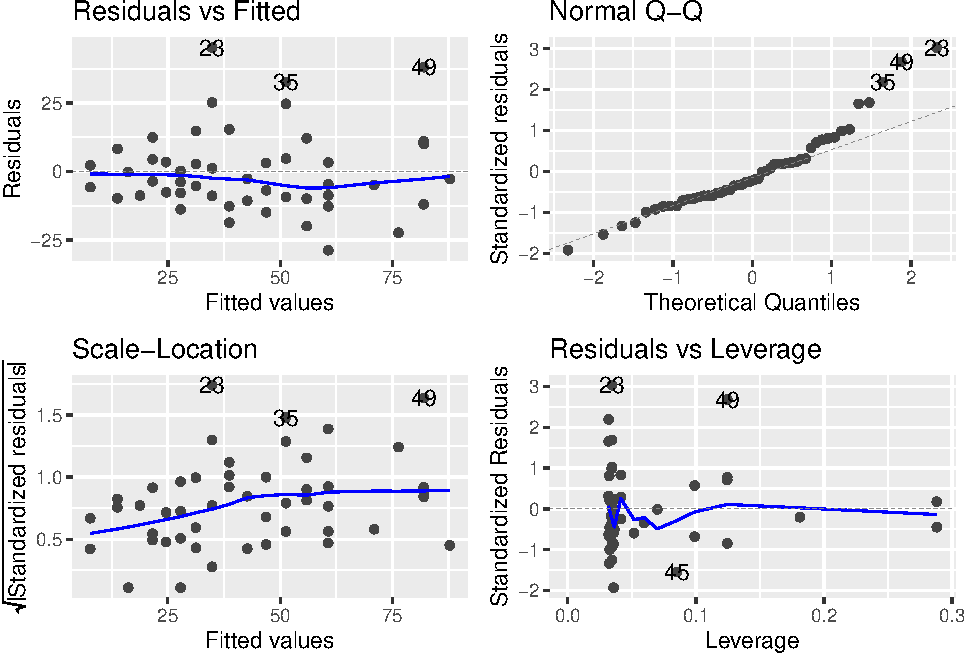
\includegraphics{Introduction-to-Experimental-Design-and-Analysis_files/figure-latex/unnamed-chunk-69-1.pdf}

Wow. That's a massive improvement on the diagnostic that indicated a systematic departure from the linear relationship between dist and speed. But\ldots. we still have non-constant variance - the variation in predicted distance is still increasing with the mean.

\hypertarget{interlude-2---inference-before-fixing-both-problems}{%
\subsection{Interlude 2 - Inference before fixing both problems}\label{interlude-2---inference-before-fixing-both-problems}}

As above, lets look at what the model tells us:

\begin{Shaded}
\begin{Highlighting}[]
\FunctionTok{anova}\NormalTok{(mod\_dist\_nonLin)}
\end{Highlighting}
\end{Shaded}

\begin{verbatim}
## Analysis of Variance Table
## 
## Response: dist
##            Df  Sum Sq Mean Sq F value    Pr(>F)    
## speed       1 21185.5 21185.5  91.986 1.211e-12 ***
## I(speed^2)  1   528.8   528.8   2.296    0.1364    
## Residuals  47 10824.7   230.3                      
## ---
## Signif. codes:  0 '***' 0.001 '**' 0.01 '*' 0.05 '.' 0.1 ' ' 1
\end{verbatim}

\begin{Shaded}
\begin{Highlighting}[]
\FunctionTok{summary}\NormalTok{(mod\_dist\_nonLin)}
\end{Highlighting}
\end{Shaded}

\begin{verbatim}
## 
## Call:
## lm(formula = dist ~ speed + I(speed^2), data = cars)
## 
## Residuals:
##     Min      1Q  Median      3Q     Max 
## -28.720  -9.184  -3.188   4.628  45.152 
## 
## Coefficients:
##             Estimate Std. Error t value Pr(>|t|)
## (Intercept)  2.47014   14.81716   0.167    0.868
## speed        0.91329    2.03422   0.449    0.656
## I(speed^2)   0.09996    0.06597   1.515    0.136
## 
## Residual standard error: 15.18 on 47 degrees of freedom
## Multiple R-squared:  0.6673, Adjusted R-squared:  0.6532 
## F-statistic: 47.14 on 2 and 47 DF,  p-value: 5.852e-12
\end{verbatim}

Hmm. That's interesting. We've added a term to the model to capture that hint of the non-linearity. There are two ways we might think this is `unjustified'. First, there is no evidence that this new term is significant. Second, we can formally compare the two models, giving us a p-value that's familiar from the tables above.

\begin{Shaded}
\begin{Highlighting}[]
\FunctionTok{anova}\NormalTok{(mod\_dist\_nonLin, mod\_dist)}
\end{Highlighting}
\end{Shaded}

\begin{verbatim}
## Analysis of Variance Table
## 
## Model 1: dist ~ speed + I(speed^2)
## Model 2: dist ~ speed
##   Res.Df   RSS Df Sum of Sq     F Pr(>F)
## 1     47 10825                          
## 2     48 11354 -1   -528.81 2.296 0.1364
\end{verbatim}

One might stop here and return to the data and the diagnostics and thing, hmmm\ldots{} that systematic departure issue? Not really a big deal after all\ldots. but lets carry on.

\hypertarget{solving-the-problem-ii-non-constant---increasing-variance}{%
\subsection{Solving the Problem II: Non-constant - increasing variance}\label{solving-the-problem-ii-non-constant---increasing-variance}}

One of the ways to `fix' this problem, is to make an assumption that the variance is proportional to the mean.

In the absence of this, the relationship is \(\sigma^{2} * speed\) - as speed increases, the variance increases. But if we assume that the variance is proportional, we get \(1/speed * \sigma^{2} * speed\)\ldots..

To do this in the model, we can use the \emph{weights} argument:

\begin{Shaded}
\begin{Highlighting}[]
\NormalTok{mod\_dist\_nonLin\_weight }\OtherTok{\textless{}{-}} \FunctionTok{lm}\NormalTok{(dist }\SpecialCharTok{\textasciitilde{}}\NormalTok{ speed }\SpecialCharTok{+}\FunctionTok{I}\NormalTok{(speed}\SpecialCharTok{\^{}}\DecValTok{2}\NormalTok{), }\AttributeTok{weights =} \DecValTok{1}\SpecialCharTok{/}\NormalTok{speed, }\AttributeTok{data =}\NormalTok{ cars)}
\FunctionTok{autoplot}\NormalTok{(mod\_dist\_nonLin\_weight)}
\end{Highlighting}
\end{Shaded}

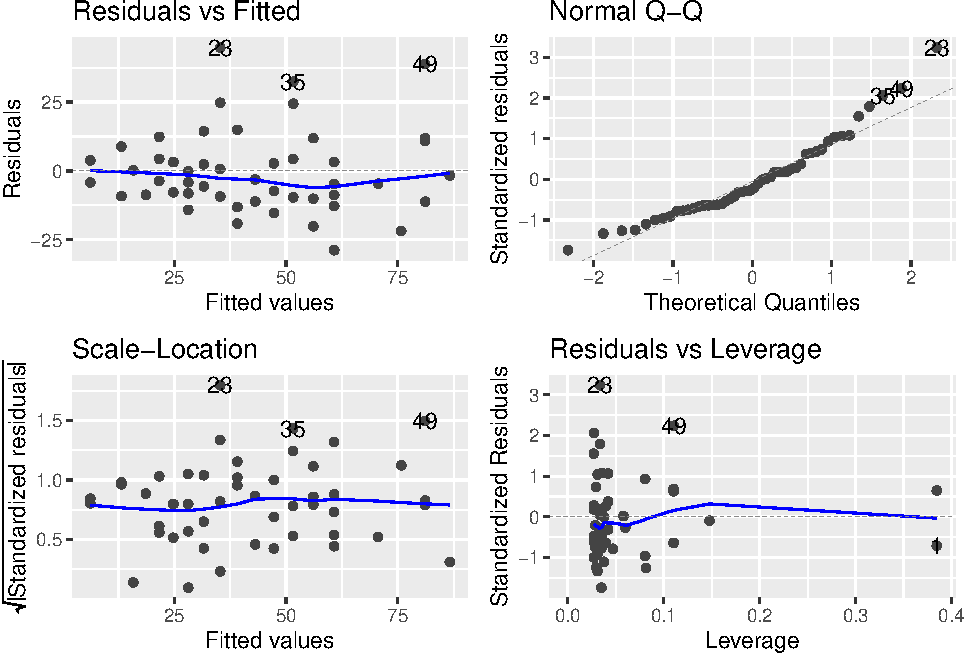
\includegraphics{Introduction-to-Experimental-Design-and-Analysis_files/figure-latex/unnamed-chunk-72-1.pdf}

Super. We now have a model where we capture the non-linearity using a polynomial and capture the issue of increasing variance by making the model reflect our assumption that different observations have different variances.

\hypertarget{interlude-3---inference-with-both-things-corrected.}{%
\subsection{Interlude 3 - Inference with both things corrected.}\label{interlude-3---inference-with-both-things-corrected.}}

OK. Now we are ready for using the anova table and summary table to make inference and update our figure.

\hypertarget{anova-tables-with-multiple-explantory-variables.}{%
\section{Anova Tables with multiple explantory variables.}\label{anova-tables-with-multiple-explantory-variables.}}

In previous exercises, we've used \texttt{anova()} to generate the anova table, F-statistics and p-values to test our hypotheses. It's very important to note that \texttt{anova()} makes a sequential sums of square calculation.

In our ANCOVA example, the model we fit was \texttt{lm(log(weight)\ \textasciitilde{}\ log(height)\ *\ sex,\ data\ =\ Davis)}. We know this expanded to \texttt{log(height)\ +\ sex\ +\ log(height):sex}.

When we reviewed the Anova Table, there were four rows corresponding to each of these three terms (2 main effects and 1 interaction) and the residual (remaining) variation.

In this table produced by \texttt{anova()}, we read it like this. First, we ask how much variation is explained by log(height). Having explained this variation, and left some unexplained, how much is then explained by sex. Finally, having explained some variation by log(height) and some of the remaining then by sex, can we explain any more by allowing slopes to vary (the interaction).

The key thing to note here is that this was a sequence. Sometimes this is fine - all we are interested in is the last line, for example, testing the hypothesis that the effect of height on weight varied by sex. This makes sense when we've designed an experiment to test a hypothesis.

However, in multiple regression, like our example with speed and distance, we need to worry about the order. It's really important too worry about this when we've NOT done a manipulative and designed experiment. This is because the terms in the model can be collinear. In an experiment, treatments are always independent. In observations studies, or when we start making polynomials, variables become non-independent.

Collinearity occurs when:

-One of the predictor variables is a function of another as in speed and speed\^{}2
-Your design is unbalanced, generating a non-orthogonal design -- note not all unbalanced designs are non-orthogonal.

How do we avoid using the sequence? Well, let's introduce the trick, and then reveal how it's working.

The trick is \texttt{Anova()} - not the big A. We call it \textbf{Big-A Anova}. It's in the \texttt{car} package.

\begin{Shaded}
\begin{Highlighting}[]
\FunctionTok{Anova}\NormalTok{(mod\_dist\_nonLin\_weight)}
\end{Highlighting}
\end{Shaded}

\begin{verbatim}
## Anova Table (Type II tests)
## 
## Response: dist
##            Sum Sq Df F value Pr(>F)
## speed       12.72  1  0.9009 0.3474
## I(speed^2)  34.44  1  2.4402 0.1250
## Residuals  663.42 47
\end{verbatim}

\hypertarget{explaining-the-trick}{%
\subsection{Explaining the Trick}\label{explaining-the-trick}}

So, this table is actually constructed by fitting two different models. One of those models is where \(speed\) is first and \(speed^{2}\) is second. The other model is where \(speed^{2}\) is first and \(speed\) is second.

\begin{Shaded}
\begin{Highlighting}[]
\FunctionTok{anova}\NormalTok{(}\FunctionTok{lm}\NormalTok{(dist }\SpecialCharTok{\textasciitilde{}}\NormalTok{ speed }\SpecialCharTok{+}\FunctionTok{I}\NormalTok{(speed}\SpecialCharTok{\^{}}\DecValTok{2}\NormalTok{), }\AttributeTok{weights =} \DecValTok{1}\SpecialCharTok{/}\NormalTok{speed, }\AttributeTok{data =}\NormalTok{ cars))}
\end{Highlighting}
\end{Shaded}

\begin{verbatim}
## Analysis of Variance Table
## 
## Response: dist
##            Df  Sum Sq Mean Sq  F value    Pr(>F)    
## speed       1 1609.18 1609.18 114.0024 3.704e-14 ***
## I(speed^2)  1   34.44   34.44   2.4402     0.125    
## Residuals  47  663.42   14.12                       
## ---
## Signif. codes:  0 '***' 0.001 '**' 0.01 '*' 0.05 '.' 0.1 ' ' 1
\end{verbatim}

\begin{Shaded}
\begin{Highlighting}[]
\FunctionTok{anova}\NormalTok{(}\FunctionTok{lm}\NormalTok{(dist }\SpecialCharTok{\textasciitilde{}} \FunctionTok{I}\NormalTok{(speed}\SpecialCharTok{\^{}}\DecValTok{2}\NormalTok{)}\SpecialCharTok{+}\NormalTok{speed, }\AttributeTok{weights =} \DecValTok{1}\SpecialCharTok{/}\NormalTok{speed, }\AttributeTok{data =}\NormalTok{ cars))}
\end{Highlighting}
\end{Shaded}

\begin{verbatim}
## Analysis of Variance Table
## 
## Response: dist
##            Df  Sum Sq Mean Sq  F value    Pr(>F)    
## I(speed^2)  1 1630.91 1630.91 115.5417 2.957e-14 ***
## speed       1   12.72   12.72   0.9009    0.3474    
## Residuals  47  663.42   14.12                       
## ---
## Signif. codes:  0 '***' 0.001 '**' 0.01 '*' 0.05 '.' 0.1 ' ' 1
\end{verbatim}

Pay close attention\ldots. can you see which of the \(speed\) and \(speed^{2}\) F and p-values from EACH of the two models are combined in the Big-A Anova table? It's from when the are \emph{last in the model}.

Technically, this is called a Type II anova table. Technically, it means that we are estimating the effects of each term, controlling for the other and respecting `marginality'. The Big-A Anova takes care of this \emph{`rotation of the position of the terms'} for us and produces the accurate test table we need.

For unbalanced data Type II ANOVA is recommended. In many cases the biology can be used to settle the question. Say for example if you're interested in the effect of a flower type on pollination after correcting for the effects of plant size - you know plant size affects the number of pollinator visits. Or if you have blocks (what are they?) then you might be interested in treatment affects after correcting for the effect of block.

\hypertarget{types-of-anova}{%
\section{Types of ANOVA}\label{types-of-anova}}

There are 3 types of ANOVA model based on how the sums of squares are divided. They hinge a bit on understanding \textbf{The Principle of Marginality }:

-A model with the A:B interaction must contain both the A and B main effects.
-The main effects are said to be marginal to the interaction.
-More generally if a higher-level interaction is included then all lower level interactions and main effects must be included.
-See Hector et al.~2010 Analysis of variance with unbalanced data: an update for ecology \& evolution. J Anim Ecol for a clear discussion of the different approaches.

The types of ANOVA:

Type I -- this is a sequential anova so order matters -- not very useful with unbalanced data or correlated predictors. Just fine for manipulative experiments and specific hypotheses captured by the `last term in the model'.

Type II -- measures effect of a predictor with all other predictors in the model, but obeys marginality principle. More sensible and conservative. A good standard.

Type III -- can test main effects after interactions, so test the main effect of A after the main effect of B and the A:B interaction ignores marginality principle.

This diagram may be valuable in helping you understand these ideas.

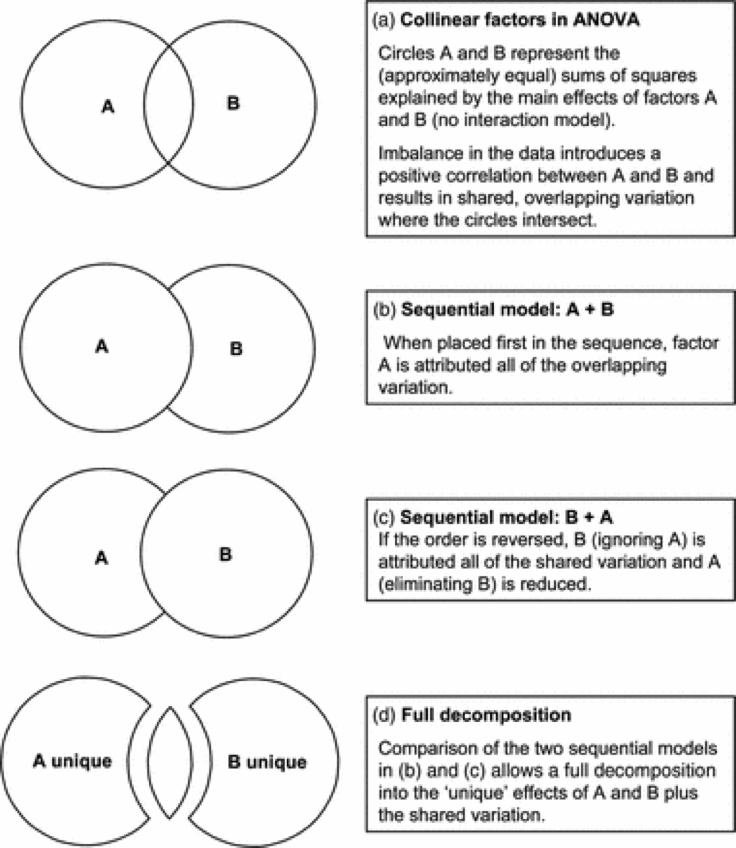
\includegraphics[width=10.22in]{images/VennModels}

\hypertarget{explaining-the-result---a-dose-of-reality}{%
\section{Explaining the result - a dose of reality}\label{explaining-the-result---a-dose-of-reality}}

So, hopefully that makes sense. We'll review more of that in the generalised linear model module with Dylan Childs.

What you might be wondering, however, is what the result means. We have no p-values that are \textless{} 0.05. Controlling for speed, there is no effect of speed\^{}2 and vice-versa. We kind of new that from our initial `sequential' assessment above\ldots.
OK. Whoa. This is weird, right?

Let's plot all of these three models we've made together with the data

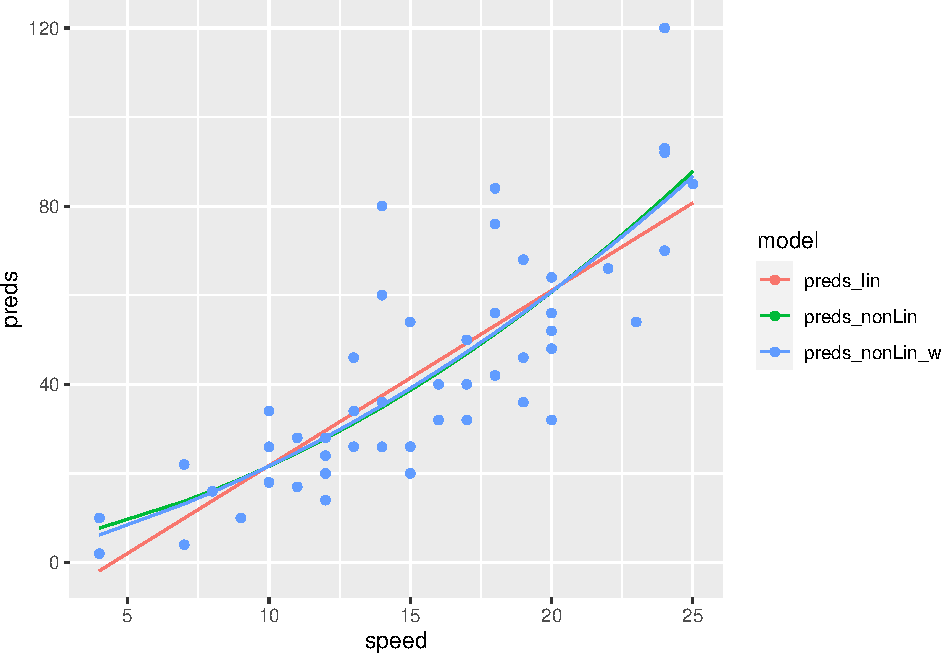
\includegraphics{Introduction-to-Experimental-Design-and-Analysis_files/figure-latex/unnamed-chunk-76-1.pdf}

At this point, we should ask, is the non-linear model makeing sense? We think it probably should, right? It's what the data look like and there was a hint of it in the residuals. But in the end, there is no evidence for a relationship.

Perhaps there is a better way to go about this. And in this better way a lesson in p-values and statistics.

\begin{quote}
Nothing beats a good question and an understanding of the mechanism you are actually evlauating.
\end{quote}

\hypertarget{a-mechanistic-model}{%
\section{A mechanistic model}\label{a-mechanistic-model}}

Here we have a mechanistic model stopping distance in made of:

\begin{itemize}
\tightlist
\item
  Thinking distance -- distance travelled while driver reacts so this is reaction time * speed
\item
  Braking distance -- which depends on the car's kinetic energy which is proportional to speed\^{}2
\end{itemize}

So we expect a model of the form -- note that there is NO intercept

\(Distance = \beta_{1}*Speed + \beta_{2}*speed^{2}\)

We can fit this model really simply with that trick of -1 \ldots. and all of a sudden\ldots.

\begin{Shaded}
\begin{Highlighting}[]
\CommentTok{\# fit model without intercept}
\NormalTok{mechMod }\OtherTok{\textless{}{-}} \FunctionTok{lm}\NormalTok{(dist }\SpecialCharTok{\textasciitilde{}}\NormalTok{ speed }\SpecialCharTok{+}\FunctionTok{I}\NormalTok{(speed}\SpecialCharTok{\^{}}\DecValTok{2}\NormalTok{) }\SpecialCharTok{{-}} \DecValTok{1}\NormalTok{, }\AttributeTok{weights =} \DecValTok{1}\SpecialCharTok{/}\NormalTok{speed, }\AttributeTok{data =}\NormalTok{ cars)}

\CommentTok{\# all the inferences}
\FunctionTok{anova}\NormalTok{(mechMod)}
\end{Highlighting}
\end{Shaded}

\begin{verbatim}
## Analysis of Variance Table
## 
## Response: dist
##            Df Sum Sq Mean Sq  F value    Pr(>F)    
## speed       1 5997.7  5997.7 433.8850 < 2.2e-16 ***
## I(speed^2)  1  137.1   137.1   9.9154  0.002818 ** 
## Residuals  48  663.5    13.8                       
## ---
## Signif. codes:  0 '***' 0.001 '**' 0.01 '*' 0.05 '.' 0.1 ' ' 1
\end{verbatim}

\begin{Shaded}
\begin{Highlighting}[]
\FunctionTok{Anova}\NormalTok{(mechMod)}
\end{Highlighting}
\end{Shaded}

\begin{verbatim}
## Anova Table (Type II tests)
## 
## Response: dist
##            Sum Sq Df F value   Pr(>F)   
## speed       92.60  1  6.6990 0.012727 * 
## I(speed^2) 137.06  1  9.9154 0.002818 **
## Residuals  663.51 48                    
## ---
## Signif. codes:  0 '***' 0.001 '**' 0.01 '*' 0.05 '.' 0.1 ' ' 1
\end{verbatim}

\begin{Shaded}
\begin{Highlighting}[]
\FunctionTok{summary}\NormalTok{(mechMod)}
\end{Highlighting}
\end{Shaded}

\begin{verbatim}
## 
## Call:
## lm(formula = dist ~ speed + I(speed^2) - 1, data = cars, weights = 1/speed)
## 
## Weighted Residuals:
##     Min      1Q  Median      3Q     Max 
## -6.4315 -2.3314 -0.8756  1.6428 11.9808 
## 
## Coefficients:
##            Estimate Std. Error t value Pr(>|t|)   
## speed       1.28525    0.49657   2.588  0.01273 * 
## I(speed^2)  0.08764    0.02783   3.149  0.00282 **
## ---
## Signif. codes:  0 '***' 0.001 '**' 0.01 '*' 0.05 '.' 0.1 ' ' 1
## 
## Residual standard error: 3.718 on 48 degrees of freedom
## Multiple R-squared:  0.9024, Adjusted R-squared:  0.8983 
## F-statistic: 221.9 on 2 and 48 DF,  p-value: < 2.2e-16
\end{verbatim}

\begin{Shaded}
\begin{Highlighting}[]
\CommentTok{\# plotting}
\NormalTok{plotMech }\OtherTok{\textless{}{-}}\NormalTok{ cars }\SpecialCharTok{\%\textgreater{}\%} 
  \FunctionTok{mutate}\NormalTok{(}\AttributeTok{preds =} \FunctionTok{predict}\NormalTok{(mechMod))}

\FunctionTok{ggplot}\NormalTok{(plotMech, }\FunctionTok{aes}\NormalTok{(}\AttributeTok{x =}\NormalTok{ speed, }\AttributeTok{y =}\NormalTok{ dist))}\SpecialCharTok{+}
  \FunctionTok{geom\_point}\NormalTok{()}\SpecialCharTok{+}
  \FunctionTok{geom\_line}\NormalTok{(}\FunctionTok{aes}\NormalTok{(}\AttributeTok{y =}\NormalTok{ preds))}
\end{Highlighting}
\end{Shaded}

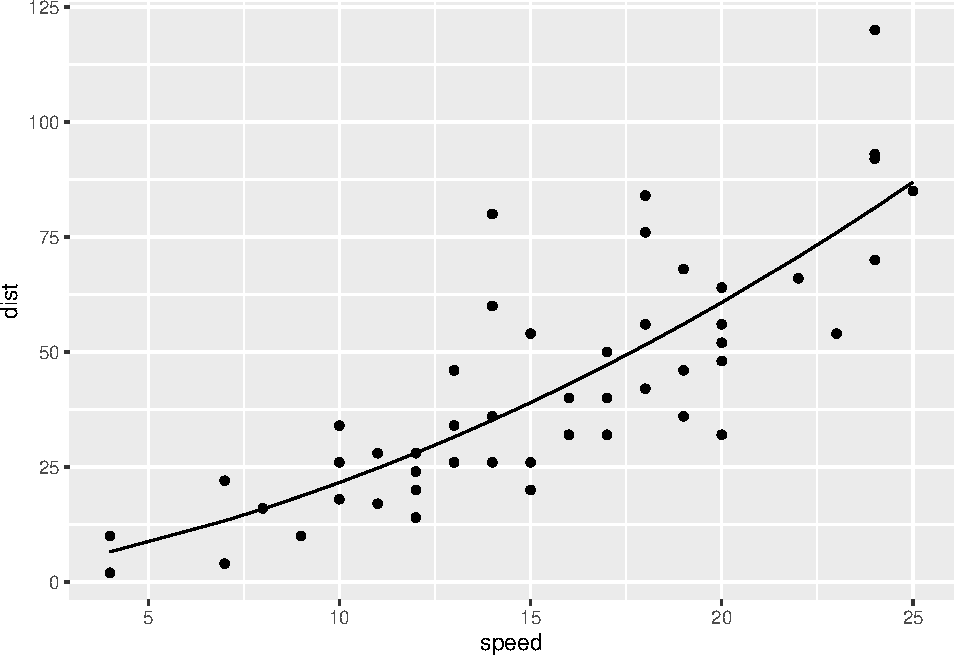
\includegraphics{Introduction-to-Experimental-Design-and-Analysis_files/figure-latex/unnamed-chunk-77-1.pdf}

\hypertarget{the-take-home-messages}{%
\section{The Take Home Messages}\label{the-take-home-messages}}

This example is not out of the ordinary of what you might face with your own data. The recipe for success in data analysis is a bit different from what you might expect.

\begin{enumerate}
\def\labelenumi{\arabic{enumi}.}
\tightlist
\item
  Design experiments to test hypotheses with Randomisation, Replication and Reducing Error in mind.
\item
  Think about your question and the mechanisms expected to give rise to the pattern
\item
  Plot your data and look at the patterns.
\item
  Fit appropriate models. Models for experiments are easier to define than models from survey and observation. Models for experiments don't have to worry as much about collinearity\ldots.
\item
  Don't follow the p-value.
\item
  Eat Biscuits
\end{enumerate}

\hypertarget{a-final-overview}{%
\chapter{A final Overview}\label{a-final-overview}}

  \bibliography{book.bib,packages.bib}

\end{document}
